% Created with jtex v.1.0.20
\documentclass[a4paper,11pt,oneside]{book}
\usepackage[top=2cm, bottom=2cm, left=2cm, right=2cm]{geometry}
\usepackage[T1]{fontenc}
\usepackage[utf8]{inputenc}
\usepackage{lmodern}
\usepackage{graphicx}
\usepackage{caption}
\usepackage{natbib}
\usepackage{xcolor}
\usepackage{changepage}
\usepackage{framed}
\usepackage{hyperref}
\usepackage{amssymb}
\usepackage{symbols}
\usepackage{cancel}

\bibliographystyle{abbrvnat}

% Make list items more compact
\usepackage{enumitem}
\setlist[itemize]{noitemsep, topsep=0pt}

%%%%%%%%%%%%%%%%%%%%%%%%%%%%%%%%%%%%%%%%%%%%%%%%%%
%%%%%%%%%%%%%%%%%%%%  imports  %%%%%%%%%%%%%%%%%%%
\usepackage{amsmath}
\usepackage{booktabs}
\usepackage{url}
%%%%%%%%%%%%%%%%%%%%%%%%%%%%%%%%%%%%%%%%%%%%%%%%%%


\hypersetup{
  colorlinks,
  linkcolor={black},
  citecolor={black},
  urlcolor={black}
}

% Style quotes
\definecolor{darkblue}{rgb}{0.0, 0.0, 0.55}
\definecolor{quoteshade}{rgb}{0.95, 0.95, 1}
\renewenvironment{quote}{%
  \def\FrameCommand{%
    \hspace{1pt}%
    {\color{darkblue}\vrule width 2pt}%
    {\color{quoteshade}\vrule width 4pt}%
    \colorbox{quoteshade}%
  }%
  \MakeFramed {\advance\hsize-\width \FrameRestore}%
  \noindent\hspace{-8pt}% disable indenting first paragraph
  \begin{adjustwidth}{0pt}{0pt}% adjust as needed
  \vspace{2pt}\vspace{2pt}%
}
{%
  \vspace{2pt}\end{adjustwidth}\endMakeFramed%
}

\title{\Huge \textbf{Skript FEM I + II}}
\author{\textsc{Prof. Dr.-Ing Steffen Beese}}

\begin{document}
\sloppy

\frontmatter
\maketitle

\tableofcontents
% \listoffigures
% \listoftables

\mainmatter

% \include{preface.tex}
% \include{acknowledgements.tex}

\chapter{Modul: Einführung in die FEM}

\section{Einführung}

\subsection{Numerische Simulation im Konstruktionsprozess}

\begin{figure}[!htbp]
\centering
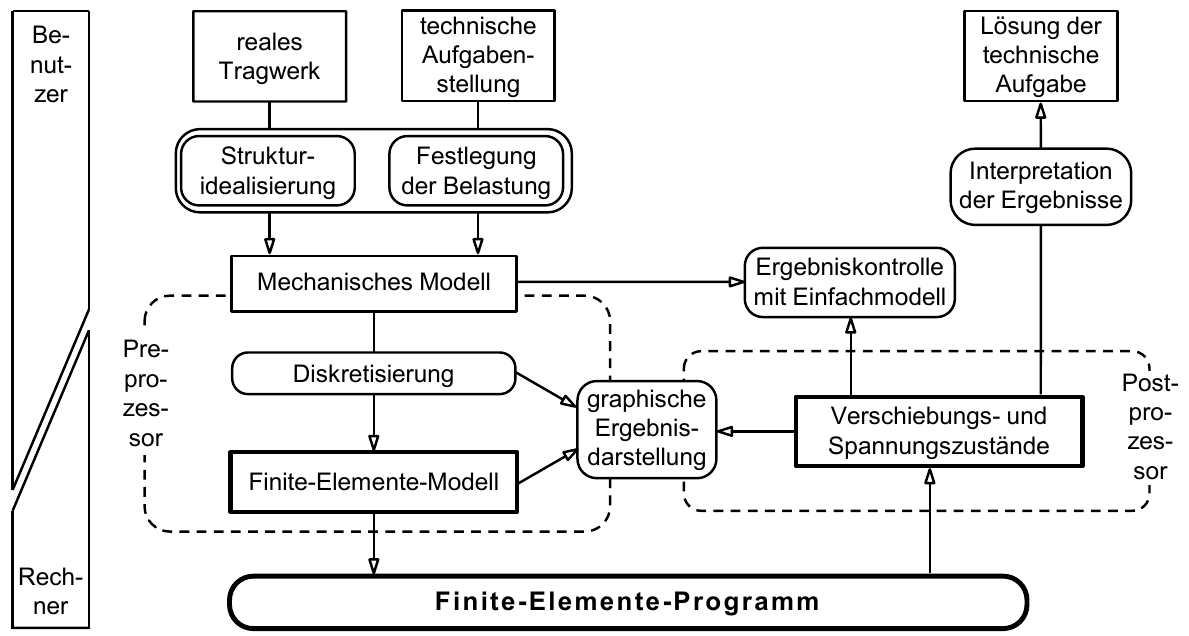
\includegraphics[width=0.7\linewidth]{files/Konstruktionsprozess-354f76ee1694c7cb48ad196b299f0eb9.png}
\caption[]{Einordnung numerischer Simulation in den Konstruktionsprozess nach \cite{knothe1991finite}}
\label{konstruktionsprozess}
\end{figure}

Finite-Elemente-Programme spielen eine wichtige Rolle bei der Untersuchung realer Tragwerke und technischer Aufgabenstellungen. Dieses leistungsfähige Tool ermöglicht es beispielsweise, die Integrität einer Pkw-Karosserie oder eines Rahmentragwerks zu analysieren, indem die Simulation eines Crash-Vorgangs durchgeführt wird oder die Traglast eines Bauteils berechnet wird. Für die virtuelle Produktentwicklung und eine prototypenfreie (oder prototypenarme) Entwicklung ist die Finite-Elemente-Methode aus den Entwicklungsabteilungen nicht mehr wegzudenken.

Der Weg zu einer validen FE-Simulation ist mehrstufig und interdisziplinär. In Abbildung Figure~\ref{konstruktionsprozess} sind die eigentlichen Schritte, die die Finite-Elemente-Methode betreffen, durch einen dicken Rahmen gekennzeichnet. Die vor- und nachgelagerte Prozesskette sollte von dem/der berechnenden Ingenieur/in eng begleitet werden, denn die Ergebnisse einer Simulation können nur so gut sein wie die Eingangsdaten: \textbf{Garbage in, garbage out}.

Zunächst wird die reale Struktur und ihre Belastung definiert und anschlie$\beta$end in geeigneter Weise abstrahiert:

\begin{itemize}
\item Genügt eine 2D-Berechnung oder gar eine 1D-Berechnung?
\item Welche geometrischen Details flie$\beta$en in die Simulation ein?
\item Kann ich die tatsächliche Last abstrahieren?
\item etc.
\end{itemize}

Das resultierende mechanische Modell ist somit eine idealisierte Darstellung der realen Problemstellung. Es geht darum, unwichtige Details wegzulassen, um die Berechnungen effizient und fokussiert zu halten, während gleichzeitig alle relevanten Belastungen präzise definiert werden müssen.

Auf die Modellierung folgt die Diskretisierung in finite Elemente. Dies sind kleine, standardisierte geometrische Objekte, auf denen die physikalischen Modellgleichungen gelöst werden. Mehr hierzu in späteren Kapiteln. Die Diskretisierung wird über sogenannte \textit{Preprozessoren} generiert. In modernen FE-Softwarepaketen sind diese Programmeinheiten integriert. Für gesonderte Diskretisierungsanforderungen gibt es jedoch auch Spezialsoftware wie:

\begin{itemize}
\item \href{https://altair.com/hypermesh/}{Hypermesh}
\item \href{https://www.beta-cae.com/}{Ansa}
\item \href{https://gmsh.info/}{Gmsh}
\end{itemize}

um nur einige zu nennen.
Zur Diskretisierung gehört nicht nur die Unterteilung des Gebietes in Finite Elemente. Auch die Belastungen müssen aus dem mechanischen Modell diskretisiert werden.

Das erstellte Finite-Elemente-Modell dient als Grundlage für die weiterführenden Berechnungen mit der gewählten FEM-Software - dem \textit{Prozessor}. Innerhalb des Programms wird aus den Eingabedaten ein, in der Regel nichtlineares, Gleichungssystem generiert und gelöst, das schlie$\beta$lich Aufschluss über relevante Grö$\beta$en wie Verschiebungen, Dehnungen, Spannungen, Wärmefluss und Temperaturverteilung gibt. Da die Menge an Ergebnisdaten bei gro$\beta$en Problemen erheblich sein kann, sind \textit{Postprozessoren} unverzichtbar, um eine übersichtliche und grafische Auswertung zu gewährleisten. Auch diese sind in kommerziellen FE-Systemen integriert, und auch hier haben sich für bestimmte Anwendungsfälle spezialisierte Softwarelösungen etabliert:

\begin{itemize}
\item \href{https://www.paraview.org/}{Paraview}
\item \href{https://tecplot.com/}{Tecplot}
\item \href{https://www.beta-cae.com/}{Ansa}
\item \href{https://www.gns-mbh.com/products/animator4/}{Animator4}
\end{itemize}

um auch hier nur einige zu nennen.

Der wichtigste Schritt für den/die Entwicklungsingenieur/in bei der FE-Simulation ist die anschlie$\beta$ende Auswertung und Bewertung der Ergebnisse. Man sollte den Resultaten stets mit einem gewissen Ma$\beta$ an Skepsis begegnen und entsprechende Kontrollen hinsichtlich Plausibilität und Grö$\beta$enordnung durchführen. Dies kann durch Vergleiche mit Einfachmodellen und experimentellen Untersuchungen unterstützt werden.

Letztlich muss der/die Anwender/in die Resultate im Kontext der technischen Aufgabe interpretieren. Sollten die Ergebnisse nicht zufriedenstellend sein, kann es notwendig sein, die Rechnung zu wiederholen. Dies kann Änderungen im Finite-Elemente-Modell, der Idealisierung der Struktur oder der Festlegung der Belastungen nach sich ziehen. Nur durch diese iterative Vorgehensweise lässt sich ein genaues und verlässliches Bild des untersuchten technischen Systems gewinnen.

%  -+-+-+-+-+-+-AI-SPLIT

%  - **Nutzung von Finite-Elemente-Programmen**
%   - Anwendung zur Untersuchung realer Tragwerke unter technischen Aufgabenstellungen
%   - Beispiele für reale Strukturen: Pkw-Karosserie, Stockwerkrahmen
%   - Beispiele für technische Aufgaben: Simulation eines Crash-Vorgangs, Ermittlung der Traglast
% 
% - **Erstellung des mechanischen Modells**
%   - Idealisierte Darstellung der Struktur entscheidend
%   - Weglassen von unwichtigen Strukturdetails
%   - Festlegung der relevanten Belastungen
% 
% - **Diskretisierung in finite Elemente**
%   - Manuelle Diskretisierung möglich bei kleinen Strukturen
%   - Rechnerunterstützung erforderlich bei komplexen Strukturen wie Fahrzeugkarosserien oder Flugzeugen
%   - Nutzung von Preprozessoren zur Modellerzeugung und grafischen Kontrolle
% 
% - **Finite-Elemente-Modell als Basis für Berechnungen**
%   - Bereitstellung von Eingabedaten für FEM-Programme
%   - Internes Generieren und Lösen von Gleichungssystemen
%   - Bestimmung relevanter Größen wie Verschiebungen und Schnittkräfte
%   - Verwendung von Postprozessoren zur übersichtlichen Darstellung der Ergebnisse
% 
% - **Kritische Bewertung der FEM-Ergebnisse**
%   - Notwendigkeit des Misstrauens gegenüber FEM-Ergebnissen
%   - Durchführung von Kontrollen für Plausibilität und Größenordnung der Ergebnisse
%   - Vergleich mit Einfachmodellen und experimentellen Untersuchungen
% 
% - **Interpretation und Anpassung**
%   - Interpretation der Ergebnisse im Kontext der technischen Aufgabe
%   - Mögliche Wiederholung der Rechnung bei nicht zufriedenstellenden Ergebnissen
%   - Anpassung des Finite-Elemente-Modells, Idealisierung der Struktur oder Belastungsfestlegung ggf. notwendig

\subsubsection{Der Systembegriff}

\begin{quote}
Ein System besteht aus einer Menge von Elementen (Teilsystemen), die Eigenschaften besitzen und durch Beziehungen miteinander verknüpft sind. Das System wird durch eine Systemgrenze von der Umgebung abgegrenzt und steht mit der Umgebung durch Ein- und Ausgangsgrö$\beta$en in Beziehung. Die Funktion eines Systems kann durch den Unterschied der dem Zweck entsprechenden Ein- und Ausgangsgrö$\beta$en beschrieben werden. Die Systemelemente können selbst wiederum Systeme sein, die aus Elementen und Beziehungen bestehen. \cite{ehrlenspiel2013integrierte}
\end{quote}

Die Definition eines Systems umfasst mehrere wesentliche Schritte:

\begin{enumerate}
\item \textbf{Identifikation der Systemgrenzen}: Hier wird festgelegt, was zum System gehört und was nicht. Diese Abgrenzung ist entscheidend, um den Fokus der Analyse zu bestimmen und irrelevante Einflüsse auszuschlie$\beta$en.


\item \textbf{Bestimmung der Systemelemente}: In diesem Schritt werden die Komponenten identifiziert, die Teil des Systems sind. Diese Komponenten können physikalische Objekte, biologische Organismen, soziale Gruppen, technische Bauteile etc. sein.


\item \textbf{Beschreibung der Beziehungen zwischen den Systemelementen}: Hier wird untersucht, wie die einzelnen Komponenten miteinander interagieren.
\end{enumerate}

Ein gut definiertes System ist entscheidend für die Genauigkeit und Zuverlässigkeit der Simulationsergebnisse. Nur wenn alle relevanten Komponenten und deren Interaktionen korrekt erfasst und modelliert werden, können valide Aussagen über das Systemverhalten getroffen werden.

\textbf{Zustand, Zustandsgrö$\beta$e, Zustandsvariable}

In der numerischen Simulation wird der Zustand eines Systems durch eine Reihe von Zustandsgrö$\beta$en oder Zustandsvariablen beschrieben. Diese Variablen repräsentieren die Eigenschaften des Systems zu einem bestimmten Zeitpunkt.

\begin{itemize}
\item \textbf{Zustand}: Der Zustand eines Systems ist eine vollständige Beschreibung des Systems zu einem bestimmten Zeitpunkt. Er umfasst alle relevanten Informationen, die notwendig sind, um das Verhalten des Systems zu verstehen und vorherzusagen. Der Zustand ist somit eine Momentaufnahme des Systems, die alle wesentlichen Eigenschaften und Charakteristika beinhaltet.


\item \textbf{Zustandsgrö$\beta$e / Zustandsvariable}: Eine Zustandsgrö$\beta$e ist eine messbare Eigenschaft des Systems, die den Zustand des Systems beschreibt. Beispiele für Zustandsgrö$\beta$en sind Temperatur, Druck, Spannung und Verformung. Diese Grö$\beta$en sind oft physikalische Messwerte, die direkt beobachtet oder gemessen werden können. Es handelt sich bei Zustandsvariablen zudem meist um Felder, das hei$\beta$t, sie haben eine räumliche und zeitliche Abhängigkeit.


\item \textbf{Systemverhalten}: Das Systemverhalten beschreibt, wie sich das System im Laufe der Zeit entwickelt. Es umfasst die Dynamik und die Reaktionen des Systems auf äu$\beta$ere Einflüsse und interne Prozesse. Das Systemverhalten ist somit die zeitliche Entwicklung des Zustands des Systems und kann durch die zeitliche Abfolge von Punkten im Zustandsraum beschrieben werden.
\end{itemize}

%  -+-+-+-+-+-+-AI-SPLIT

\subsubsection{Klassifikation von Systemen}

Systeme können nach verschiedenen Ordnungskriterien klassifiziert werden. In der nachfolgenden Tabelle sind die wichtigsten Kriterien und deren Beschreibung aufgeführt.

\bigskip\noindent
\begin{tabular}{p{\dimexpr 0.500\linewidth-2\tabcolsep}p{\dimexpr 0.500\linewidth-2\tabcolsep}}
\toprule
\textbf{Klassifikation} & \textbf{Beschreibung} \\
\hline
\textbf{Statisch} & Systeme, deren Verhalten unabhängig von der Zeit ist; Zustände ändern sich nicht. \\
\textbf{Quasistatisch} & Systeme, die sich langsam ändern, sodass sie zu jedem Zeitpunkt als statisch betrachtet werden können. \\
\textbf{Dynamisch} & Systeme, deren Verhalten sich mit der Zeit ändert; Zustände entwickeln sich über die Zeit. \\
\textbf{Zeitkontinuierlich} & Systeme, die zu jedem Zeitpunkt einen definierten Zustand haben; Änderungen erfolgen kontinuierlich. \\
\textbf{Zeitdiskret} & Systeme, die nur zu bestimmten Zeitpunkten Zustandsänderungen aufweisen; Änderungen erfolgen in diskreten Schritten. \\
\textbf{Ereignisorientiert} & Systeme, deren Verhalten durch bestimmte Ereignisse ausgelöst wird; Änderungen treten in Reaktion auf Ereignisse auf. \\
\textbf{Deterministisch} & Systeme, deren Verhalten vollständig durch Anfangsbedingungen und Regeln bestimmt ist; keine Zufälligkeit. \\
\textbf{Stochastisch} & Systeme, deren Verhalten durch Zufallsprozesse beeinflusst wird; es gibt eine gewisse Unsicherheit im Verhalten. \\
\bottomrule
\end{tabular}

\bigskip\begin{figure}[!htbp]
\centering
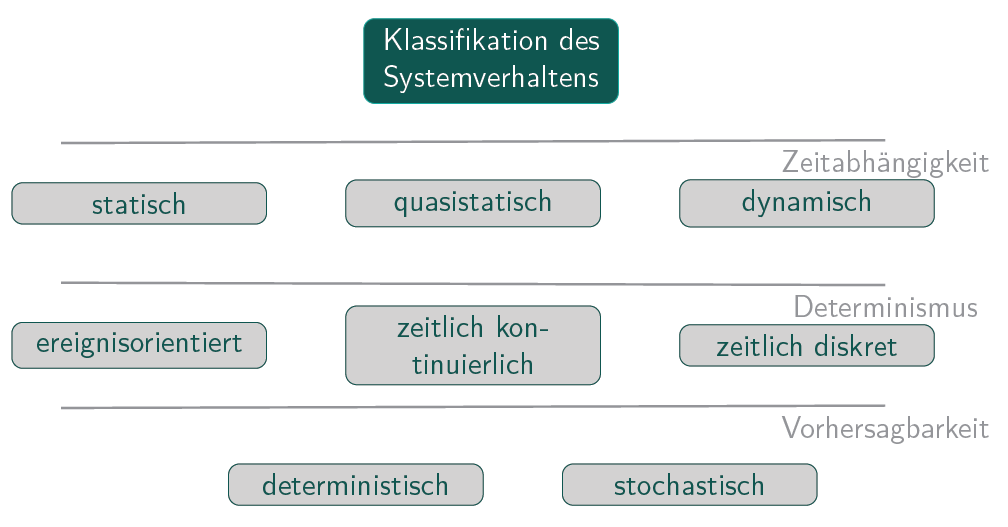
\includegraphics[width=0.7\linewidth]{files/Systemverhalten-eb19fad1d9ad10e9c65047ac7b46ad78.png}
\caption[]{Klassifikation von Systemen nach ihrem Verhalten}
\label{systemverhalten}
\end{figure}

\subsubsection{Der Modellbegriff}

In der Entwicklung mechatronischer Systeme spielen die VDI-Richtlinien 2206 und 2211 eine zentrale Rolle. Diese Richtlinien bieten eine methodische Grundlage für die Modellbildung, die ein physikalisch-mathematisches Abbild eines technischen Bauelements, einer Baugruppe oder eines komplexen Systems darstellt.

\textbf{Modellbildung und ihre Bedeutung}

Modelle sind materielle oder immaterielle Gebilde, die geschaffen werden, um für einen bestimmten Zweck ein Original zu repräsentieren. Sie können als Abbildungen oder Nachbildungen von Originalen betrachtet werden. Die Modellbildung beinhaltet die Darstellung eines physikalisch-mathematischen Modells eines vorhandenen Systems oder eines zu entwickelnden Systems. Der Zweck der Modellbildung besteht darin, das Original durch das Modell zu ersetzen und es als Stellvertreter des Originals zu nutzen, um Rückschlüsse auf das Original zu ziehen.

Modelle können somit als zweckgerichtete, vereinfachte Abbildungen oder Nachbildungen von Originalen aufgefasst werden. Sie umfassen eine Vielzahl von Konstrukten, darunter Anschauungsmodelle, Prototypen, Konstruktionszeichnungen, Schaltpläne, mathematische Gleichungen, aber auch Gedankenmodelle bzw. mentale Modelle, Vorstellungen und Bilder.

\textbf{Anforderungen an Modelle}

Modelle müssen original- und realitätsnah sein, um charakteristische Eigenschaften und Verhalten des Originals genau zu beschreiben. Der Modellzweck hängt von den Lebensphasen des Produkts ab, und es ist wichtig, ein angemessenes Aufwand-/Nutzen-Verhältnis zu gewährleisten. Der Aufwand für Modellierung und Analyse ist eng mit dem Detaillierungsgrad (Granularität) des Modells verbunden. Eine sehr genaue Modellierung ist nicht immer notwendig; Unsicherheiten können den Nutzen eines detaillierten Modells in Frage stellen.

Das Modellverhalten muss im Gültigkeitsbereich dem realen Systemverhalten entsprechen, um die Modellgültigkeit zu gewährleisten. Das Verhalten resultiert aus den Eigenschaften der Modellelemente und deren Verknüpfungen. Bei mehreren geeigneten Modellierungsansätzen sollte die einfachste Methode bevorzugt werden, um die Modelleffizienz zu maximieren. Es gibt keine allgemeinen Regeln für die Herleitung eines einfachen, effizienten und gültigen Modells; vielmehr sind Erfahrung und Vorwissen entscheidend.

%  -+-+-+-+-+-+-AI-SPLIT

\subsubsection{Modellbildung}

\begin{framed}
\textbf{Ziel der Modellbildung}\\
Modellbildung ist die Schaffung eines Modells, das dem Untersuchungszweck entspricht und demgemä$\beta$ verändert und ausgewertet werden kann, um damit Rückschlüsse auf das Original ziehen zu können.
\end{framed}

\begin{figure}[!htbp]
\centering
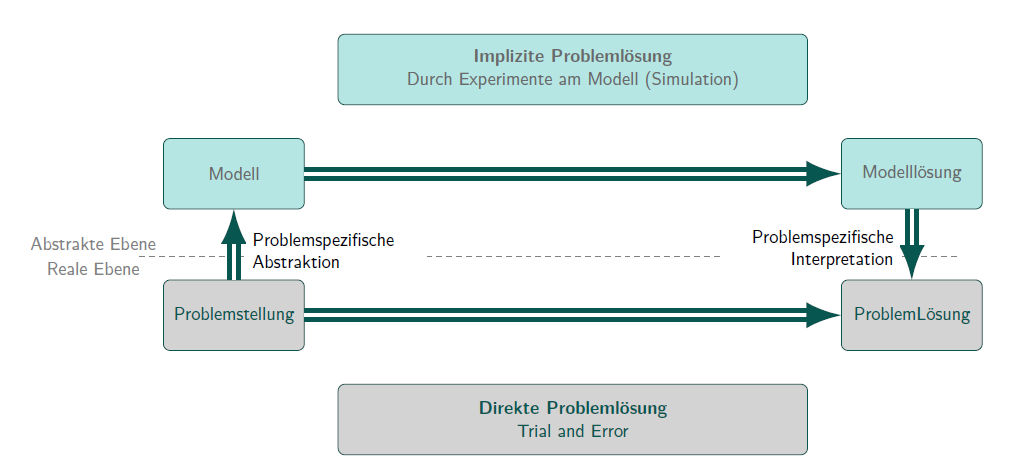
\includegraphics[width=0.7\linewidth]{files/Problemloesung-e104c317db14666b2fd6f513a8ca1a48.png}
\caption[]{Problemlösung im Ingenieurwesen nach \cite{vajna2009cax}}
\label{problemlösung}
\end{figure}

Die Modellabstraktion ist ein zentraler Bestandteil der Ingenieurwissenschaft, da sie die Realität einer Berechnung zugänglich macht. Durch die Abstraktion werden irrelevante Details vernachlässigt, während die relevanten Details erhalten bleiben. Das Ziel ist es, ein Modellergebnis zu erzielen, das eine hohe Relevanz für die Lösung der realen Problemstellung aufweist.

\textbf{Modellabstraktion als Grundlage für Analyse und Design}

Ein Modell dient als Grundlage für die Analyse und das Design von Systemen. Durch die Konzentration auf die spezifischsten und wichtigsten Merkmale und die Abstraktion von unwichtigen Eigenschaften und Details wird die Komplexität der Problemstellung reduziert. Diese Vereinfachung ist bereits ein Ziel der Analyse, da sie die Handhabbarkeit der Problemstellung ermöglicht. Ohne eine solche Vereinfachung wären viele Problemstellungen innerhalb der praktischen Beschränkungen von Zeit und Ressourcen äu$\beta$erst komplex zu simulieren oder nicht effektiv zu analysieren.

\textbf{Vorteile einfacher Modelle}

Einfachere Modelle sind von Natur aus leichter zu entwickeln, zu verstehen und zu modifizieren. Dies ist besonders wertvoll in iterativen Designprozessen, in denen häufige Aktualisierungen von Modellen erforderlich sind. Abstrakte Modelle können als gemeinsame Sprache für Ingenieure aus verschiedenen Disziplinen oder mit unterschiedlichem Fachwissen dienen. Sie reduzieren Missverständnisse und ermöglichen eine effektivere Zusammenarbeit in Ingenieurprojekten.

Darüber hinaus erfordern einfachere Modelle weniger Rechenleistung und Zeit für die Lösung. Dies ermöglicht mehr Iterationen, Sensitivitätsanalysen und die Untersuchung von Designalternativen innerhalb angemessener Zeitrahmen. Die Vereinfachung durch Modellabstraktion trägt somit wesentlich zur Effizienz und Effektivität des gesamten Design- und Analyseprozesses bei.

\begin{figure}[!htbp]
\centering
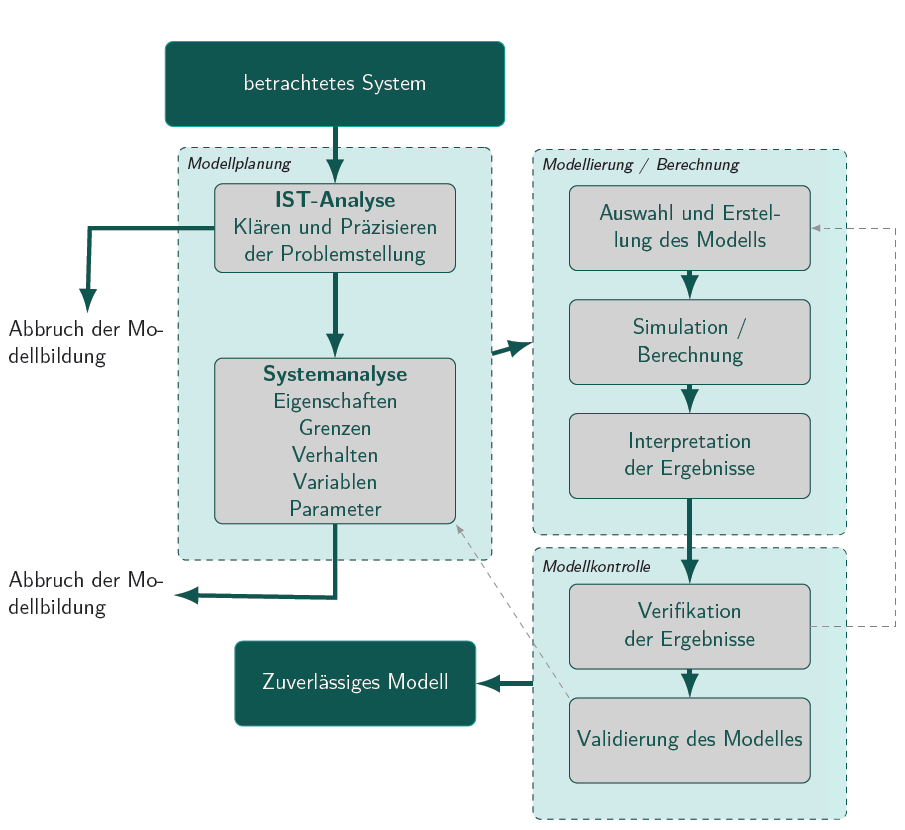
\includegraphics[width=0.7\linewidth]{files/Modellbildung-df30eb7519c2d11046de71abe95091b6.png}
\caption[]{Modellbildungsprozess nach \cite{vajna2009cax}}
\label{modellbildung}
\end{figure}

In Abbildung Modellbildung ist der Modellbildungsprozess dargestellt. Die Modellplanung beginnt mit einer IST-Analyse, in der die Aufgabenstellung zu klären und zu präzisieren ist. Dabei treten typischerweise Fragen auf wie (\cite{vajna2009cax}):

\begin{itemize}
\item Was ist das zu untersuchende Original (System, Elemente, Systemgrenzen)?
\item Welche Fragestellungen sollen behandelt werden (Festlegung des Modellzwecks)?
\item Welche Sichtweisen auf das zu untersuchende Original (Systemaspekte, Bewertungskriterien) sind für den Modellzweck notwendig?
\item Welche Eigenschaften müssen für die gewünschte Bewertung (z.~B. zur Eigenschaftsabsicherung) herangezogen werden?
\item Welche Effekte (Details) müssen daher berücksichtigt oder können vernachlässigt werden?
\item Welche Testsituationen sind zu untersuchen („Lastfälle``, Testszenarien, „Use Cases``)?
\item Welche Parameter bzw. Zustandsgrö$\beta$en eines mathematischen Modells werden als vorgegeben (Parameter), welche als Zustandsvariablen betrachtet?
\item Welche Ergebnisse sind zur Klärung der Fragestellungen erforderlich und in welcher Form sollen die Ergebnisdaten aufbereitet und dokumentiert werden (Ergebnisdarstellung und Dokumentation)?
\item Welche Relevanz und Signifikanz haben die zu erwartenden Ergebnisse in Bezug auf die Fragestellungen? Wird die Fragestellung durch die Ergebnisse auch wirklich beantwortet?
\end{itemize}

%  -+-+-+-+-+-+-AI-SPLIT

\textbf{Verifikation und Validierung}

Jedes Modell stellt lediglich eine mehr oder weniger genaue Annäherung an das Original (z.B. ein reales System) dar. Daher ist es nach der Modellentwicklung notwendig, zu überprüfen, ob das Modell mit seinen Idealisierungen das zu untersuchende Original ausreichend genau abbildet. Die Verifikation untersucht, ob sich das Modell grundsätzlich plausibel verhält, und bezieht sich dabei auf das Modellverhalten, unabhängig von Vergleichen mit einem konkreten Original. Die Modellverifikation betrifft somit die Überprüfung der Plausibilität des Modellverhaltens an sich, also für „fiktive`` Originale. Die Validierung hingegen liefert eine Aussage darüber, ob das erstellte Modell konkrete Originale hinreichend beschreibt und in welchem Bereich das Modell gültig ist (Grenzen des Modells).

\subsubsection{Ansätze zur Abstraktion mechanischer Modelle}

Zur Abstraktion mechanischer Modelle können folgende Ansätze angewendet werden:

\begin{enumerate}
\item Vereinfachung der Geometrie

\begin{itemize}
\item Abstraktion durch einfachere geometrische Grundkörper
\item Komplexe Maschinenrahmen als Skelettstruktur aus Balken oder ein dünnwandiges Druckgefä$\beta$ als Schale modelliert werden
\end{itemize}


\item Dimensionsreduktion

\begin{itemize}
\item Übergang von einer 3D-Darstellung zu einer 2D-Darstellung (ebener Spannungszustand, ebener Dehnungszustand, rotationssymmetrisch) oder sogar 1D-Darstellung (Balken, Stäbe)
\end{itemize}


\item Vereinfachung der Materialeigenschaften

\begin{itemize}
\item Wenn angemessen, linear-elastische Materialmodelle anstelle komplexerer nichtlinearer oder anisotroper Modelle
\end{itemize}


\item Abstraktion der Randbedingungen

\begin{itemize}
\item Darstellung komplexer Lagerungen oder Lasten durch idealisierte Randbedingungen
\item Z. B. feste, gelenkige oder rollende Lagerungen oder durch die Verwendung von Punktlasten oder verteilten Lasten
\end{itemize}


\item Systemebenenabstraktion

\begin{itemize}
\item Subsysteme oder Komponenten werden als Black Boxes mit definierten Ein- und Ausgängen modelliert
\item Schwerpunkt auf ihrem Gesamtverhalten und nicht auf komplizierten internen Details
\item Ansatz besonders nützlich für die Analyse gro$\beta$er, komplexer Systeme, indem diese in kleinere, besser handhabbare Teile zerlegt werden
\end{itemize}


\item Vereinfachte physikalische Bilanzgleichung
\end{enumerate}

%  -+-+-+-+-+-+-AI-SPLIT

\begin{framed}
\textbf{Fragen zum Kapitel}\\
\textbf{Allgemeine Verständnisfragen zur numerischen Simulation}

\begin{itemize}
\item Was sind mögliche Zielstellungen der numerischen Simulation im Konstruktionsprozess?
\item Erläutern Sie den Begriff ``Garbage in, garbage out'' im Kontext von Finite-Elemente-Simulationen.
\item Beschreiben Sie die Schritte, die vor einer FE-Simulation durchgeführt werden müssen.
\item Nennen Sie zwei Kriterien für die Wahl zwischen einer 1D-, 2D- oder 3D-Finite-Elemente-Berechnung.
\end{itemize}

\textbf{Zum Thema Systembegriff}

\begin{itemize}
\item Wie wird ein System definiert und welche Elemente umfasst es?
\item Was sind die wesentlichen Schritte bei der Definition eines Systems?
\item Was versteht man unter Zustand und Zustandsgrö$\beta$e in der numerischen Simulation?
\end{itemize}

\textbf{Zur Klassifikation von Systemen}

\begin{itemize}
\item Nennen Sie drei Kriterien zur Klassifikation von Systemverhalten und beschreiben Sie diese.
\item Warum ist das Wissen über das Systemverhalten wichtig für die Simulation?
\end{itemize}

\textbf{Über den Modellbegriff}

\begin{itemize}
\item Welche Anforderungen sollten Modelle erfüllen?
\item Erklären Sie den Begriff ``Modellabstraktion'' und dessen Bedeutung im Ingenieurwesen.
\item Welche Vorteile bieten einfachere Modelle gegenüber komplexeren Modellen während des Design- und Analyseprozesses?
\end{itemize}

\textbf{Zum Modellbildungsprozess}

\begin{itemize}
\item Nennen Sie die wesentlichen Schritte im Modellbildungsprozess.
\item Welche Bedeutung haben Verifikation und Validierung in der Modellbildung?
\end{itemize}

\textbf{Ansätze zur Abstraktion mechanischer Modelle}

\begin{itemize}
\item Nennen Sie drei Ansätze zur Abstraktion mechanischer Modelle und erklären Sie diese kurz.
\item Was versteht man unter Dimensionsreduktion und wann wird sie angewendet?
\item In welchen Situationen ist eine Vereinfachung der Materialeigenschaften angebracht?
\end{itemize}

\textbf{Vertiefende Fragen zur Reflexion}

\begin{itemize}
\item Was ist der Unterschied zwischen der Verifikation und der Validierung eines Modells?
\item Was sind die Konsequenzen einer unzureichenden Modellvalidierung?
\item Wie kann eine kritische Bewertung der Ergebnisse einer FE-Simulation erfolgen?
\end{itemize}
\end{framed}

\input{FEMI_Skript-einf-hrung-modellklassifikation}

\subsubsection{Numerische Lösungsverfahren}

Der kontinuierliche Modellansatz führt zu Feldgleichungen in Form von partiellen Differentialgleichungen. Anwendungsgebiete sind hier die Strukturmechanik, der Stoff- und Wärmetransport sowie die Elektrostatik und viele weitere Bereiche. Diese partiellen Differentialgleichungen können in der Regel nicht analytisch gelöst werden, weshalb sich numerische Berechnungsschemata hierfür etabliert haben. Die heute gebräuchlichsten werden im Folgenden kurz beschrieben:

\begin{itemize}
\item Netzbasierte Methoden:\begin{itemize}
\item Finite-Elemente-Methode \textbf{(FEM)}
\item Finite-Volumen-Methode \textbf{(FVM)}
\item Finite-Differenzen-Methode \textbf{(FDM)}
\item Randelementmethode \textbf{(BEM)}
\item Discontinuous Galerkin Methods \textbf{(DG)}
\end{itemize}


\item Netzunabhängige Methoden:\begin{itemize}
\item Optimal Transport Method \textbf{(OTM)}
\item Element-Free Galerkin \textbf{(EFG)}
\item Moving Least Squares \textbf{(MLS)}
\end{itemize}


\item Kombination:\begin{itemize}
\item Material Point Method \textbf{(MPM)}
\end{itemize}


\item ...
\end{itemize}

Alle diese Methoden haben eine Gemeinsamkeit: Sie führen auf ein Gleichungssystem der Form:
\begin{equation}
\label{LGS}
\boldsymbol{Ax}=\boldsymbol{b}
\end{equation}
mit der Systemmatrix $\boldsymbol{A}$. Im Folgenden soll nur kurz auf die 4 am weitesten verbreiteten Methoden eingegangen werden.

%  -+-+-+-+-+-+-AI-SPLIT

\paragraph{Finite Differenzen Methode (FDM)}

Die Finite Differenzen Methode (FDM) ist ein numerisches Verfahren zur Lösung partieller Differentialgleichungen (PDEs), das auf der Approximation der Ableitungen durch Differenzenquotienten basiert. Hier sind die grundlegenden Schritte und Konzepte der FDM:

\begin{enumerate}
\item \textbf{Diskretisierung des Raums}: Der kontinuierliche Raum wird in ein Gitter unterteilt. Die Punkte auf diesem Gitter werden als Gitterpunkte bezeichnet.
\item \textbf{Approximation der Ableitungen}: Die Ableitungen in der PDE werden durch finite Differenzen approximiert. Zum Beispiel kann die erste Ableitung einer Funktion $u$ an einem Punkt $i$ durch den zentralen Differenzenquotienten approximiert werden:
\end{enumerate}
\begin{equation}
\frac{du}{dx} \approx \frac{u_{i+1} - u_{i-1}}{2\Delta x}
\end{equation}
oder durch den vorwärts gerichteten Differenzenquotienten:
\begin{equation}
\frac{du}{dx} \approx \frac{u_{i+1} - u_i}{\Delta x}
\end{equation}
\begin{enumerate}[resume]
\item \textbf{Aufstellen eines Gleichungssystems}: Durch das Einsetzen der approximierten Ableitungen in die ursprüngliche PDE wird ein System von algebraischen Gleichungen aufgestellt, das die Werte der Funktion an den Gitterpunkten beschreibt.
\item \textbf{Lösen des Gleichungssystems}: Das resultierende Gleichungssystem kann mit verschiedenen numerischen Verfahren gelöst werden.
\end{enumerate}

Die Finite Differenzen Methode ist einfach zu implementieren und eignet sich gut für Probleme mit regelmä$\beta$igen Gitterstrukturen. Sie hat jedoch Einschränkungen bei der Behandlung komplexer Geometrien und kann in der Nähe von Randbedingungen oder Singularitäten weniger genau sein.

%  -+-+-+-+-+-+-AI-SPLIT

\paragraph{Finite Volumen Methode (FVM)}

Die Finite Volumen Methode  ist ein numerisches Verfahren zur Lösung partieller Differentialgleichungen (PDEs), das insbesondere in der Strömungsmechanik und bei der Simulation von Transportphänomenen weit verbreitet ist. Hier sind die grundlegenden Schritte und Konzepte der FVM:

\begin{enumerate}
\item \textbf{Diskretisierung des Raums}: Der kontinuierliche Raum wird in eine endliche Anzahl von Kontrollvolumen unterteilt. Jedes Kontrollvolumen ist ein kleines Volumen, das um einen Gitterpunkt zentriert ist. Diese Volumina können regelmä$\beta$ig oder unregelmä$\beta$ig sein, je nach der Geometrie des Problems.
\item \textbf{Integralform der PDE und Flussdiskretisierung}: Die PDE wird in ihrer Integralform formuliert und über jedes Kontrollvolumen integriert. Durch Anwendung des Gauss'schen Integralsatzes wird die Integralform in eine Form umgewandelt, die die Flüsse an den Grenzen der Kontrollvolumen berücksichtigt. Die Flüsse an den Grenzen werden approximiert, häufig durch Mittelwerte der Variablen an den benachbarten Kontrollvolumen oder durch spezielle Interpolationsmethoden.
\item \textbf{Aufstellen eines Gleichungssystems}: Durch die Diskretisierung der Flüsse und das Einsetzen in die Integralform wird ein System von algebraischen Gleichungen aufgestellt, das die Werte der gesuchten Variablen an den Gitterpunkten beschreibt.
\item \textbf{Lösen des Gleichungssystems}: Das resultierende Gleichungssystem kann mit verschiedenen numerischen Verfahren gelöst werden.
\end{enumerate}

Die Finite Volumen Methode ist besonders vorteilhaft, da sie die Erhaltungsgesetze direkt in die Berechnungen integriert und somit eine physikalisch konsistente Lösung gewährleistet. Sie eignet sich gut für Probleme mit komplexen Geometrien und ist robust gegenüber nichtlinearen Effekten. FVM wird häufig in der Strömungsmechanik, Wärmeübertragung und anderen Bereichen eingesetzt, in denen der Transport von Stoffen oder Energie eine Rolle spielt.

%  -+-+-+-+-+-+-AI-SPLIT

\paragraph{Randelemente Methode (BEM)}

Die Randelemente Methode (BEM) ist ein numerisches Verfahren zur Lösung partieller Differentialgleichungen (PDEs), das sich auf die Randbedingungen des Problems konzentriert. Hier sind die grundlegenden Schritte und Konzepte der BEM:

\begin{enumerate}
\item \textbf{Reduktion des Problems auf den Rand}: Anstatt das gesamte Volumen des Problems zu diskretisieren, wird nur der Rand des betrachteten Gebiets in Betracht gezogen. Dies reduziert die Dimension des Problems, da nur die Randflächen (2D) oder Randlinien (1D) diskretisiert werden müssen.
\item \textbf{Formulierung der Integralgleichungen}: Die PDE wird in eine Integralform umgewandelt, die die Randbedingungen berücksichtigt. Diese Integralgleichungen beschreiben die Beziehung zwischen den Werten der gesuchten Funktion und ihren Ableitungen auf dem Rand des Gebiets.
\item \textbf{Diskretisierung des Randes}: Der Rand wird in eine endliche Anzahl von Elementen unterteilt, und die gesuchte Funktion wird durch Basisfunktionen approximiert, die auf diesen Elementen definiert sind. Dies führt zu einem System von algebraischen Gleichungen, das die Werte der gesuchten Funktion an den Randpunkten beschreibt.
\item \textbf{Lösen des Gleichungssystems}: Das resultierende Gleichungssystem kann mit verschiedenen numerischen Verfahren gelöst werden.
\end{enumerate}

Die Randelemente Methode ist besonders vorteilhaft, da sie die Dimension des Problems reduziert und somit die Anzahl der benötigten Berechnungen verringert. Sie ist besonders effektiv für Probleme mit unendlichen oder halbunendlichen Domänen, wie z.B. in der Elastizitätstheorie oder der Akustik. BEM ist jedoch oft auf Probleme mit linearen PDEs und gut definierten Randbedingungen beschränkt. Das hei$\beta$t, materielle Nichtlinearitäten können nicht berücksichtigt werden (keine Plastizität!).

%  -+-+-+-+-+-+-AI-SPLIT

\paragraph{Finite Elemente Methode (FEM)}

Die Finite-Elemente-Methode (FEM) ist ein weit verbreitetes numerisches Verfahren zur Lösung partieller Differentialgleichungen (PDEs), das insbesondere in der Ingenieurwissenschaft und der Physik Anwendung findet. Hier sind die grundlegenden Schritte und Konzepte der FEM:

\begin{enumerate}
\item \textbf{Diskretisierung des Gebiets}: Der kontinuierliche Raum wird in eine endliche Anzahl von kleinen, nicht überlappenden Elementen unterteilt, die zusammen ein Netz (Mesh) bilden. Diese Elemente können verschiedene Formen haben, wie Dreiecke, Vierecke (in 2D) oder Tetraeder, Hexaeder (in 3D).
\item \textbf{Aufstellen der Elementgleichungen}: Für jedes Element wird eine lokale Formulierung der PDE aufgestellt, die die physikalischen Gesetze und Randbedingungen berücksichtigt. Dies geschieht häufig durch die Anwendung des Prinzips der virtuellen Verrückungen oder der Galerkin-Methode, um die Differentialgleichung in eine schwache Form zu überführen.
\item \textbf{Zusammenfügen der Elementgleichungen}: Die lokalen Gleichungen der einzelnen Elemente werden zu einem globalen Gleichungssystem zusammengefügt. Dies geschieht unter Berücksichtigung der Koppelung zwischen benachbarten Elementen und der gemeinsamen Knotenpunkte.
\item \textbf{Lösen des Gleichungssystems}: Das resultierende globale Gleichungssystem wird mit numerischen Verfahren gelöst.
\end{enumerate}

Die Finite-Elemente-Methode ist besonders vorteilhaft, da sie komplexe Geometrien und Materialverhalten effizient behandeln kann. Sie ermöglicht die Analyse von statischen und dynamischen Problemen in verschiedenen Bereichen, wie Strukturmechanik, Wärmeübertragung und Fluiddynamik. FEM ist flexibel und anpassungsfähig, erfordert jedoch eine sorgfältige Netzgenerierung und kann bei sehr feinen Netzen rechenintensiv sein.

%  -+-+-+-+-+-+-AI-SPLIT

\paragraph{Zusammenfassung}

\begin{figure}[!htbp]
\centering
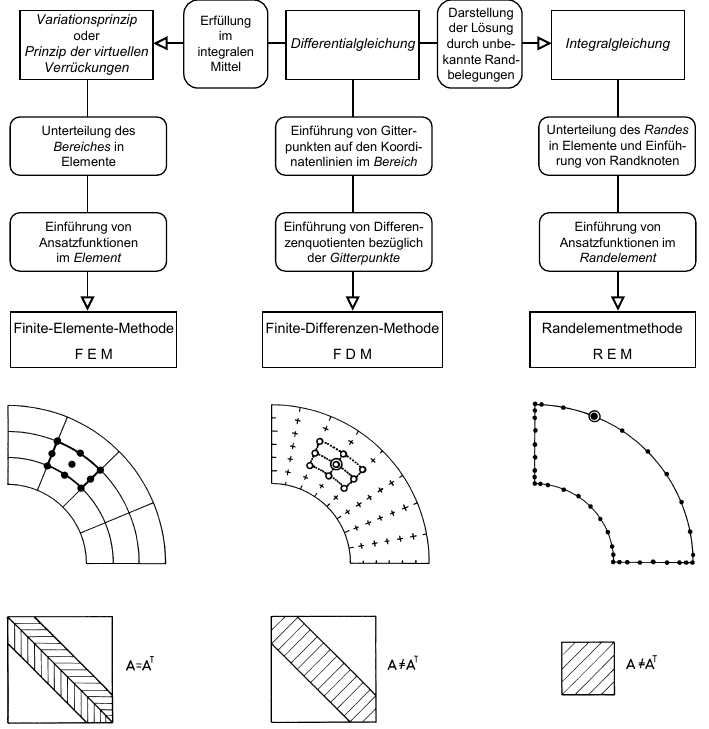
\includegraphics[width=0.7\linewidth]{files/Diskretisierungsverf-3291ac8fb462ef44b4d348533f5b41ac.png}
\caption[]{Vergleich verschiedener Diskretisierungsverfahren nach \cite{knothe1991finite}}
\label{diskretisierungsvergleich}
\end{figure}

Jede der oben genannten Methoden hat ihre Daseinsberechtigung für gewählte Problemstellungen. Für die Strukturmechanik hat sich die Finite-Elemente-Methode durchgesetzt, da sie am flexibelsten und effizientesten eingesetzt werden kann. Dies wird in Abbildung Figure~\ref{diskretisierungsvergleich} deutlich. Die resultierende Systemmatrix $A$ ist für viele Problemstellungen symmetrisch und weist eine ausgesprochene Bandstruktur auf, was für die Lösung des Gleichungssystems erhebliche Vorteile bringt.

\bigskip\noindent
\begin{tabular}{p{\dimexpr 0.200\linewidth-2\tabcolsep}p{\dimexpr 0.200\linewidth-2\tabcolsep}p{\dimexpr 0.200\linewidth-2\tabcolsep}p{\dimexpr 0.200\linewidth-2\tabcolsep}p{\dimexpr 0.200\linewidth-2\tabcolsep}}
\toprule
Methode & Dimension & Ansatz & Vorteile & Nachteile \\
\hline
\textbf{FEM} & Volumen & Diskretisierung des gesamten Gebiets in Elemente & Flexibel für komplexe Geometrien und Materialverhalten; gut für statische und dynamische Probleme & Erfordert sorgfältige Netzgenerierung; rechenintensiv bei feinen Netzen \\
\textbf{BEM} & Rand & Reduktion des Problems auf den Rand des Gebiets & Reduziert die Dimension des Problems; effizient bei unendlichen oder halbunendlichen Domänen & Beschränkt auf Probleme mit gut definierten Randbedingungen; oft nur für lineare PDEs geeignet \\
\textbf{FDM} & Volumen & Diskretisierung des Gebiets in Gitterpunkte & Einfach zu implementieren; gut für regelmä$\beta$ige Geometrien & Schwierigkeiten bei komplexen Geometrien; weniger genau in der Nähe von Singularitäten \\
\textbf{FVM} & Volumen & Diskretisierung des Gebiets in Kontrollvolumen & Berücksichtigt Erhaltungsgesetze direkt; robust bei nichtlinearen Effekten & Kann komplexer in der Implementierung sein; erfordert sorgfältige Flussapproximation \\
\bottomrule
\end{tabular}

\bigskip Jede Methode hat ihre eigenen Stärken und Schwächen, und die Wahl der Methode hängt oft von der spezifischen Anwendung ab.

%  -+-+-+-+-+-+-AI-SPLIT

\begin{framed}
\textbf{Fragen zum Kapitel}\\
\textbf{Numerische Lösungsverfahren}

\begin{itemize}
\item Nennen Sie drei Verfahren zur Lösung von partiellen Differentialgleichungen (Feldgleichungen).
\item Warum benötigen wir numerische Verfahren zur Lösung der Feldgleichungen?
\item In allen numerischen Verfahren werden die Feldgleichungen umgeformt. Was muss letztendlich bei allen Verfahren gelöst werden?
\item Welches numerische Verfahren ist besonders gut für Strömungsprobleme geeignet?
\item Nennen Sie drei Gründe, warum sich die FEM in der Strukturmechanik durchgesetzt hat?
\end{itemize}
\end{framed}

%  $
% \newcommand{\MtdFull}[1]{\frac{D \, #1}{D \, t}}
% \newcommand{\Pd}[2]{\frac{\partial #1}{\partial #2}}
% \newcommand{\dt}[1]{#1 ^{\bullet}}
% \newcommand{\dV}{\; \text{d}V}
% \newcommand{\dA}{\; \text{d}A}
% \newcommand{\dx}{\; \text{ d}x}
% \newcommand{\dy}{\; \text{ d}y}
% \newcommand{\dz}{\; \text{ d}z}
% \newcommand{\dxi}{\; \text{ d}\xi}
% \newcommand{\deta}{\; \text{ d}\eta}
% \newcommand{\dzeta}{\; \text{ d}\zeta}
% \newcommand{\grad}[1]{\text{grad}\left(#1\right)}
% \renewcommand{\div}[1]{\text{div} \left(#1\right)}
% \newcommand{\td}[1]{\dot{#1}}
% \newcommand{\tdd}[1]{\ddot{#1}}
% \newcommand{\T}{\rp{T}}
% \newcommand{\rp}[1]{^{\text{#1}}}
% \newcommand{\rs}[1]{_{\text{#1}}}
% \renewcommand{\bm}[1]{\boldsymbol{#1}}
% \newcommand{\e}{\epsilon}
% \newcommand{\eb}{\bm{\e}}
% \newcommand{\s}{\sigma}
% \newcommand{\sb}{\bm{\sigma}}
% $

%  ```{admonition} Todo
% :class: warning
% - [x] Motivation
% - [x] Lernziele
% - [x] Bilanzgleichungen
%    - [x] lokale Form 
%    - [x] Randbedingungen
%    - [x] Anwendung
%    - [x] Zusammenfassende Tabelle
% - [x] Kinematik
%    - [x] lineare Kinematik
% - [x] Materialmodellierung
%    - [x] Wärmeleitung nach Fourier
%    - [x] Lineare Elastizität
%    - [x] Ausblick
%    - [x] Ebener Spannungszustand
%    - [x] Ebener Verzerrungszustand
%    - [x] Rotationssymmetrie
% ```

%  -+-+-+-+-+-+-AI-SPLIT

\begin{framed}
\textbf{Lernziele}\\
\begin{itemize}
\item Wie werden mechanische Problemstellungen formuliert?
\item Was sind die Unbekannten der Bilanzgleichungen?
\item Welche Zutaten braucht man, um ein lösbares Problem zu erhalten?
\item Wie lauten die wesentlichen Bilanzgleichungen der Kontinuumsmechanik?
\item In welche Kategorien werden Randbedingungen untergliedert?
\item Wozu brauchen wir Materialmodelle?
\item Welche sind die grundlegenden Materialmodelle der Wärmeleitung, des Fluidtransports und der Strukturmechanik?
\item Mit welchen Vereinfachungen kann die Dimensionalität der Problemstellung reduziert werden?
\item Was sind die Voraussetzungen hierfür?
\end{itemize}
\end{framed}

\subsubsection{Mathematische Modellbildung in der Kontinuumstheorie}

In diesem Kapitel werden die grundlegenden Gleichungen der Kontinuumsmechanik vorgestellt. Dies dient als Ausgangspunkt für die numerische Lösung mechanischer Problemstellungen. Während der Vorstellung der Ausgangsgleichungen wird zudem die verwendete Notation eingeführt.

\paragraph{Notation}

Im Rahmen dieses Moduls wird die folgende symbolische Schreibweise verwendet:

\bigskip\noindent
\begin{tabular}{p{\dimexpr 0.333\linewidth-2\tabcolsep}p{\dimexpr 0.333\linewidth-2\tabcolsep}p{\dimexpr 0.333\linewidth-2\tabcolsep}}
\toprule
Tensorstufe & Symbol & Tensorschreibweise \\
\hline
Tensor der Stufe 0 (Skalar) & $a$, $b$, $\varphi$ & $a$, $b$, $\varphi$ \\
Tensor der Stufe 1 (Vektor) & $\bm{a}$, $\bm{b}$ & $a_i\bm{e}_i$, $b_i\bm{e}_i$ \\
Tensor der Stufe 2 (Dyade) & $\bm{A}$, $\bm{\sigma}$ & $A_{ij}\bm{e}_i\bm{e}_j$, $B_{ij}\bm{e}_i\bm{e}_j$ \\
Tensor der Stufe 4 & $\mathbb{C}$, $\mathbb{A}$ & $\mathbb{C}\bm{e}_i\bm{e}_j\bm{e}_k\bm{e}_l$, $\mathbb{A}\bm{e}_i\bm{e}_j\bm{e}_k\bm{e}_l$ \\
\bottomrule
\end{tabular}

Soweit möglich erhalten Tensoren der Stufe 2 Gro$\beta$buchstaben als Symbol, während Vektoren mit Kleinbuchstaben dargestellt werden. Handschriftlich wird ein Tensor durch einen Unterstrich repräsentiert $\underline{A}=\bm{A}$. Für Vektoren ist alternativ auch der Vektorpfeil gebräuchlich $\underline{a} = \vec{a} = \bm{a}$.

%  -+-+-+-+-+-+-AI-SPLIT

\paragraph{Bilanzgleichungen der Kontinuumsmechanik}

In diesem Abschnitt werden wir die grundlegenden Bilanzgleichungen der Kontinuumsmechanik einführen. Diese Gleichungen sind das Fundament für die Beschreibung des physikalischen Verhaltens und bilden den Ausgangspunkt für die Finite-Elemente-Methode. Die Bilanzgleichungen repräsentieren Erhaltungsprinzipien, die für jedes Kontinuum gelten, unabhängig von den spezifischen Materialeigenschaften. Die Bilanzgleichungen dienen als Bestimmungsgleichung für die Feldgrö$\beta$en:

\begin{itemize}
\item Druck $p(\bm{x},t)$
\item Verschiebung $\bm{u}(\bm{x},t)$
\item Temperatur $\theta(\bm{x},t)$.
\end{itemize}

Als Feldgrö$\beta$e bezeichnet man physikalische Grö$\beta$en, denen zu jedem Zeitpunkt $t$ und zu jedem materiellen Punkt $\bm{x}$ ein Wert zugeordnet wird.

Die vier wesentlichen Bilanzgleichungen sind:

\begin{itemize}
\item Massenerhaltung
\item Impulserhaltung
\item Drehimpulserhaltung (hieraus resultiert die Symmetrie des Spannungstensors $\bm{\sigma}$)
\item Energieerhaltung (1. Hauptsatz der Thermodynamik)
\end{itemize}

\subparagraph{Massenerhaltung}

\begin{figure}[!htbp]
\centering
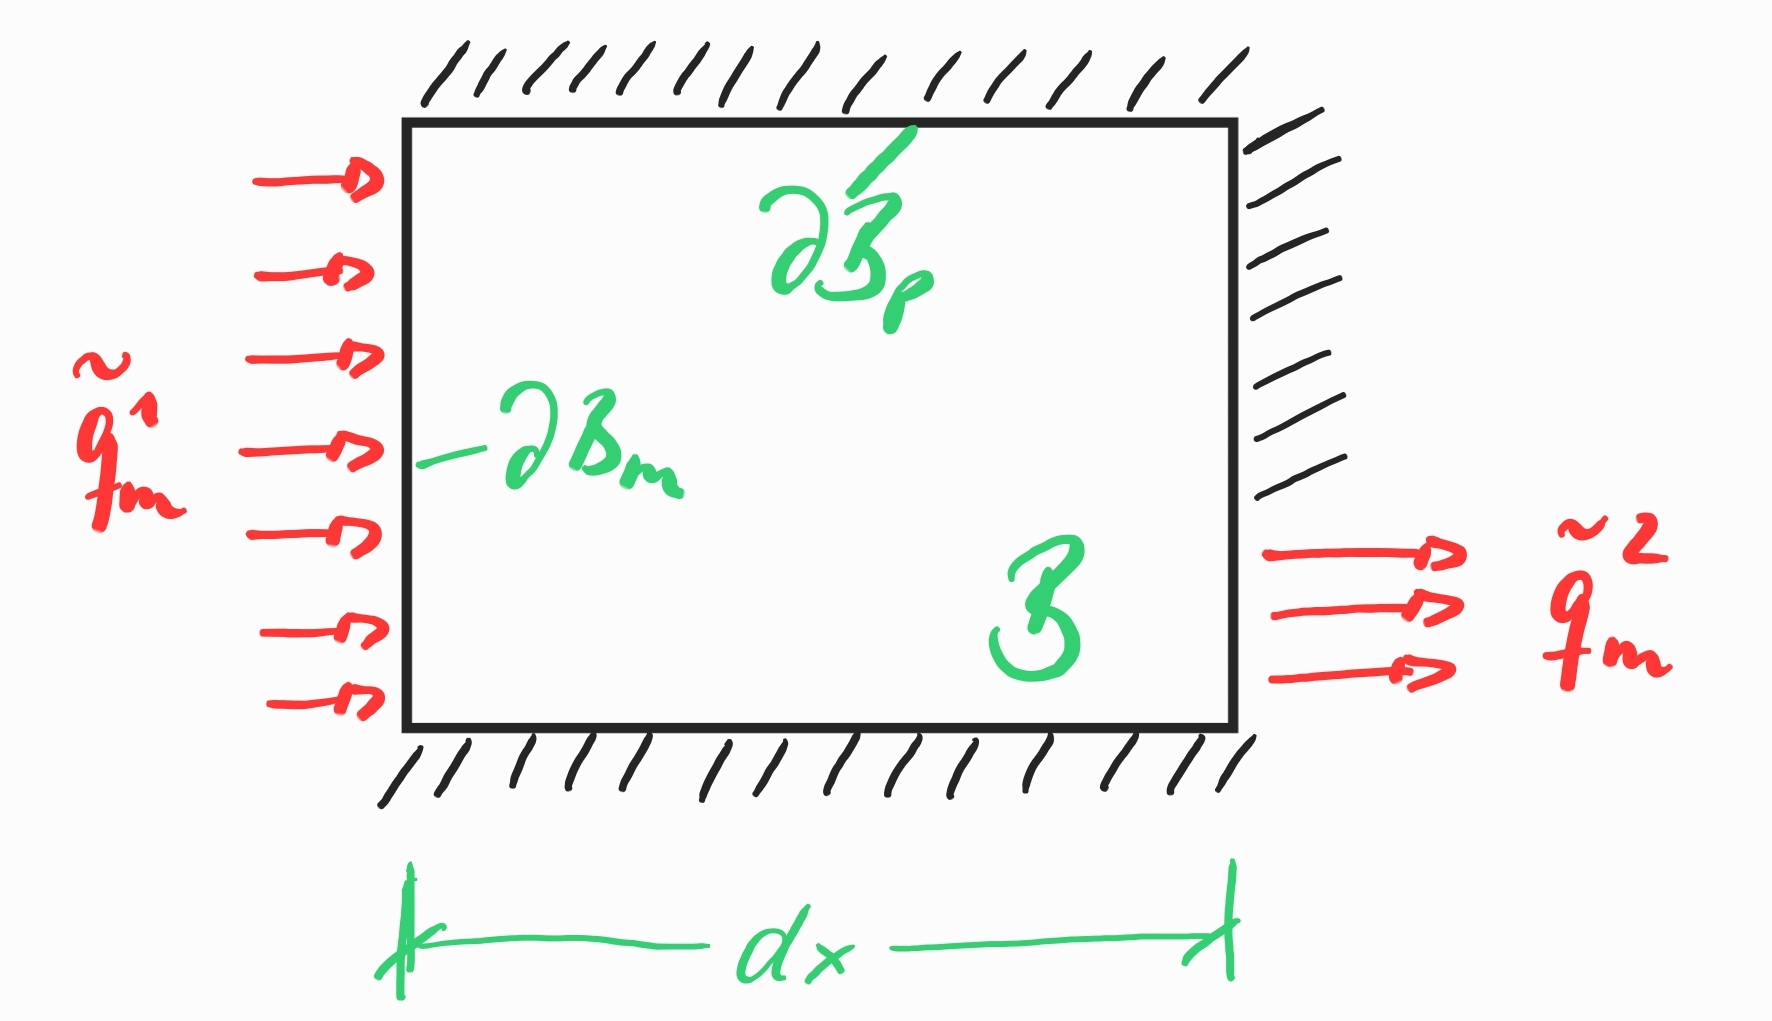
\includegraphics[width=0.7\linewidth]{files/Massenbilanz-5249ed792f311467066a05421a26a64c.jpg}
\caption[]{Ein- und Ausfluss eines infinitesimalen Volumenelementes \textbf{Austausch}}
\label{massenbilanz}
\end{figure}

Die Massenerhaltung besagt, dass die Masse eines geschlossenen Systems konstant bleibt, oder, wie in der Abbildung dargestellt, dass die zeitliche Änderung der Masse eines Systems gleich der Differenz von Zustrom und Abfluss ist. In Abwesenheit von Massenquellen oder -senken kann dies mathematisch ausgedrückt werden als:

\begin{equation}
\label{Massenbilanz}
\dot{\varrho} +  \div{\varrho {\bm{v}}} = 0
\end{equation}

Hier ist $\varrho$ die Dichte und $\bm{v}$ die Geschwindigkeit des Materials. Die zeitliche Ableitung einer Grö$\beta$e $\square$ wird durch einen Punkt über der Grö$\beta$e dargestellt: $\td{\square}$.

\begin{framed}
\textbf{Note}\\
Die Massenbilanz ist für gewöhnliche Festkörper stets erfüllt und muss nicht separat gelöst werden. Anders sieht dies im Bereich der Biomechanik oder Geomechanik aus. Hier gibt es z.B. Wachstumsprozesse (Knochen) oder Sickerströmungen. Mit der Massenbilanz kann man die Konzentration $c(\bm{x},t)$ eines Bestandteils oder den Druck $p(\bm{x},t)$ einer Phase bestimmen.
\end{framed}

Formuliert man die Massenbilanz für Fluide, dann ist die Massendichte eine Funktion des Drucks $p$, und man kann die Zeitableitung in Figure~\ref{Massenbilanz} über die Kettenregel auswerten:

\begin{equation}
\label{Massenbilanz2}
 \underbrace{\Pd{\varrho}{p}}_{=:\frac{\varrho}{\kappa}} \td{p} + \div{\varrho {\bm{v}}} = 0 \; .
\end{equation}

Die primäre Grö$\beta$e, nach der die partielle Differentialgleichung gelöst wird, ist damit der Druck $p$. Als sekundäre Grö$\beta$e bezeichnet man Feldgrö$\beta$en, die von den primären Grö$\beta$en abgeleitet sind. Im Fall der Massenbilanz des Fluids ist dies die Geschwindigkeit der Materialpartikel $\bm{v}$. Die Gleichungen Figure~\ref{Massenbilanz} und (\ref{Massenbilanz2}) beschreiben, wie sich die bilanzierte Grö$\beta$e ($p$) in der Zeit verändert; eine Information über den absoluten Wert der Grö$\beta$e erhält man erst mit der Einführung von Anfangs- und Randwerten:

\begin{align}
p(\bm{x},t=t_0) & = \tilde{p}_0 \qquad &\forall \bm{x} \in \mathcal{B}& \\
p(\bm{x},t) & = \tilde{p} \qquad &\forall \bm{x} \in \partial \mathcal{B}_p& \\
\varrho \bm{v}\T \bm{n} & = \tilde{q}_m \qquad &\forall \bm{x} \in \partial\mathcal{B}_m&
\end{align}

Hierbei wird der zweite Term auch als Dirichlet oder wesentliche Randbedingung und der dritte Term als Neumann oder natürliche Randbedingung bezeichnet.

Diese Art der mathematischen Problemstellung nennt man Anfangsrandwertproblem (IBVP - Initial Boundary Value Problem).

\begin{framed}
\textbf{IVBP1 - Massenerhaltung}\\
Bestimme das Druckfeld $p(\bm{x},t): \mathcal{B} \times [t_0,t] \rightarrow \mathcal{R}^1$, sodass für alle materiellen Punkte $\bm{x} \, \in \, \mathcal{B}$ zu jedem Zeitpunkt $t \, \in \, [t_0,t]$ die Bilanzgleichung:

\begin{equation}
\frac{\varrho}{\kappa} \td{p} + \div{\varrho {\bm{v}}} = 0
\end{equation}

unter Einhaltung der Anfangs- und Randbedingungen:

\begin{align}
p(\bm{x},t=t_0) & = \tilde{p}_0 \qquad &\forall \bm{x} \in \mathcal{B}& \\
p(\bm{x},t) & = \tilde{p} \qquad &\forall \bm{x} \in \partial \mathcal{B}_p& \\
\varrho \bm{v}\T \bm{n} & = \tilde{q}_m \qquad &\forall \bm{x} \in \partial\mathcal{B}_m&
\end{align}

erfüllt ist.
\end{framed}

%  -+-+-+-+-+-+-AI-SPLIT

\subparagraph{Impulserhaltung}

\begin{figure}[!htbp]
\centering
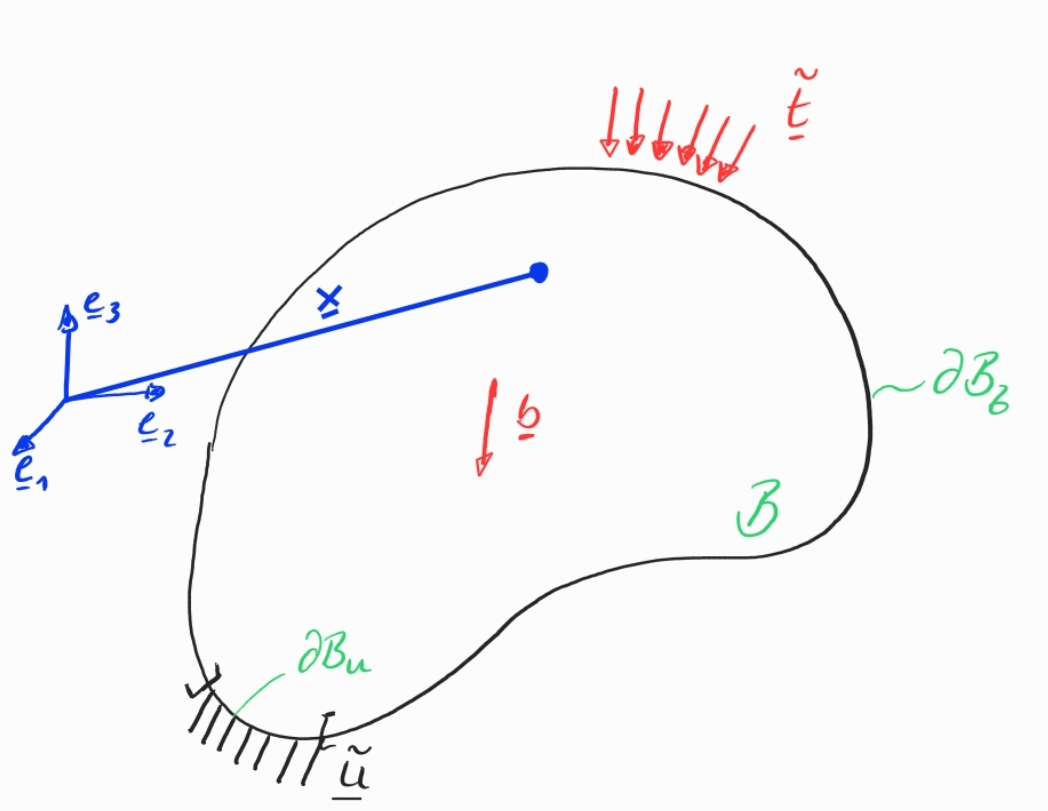
\includegraphics[width=0.7\linewidth]{files/Impulsbilanz-3c1ed32b03eec7db5f7e582ea9b4a7c5.jpg}
\caption[]{Körper $\mathcal{B}$ unter Einwirkung der externen Oberflächenkraft $\tilde{\bm{t}}$ und der Volumenlast $\bm{b}$}
\label{impulsbilanz_fig_1}
\end{figure}

Die Impulserhaltung, oft formuliert als Newtons zweites Gesetz, besagt, dass die Änderung des Impulses $\rho \bm{v}$ eines Körpers gleich der Summe der auf ihn wirkenden Kräfte ist. Für ein Kontinuum wird dies durch die Cauchy-Bewegungsgleichungen ausgedrückt:

\begin{equation}
\varrho \td{\bm{v}} =\div{\bm{\sigma}} + \rho \bm{b}
\end{equation}

$\boldsymbol{\sigma}$ steht hierbei für den Spannungstensor und $\mathbf{b}$ für die Volumenkraft pro Masseneinheit.

\begin{framed}
\textbf{Note}\\
Die Impulsbilanz ist eine vektorielle partielle Differentialgleichung. Mit ihrer Hilfe kann man das Verschiebungsfeld $\bm{u}(\bm{x},t)$ und das Spannungsfeld $\bm{\sigma}(\bm{x},t)$ eines Festkörpers bestimmen.
\end{framed}

Die primäre Feldgrö$\beta$e dieses Anfangsrandwertproblems ist die Verschiebung $\bm{u}(\bm{x},t)$ der Materialpartikel. Die sekundäre Grö$\beta$e ist die Spannung $\bm{\sigma}(\bm{x},t)$, welche wiederum von den Dehnungen $\bm{\epsilon}$ abhängig ist. Als Randwerte können entweder Verschiebungen (wesentliche Randbedingungen) vorgegeben werden oder Oberflächenspannungen (natürliche Randbedingungen).

\begin{framed}
\textbf{IVBP2 - Impulsbilanz}\\
Bestimme das Verschiebungsfeld $\bm{u}(\bm{x},t): \mathcal{B} \times [t_0,t] \rightarrow \mathcal{R}^3$, sodass für alle materiellen Punkte $\bm{x} \, \in \, \mathcal{B}$ zu jedem Zeitpunkt $t \, \in \, [t_0,t]$ die Bilanzgleichung:

\begin{equation}
\varrho \td{\bm{v}} =\div{\bm{\sigma}} + \rho \bm{b}
\end{equation}

unter Einhaltung der Anfangs- und Randbedingungen:

\begin{align}
\bm{u}(\bm{x},t=t_0) & = \tilde{\bm{u}}_0 \qquad &\forall \bm{x} \in \mathcal{B}& \\
\bm{u}(\bm{x},t) & = \tilde{\bm{u}} \qquad &\forall \bm{x} \in \partial \mathcal{B}_u& \\
\bm{\sigma}\T \bm{n} & = \tilde{\bm{t}} \qquad &\forall \bm{x} \in \partial\mathcal{B}_{\sigma}&
\end{align}

erfüllt ist.
\end{framed}

%  -+-+-+-+-+-+-AI-SPLIT

\subparagraph{Energieerhaltung}

Die Energieerhaltung stellt sicher, dass die gesamte Energie in einem abgeschlossenen System erhalten bleibt. Für ein Kontinuum kann die Energiebilanz folgenderma$\beta$en ausgedrückt werden:

\begin{equation}
\label{1HS_01}
\rho \Mtd{e} = \bm{\sigma}\T \td{\bm{\epsilon}} - \div{\bm{q}} + \varrho r
\end{equation}

Hier ist $e$ die spezifische innere Energie, $\bm{q}$ der Wärmeflussvektor und $r$ die Wärmequelle pro Masseneinheit.

\begin{framed}
\textbf{Note}\\
Die skalare Energiebilanzgleichung dient zur Berechnung des Temperaturfeldes $\theta(\bm{x},t)$.
\end{framed}

Vernachlässigt man die Kopplung zwischen Verschiebung und Temperatur, erhält man aus Gleichung (\ref{1HS_01}) die bekannte instationäre Wärmeleitungsgleichung:

\begin{equation}
\varrho c_e \Pd{\theta}{t} + \div{\bm{q}} - \varrho r = 0
\end{equation}

Hier ist die primäre Variable die Temperatur $\theta(\bm{x},t)$ und die sekundäre Variable der Wärmeflussvektor $\bm{q}(\bm{x},t)$. Gemeinsam mit den Rand- und Anfangsbedingungen erhält man das Anfangsrandwertproblem:

\begin{framed}
\textbf{IVBP3 - Energiebilanz}\\
Bestimme das Temperaturfeld $\theta(\bm{x},t): \mathcal{B} \times [t_0,t] \rightarrow \mathcal{R}^1$, sodass für alle materiellen Punkte $\bm{x} \, \in \, \mathcal{B}$ zu jedem Zeitpunkt $t \, \in \, [t_0,t]$ die Bilanzgleichung:

\begin{equation}
\varrho c_e \Pd{\theta}{t} + \div{\bm{q}} - \varrho r = 0
\end{equation}

unter Einhaltung der Anfangs- und Randbedingungen:

\begin{align}
\theta(\bm{x},t=t_0) & = \tilde{\theta}_0 \qquad &\forall \bm{x} \in \mathcal{B}& \\
\theta(\bm{x},t) & = \tilde{\theta} \qquad &\forall \bm{x} \in \partial \mathcal{B}_{\theta}& \\
\bm{q}\T \bm{n} & = \tilde{\bm{q}} \qquad &\forall \bm{x} \in \partial\mathcal{B}_q&
\end{align}

erfüllt ist.
\end{framed}

%  -+-+-+-+-+-+-AI-SPLIT

\subparagraph{Zusammenfassung}

In den vorangegangenen Abschnitten wurden die Bilanzgleichungen der Kontinuumsmechanik verwendet, um die für die Ingenieurpraxis wichtigen Anfangsrandwertprobleme der Fluid-, Struktur- und Thermomechanik aufzustellen. Für diese Systeme von gekoppelten partiellen Differentialgleichungen gibt es nur in wenigen Sonderfällen analytische Lösungen. Einige davon sind uns aus den Vorlesungen zur Elastostatik und Strömungslehre bekannt. Aus diesem Grund haben sich numerische Berechnungsverfahren durchgesetzt. Um zu überprüfen, ob die Anfangsrandwertprobleme in der obigen Form lösbar sind, werden in der nachfolgenden Tabelle die Bestimmungsgleichungen und die Unbekannten gegenübergestellt.

\bigskip\noindent
\begin{tabular}{p{\dimexpr 0.200\linewidth-2\tabcolsep}p{\dimexpr 0.200\linewidth-2\tabcolsep}p{\dimexpr 0.200\linewidth-2\tabcolsep}p{\dimexpr 0.200\linewidth-2\tabcolsep}p{\dimexpr 0.200\linewidth-2\tabcolsep}}
\toprule
Bestimmungsgleichung & Anzahl an Gleichungen & Unbekannte & Anzahl an Unbekannten & Anzahl an zusätzlichen Bedingungen \\
\hline
Massenbilanz & 1 & $p$, $\bm{v}$ & 4 & 3 \\
Impulsbilanz & 3 & $\bm{u}$, $\bm{\sigma}$, $\bm{\epsilon}$ & 15 & 12 \\
Energiebilanz & 1 & $\theta$, $\bm{q}$ & 4 & 3 \\
\bottomrule
\end{tabular}

\bigskip Wie leicht zu erkennen ist, genügt die Anzahl an Gleichungen für keines der obigen Probleme zur Lösung. Es werden darum zusätzliche Bedingungen formuliert, um die Anfangsrandwertprobleme zu lösen:

\begin{itemize}
\item Kinematische Bedingungen
\item Materialmodelle
\end{itemize}

%  -+-+-+-+-+-+-AI-SPLIT

\paragraph{Kinematik}

Kinematische Bedingungen spielen besonders im Bereich der Strukturmechanik und der Lösung der Impulsbilanz eine herausragende Rolle. Ein Beispiel hierfür ist die Forderung nach dem Ebenbleiben des Querschnitts in der Bernoulli-Balkentheorie, die zu der bekannten Differentialgleichung der Durchbiegung $w(x)$ führt.
In der linearen Kontinuumsmechanik wird die Dehnung $\bm{\epsilon}$ als der symmetrische Anteil des Verschiebungsgradienten $\grad{\bm{u}}$ betrachtet:

\begin{equation}
\label{linearStrain}
\bm{\epsilon} = \frac{1}{2} \left(\grad{\bm{u}}\T + \grad{\bm{u}} \right) \; .
\end{equation}

Dieses Dehnungsma$\beta$ wird oft auch als Ingenieurdehnung bezeichnet und sollte nur in einem Dehnungsbereich von weniger als 10\% angewendet werden. Zudem ist hervorzuheben, dass Starrkörpertranslationen keine Ingenieurdehnung verursachen, Starrkörperrotationen hingegen sehr wohl. Aus diesem Grund ist darauf zu achten, dass beim Auftreten grö$\beta$erer Rotationen stets eine nichtlineare Theorie (2. Ordnung oder allgemein nichtlinear) verwendet wird.

Aufgrund der Symmetrie des Dehnungstensors erhalten wir \textbf{6} zusätzliche Bedingungen zur Lösung des Anfangsrandwertproblems der Impulsbilanz.

\paragraph{Materialmodell}

Was zur Schlie$\beta$ung der mathematischen Problemstellung jetzt noch fehlt, ist eine Relation zwischen der primären Feldgrö$\beta$e und ihrer zugeordneten Flussgrö$\beta$e (sekundäre Grö$\beta$e). Die oben beschriebenen Bilanzgleichungen sind physikalische Prinzipien, die unabhängig vom Werkstoff Gültigkeit besitzen. Die spezifischen Werkstoffeigenschaften werden über Materialmodelle, sogenannte konstitutive Modelle, in das Anfangsrandwertproblem eingebracht. Die konstitutive Materialtheorie ist eine Wissenschaft für sich und soll in dieser Vorlesung nicht weiter behandelt werden. In der Strukturmechanik können Materialien entsprechend ihrer Eigenschaften in folgende Klassen eingeteilt werden:

\begin{figure}[!htbp]
\centering
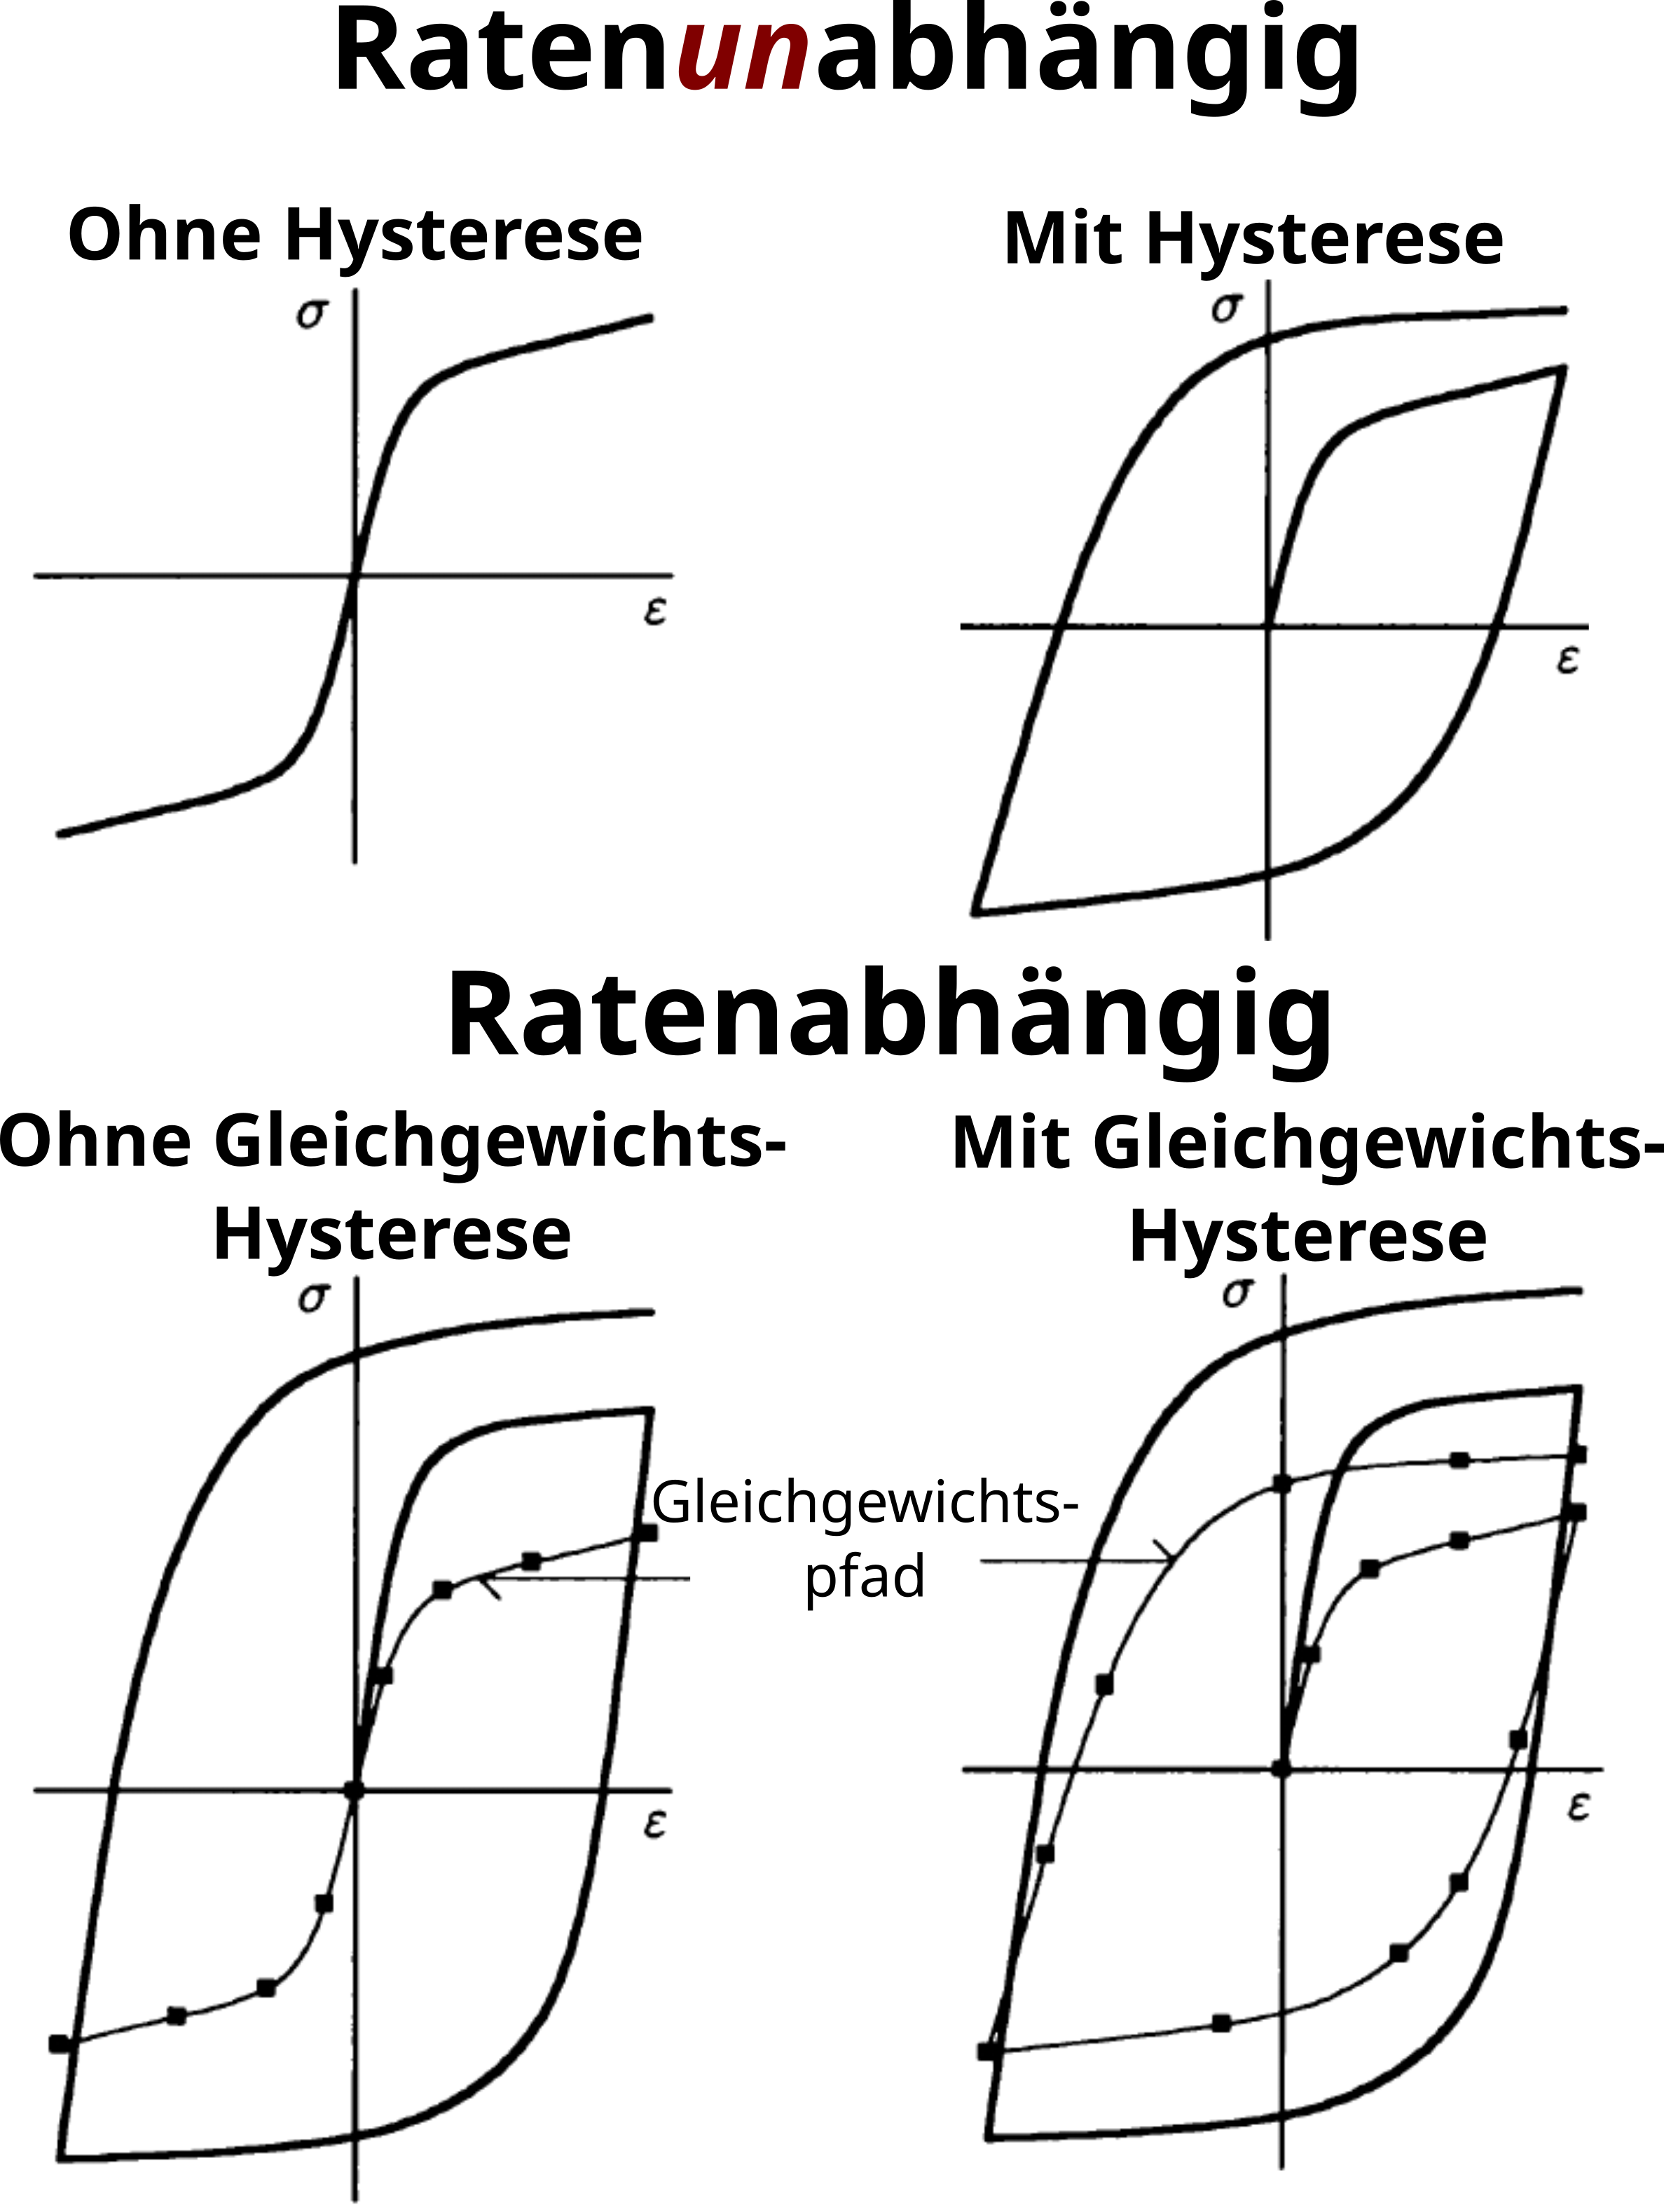
\includegraphics[width=0.7\linewidth]{files/Materialklassen-0654260d23db48934efafd3d240353a4.png}
\caption[]{Klassifizierung von Materialmodellen anhand ihrer Systemantwort. Abbildung nach \cite{haupt2013continuum}}
\label{materialklassen}
\end{figure}

%  -+-+-+-+-+-+-AI-SPLIT

\subparagraph{Wärmeleitung}

Bei der Berechnung der Wärmeleitungsgleichung wird oftmals die \textbf{Fourier}sche Wärmeleitung zugrunde gelegt. Diese basiert auf der Annahme, dass der Wärmestrom proportional zum negativen Temperaturgradienten ist:

\begin{equation}
\label{fourier}
\bm{q} = - \bm{k}\T  \grad{\theta} \, .
\end{equation}
Hierbei ist $\bm{k}$ der Konduktivitätstensor, welcher für isotrope Materialien wie folgt aussieht:
\begin{equation}
\label{konduktivitaetsmatrixIsotrop}
 \bm{k} = k \begin{bmatrix} 1 & 0 & 0 \\ 0 & 1 & 0 \\ 0 & 0 & 1\end{bmatrix}  \, ,
\end{equation}
mit der Wärmeleitfähigkeit $k$ in $\frac{\text{W}}{\text{m}\cdot\text{K}}$. Der Wärmestromvektor hat damit die Einheit $\frac{\text{W}}{\text{m}^2}$.

\begin{framed}
\textbf{Zusätzliche Gleichungen}\\
Aus Gleichung (\ref{fourier}) erhalten wir \textbf{3} zusätzliche Gleichungen. Wir haben jetzt genauso viele Gleichungen wie Unbekannte.
\end{framed}

\begin{framed}
\textbf{Materialsymmetrie (Auswahl)}\\
\begin{itemize}
\item isotrop - gleiche Eigenschaften in alle Raumrichtungen
\item transversal isotrop - unterschiedliche Eigenschaften entlang einer Faser (Symmetrieachse) und der zu dieser Faser senkrecht stehenden Ebene
\item orthotrop - drei paarweise senkrecht zueinander stehende Symmetrieachsen
\end{itemize}
\end{framed}

%  -+-+-+-+-+-+-AI-SPLIT

\subparagraph{Durchströmung}

Bei der Berechnung der Fluidgeschwindigkeit in Sickerströmungen wird oftmals das \textbf{Darcy}sche hydraulische Strömungsgesetz angewendet. Dies ist analog zur Wärmeleitung definiert als proportional zum negativen Druckgradienten:

\begin{equation}
\label{darcy}
\bm{v} = - \bm{k}_{\varepsilon}\T  \grad{p} \, .
\end{equation}
Hierbei ist $\bm{k}_{\varepsilon}$ die hydraulische Konduktivität. Für isotrope Materialien gilt:

\begin{equation}
 \bm{k}_{\varepsilon} = \frac{k_{\varepsilon}}{\mu} \begin{bmatrix} 1 & 0 & 0 \\ 0 & 1 & 0 \\ 0 & 0 & 1\end{bmatrix}  \, ,
\end{equation}
mit der hydraulischen Permeabilität $k_{\varepsilon}$ in $\text{m}^2$ und der dynamischen Viskosität $\mu$ in $\text{Pa}\cdot \text{s}$.

\begin{framed}
\textbf{Zusätzliche Gleichungen}\\
Aus Gleichung (\ref{darcy}) erhalten wir \textbf{3} zusätzliche Gleichungen. Wir haben jetzt genauso viele Gleichungen wie Unbekannte.
\end{framed}

%  -+-+-+-+-+-+-AI-SPLIT

\subparagraph{Lineare Elastizität}

In Figure~\ref{materialklassen} sind verschiedene Klassen von Festkörpermaterialien dargestellt. In dieser Vorlesung behandeln wir lediglich eine Unterklasse der ratenunabhängigen Materialien ohne Hysterese. Die lineare Elastizität ist gekennzeichnet durch einen linearen Zusammenhang zwischen Spannung $\bm{\sigma}$ und Dehnungen $\bm{\epsilon}$. In tensorieller Notation stellt sich das verallgemeinerte Hooke'sche Gesetz wie folgt dar:

\begin{equation}
\label{generalHook}
\sigma_{ij} = \mathbb{C}_{ijkl} \epsilon_{kl} \;
\end{equation}

wobei von der Einsteinschen Summenkonvention Gebrauch gemacht wurde. In der Strukturmechanik ist es jedoch unüblich, mit Tensoren 4. Stufe explizit zu rechnen. Es werden Symmetrieeigenschaften der Tensoren $\sigma_{ij}=\sigma_{ji}$, $\epsilon_{ij}=\epsilon_{ji}$ und $\mathbb{C}_{ijkl}=\mathbb{C}_{klij}$ ausgenutzt, um Tensorprodukte wie z.B. in Gleichung (\ref{generalHook}) in Matrix-Vektor-Operationen zu überführen. Dies ist vor allem für die numerische Implementierung von gro$\beta$em Vorteil.

\begin{equation}
\label{generalHook2}
\begin{bmatrix} 
\sigma_{11} \\
\sigma_{22} \\
\sigma_{33} \\
\sigma_{12} \\
\sigma_{23} \\
\sigma_{13} 
\end{bmatrix} = \begin{bmatrix}
C_{1111} & C_{1122} & C_{1133} & C_{1112} & C_{1123} & C_{1113} \\
C_{2211} & C_{2222} & C_{2233} & C_{2212} & C_{2223} & C_{2213} \\
C_{3311} & C_{3322} & C_{3333} & C_{3312} & C_{3323} & C_{3313} \\
C_{1211} & C_{1222} & C_{1233} & C_{1212} & C_{1223} & C_{1213} \\
C_{2311} & C_{2322} & C_{2333} & C_{2312} & C_{2323} & C_{2313} \\
C_{1311} & C_{1322} & C_{1333} & C_{1312} & C_{1323} & C_{1313} \\ 
\end{bmatrix} \begin{bmatrix} \epsilon_{11} \\ \epsilon_{22} \\ \epsilon_{33} \\ 2\epsilon_{12} \\ 2\epsilon_{23} \\ 2\epsilon_{13} \end{bmatrix}
\end{equation}

Für isotrope lineare Elastizität mit den Materialkonstanten:

\begin{itemize}
\item $E$ - Elastizitätsmodul in $\text{MPa}$
\item $\nu$ - Querkontraktionszahl in [-]
\end{itemize}

erhält man dann:

\begin{equation}
\label{generalHook3}
\begin{bmatrix} 
\sigma_{11} \\
\sigma_{22} \\
\sigma_{33} \\
\sigma_{12} \\
\sigma_{23} \\
\sigma_{13} 
\end{bmatrix} = \frac{E}{(1+\nu)(1-2\nu)}\begin{bmatrix}
1-\nu & \nu & \nu & 0 & 0 & 0 \\
\nu & 1-\nu & \nu & 0 & 0 & 0 \\
\nu & \nu & 1-\nu & 0 & 0 & 0 \\
0 & 0 & 0 & \frac{1-2\nu}{2} & 0 & 0 \\
0 & 0 & 0 & 0 & \frac{1-2\nu}{2} & 0 \\
0 & 0 & 0 & 0 & 0 & \frac{1-2\nu}{2} \\ 
\end{bmatrix} \begin{bmatrix} \epsilon_{11} \\ \epsilon_{22} \\ \epsilon_{33} \\ 2\epsilon_{12} \\ 2\epsilon_{23} \\ 2\epsilon_{13} \end{bmatrix}
\end{equation}

Für die inverse Beziehung $\bm{\epsilon} = \bm{C}^{ -1} \bm{\sigma}$ mit der Nachgiebigkeitsmatrix $\bm{C}^{ -1}$ erhält man:
\begin{equation}
\label{generalHook4}
\begin{bmatrix} 
\epsilon_{11} \\
\epsilon_{22} \\
\epsilon_{33} \\
2\epsilon_{12} \\
2\epsilon_{23} \\
2\epsilon_{13} 
\end{bmatrix} =\begin{bmatrix}
\frac{1}{E} & \frac{-\nu}{E} & \frac{-\nu}{E} & 0 & 0 & 0 \\
\frac{-\nu}{E} & \frac{1}{E} & \frac{-\nu}{E} & 0 & 0 & 0 \\
\frac{-\nu}{E} & \frac{-\nu}{E} & \frac{1}{E} & 0 & 0 & 0 \\
0 & 0 & 0 & \frac{1}{G} & 0 & 0 \\
0 & 0 & 0 & 0 & \frac{1}{G} & 0 \\
0 & 0 & 0 & 0 & 0 & \frac{1}{G} \\ 
\end{bmatrix} \begin{bmatrix} \sigma_{11} \\ \sigma_{22} \\ \sigma_{33} \\ \sigma_{12} \\ \sigma_{23} \\ \sigma_{13} \end{bmatrix}
\end{equation}

wobei $G=\frac{E}{2(1+\nu)}$ den Schubmodul in $\text{MPa}$ darstellt.

\begin{framed}
\textbf{Zusätzliche Gleichungen}\\
Aus Gleichung (\ref{generalHook3}) und (\ref{generalHook4}) erhalten wir \textbf{6} zusätzliche Gleichungen. Wir haben jetzt genauso viele Gleichungen wie Unbekannte.
\end{framed}

%  -+-+-+-+-+-+-AI-SPLIT

\begin{framed}
\textbf{Einsteinsche Summenkonvention}\\
Die Einsteinsche Summenkonvention ist eine Notationsvereinbarung, die in der Tensorrechnung verwendet wird, um Ausdrücke zu vereinfachen. Wenn ein Index in einem mathematischen Ausdruck zweimal vorkommt, wird implizit über diesen Index summiert:

\begin{equation}
c_i = \sum_{j=1}^{n} a_{ij} b_j \qquad \rightarrow \qquad  c_i=a_{ij} b_j
\end{equation}
\end{framed}

\begin{framed}
\textbf{Kelvin-Notation vs. Voigt-Notation}\\
Die Kelvin-Notation und die Voigt-Notation sind zwei verschiedene Methoden, um tensorielle Grö$\beta$en in Matrix- und Vektorschreibweise zu überführen. In den meisten kommerziellen FEM-Programmen ist die Voigt-Notation vorzufinden, wobei neuere FE-Codes durchaus die Vorteile der Kelvin-Notation ausnutzen \cite{nagel2016advantages}. Allgemein kann gesagt werden, dass die Voigt-Notation näher an der Ingenieurmechanik ist, da die Scheranteile $\epsilon_{ij} \quad \forall i\neq j$ der Dehnung doppelt eingehen und wir somit die Gleitungen $\gamma_{ij} \quad \forall i\neq j$ erhalten. Die Kelvin-Notation hat den Vorteil, dass mit ihr weiterhin alle Tensorprodukte einfach gebildet werden können, ohne dass über den Vorfaktor der Komponenten nachgedacht werden muss. Im aktuellen Kurs wird die \textbf{Voigt}-Notation zugrunde gelegt.

\bigskip\noindent
\begin{tabular}{p{\dimexpr 0.500\linewidth-2\tabcolsep}p{\dimexpr 0.500\linewidth-2\tabcolsep}}
\toprule
 & Voigt-Notation \\
\hline
$\sigma_{ij}$ & $\bm{\sigma}= \begin{bmatrix} \sigma_{11} & \sigma_{22} & \sigma_{33} & \sigma_{12} & \sigma_{23} & \sigma_{13} \end{bmatrix}\T$ \\
$\epsilon_{ij}$ & $\bm{\epsilon}= \begin{bmatrix} \epsilon_{11} & \epsilon_{22} & \epsilon_{33} & 2\epsilon_{12} & 2\epsilon_{23} & 2\epsilon_{13} \end{bmatrix}\T$ \\
$\sigma_{ij}=\mathbb{C}_{ijkl}\epsilon_{kl}$ & $\bm{\sigma} = \bm{C} \bm{\epsilon}$ \\
$\mathcal{E}=\sigma_{ij}\epsilon_{ij}$ & $\mathcal{E} = \bm{\sigma}\T\bm{\epsilon}$ \\
\bottomrule
\end{tabular}

\bigskip\begin{equation}
\mathbb{C}_{ijkl} \quad \rightarrow \quad \bm{C}=\begin{bmatrix}
C_{1111} & C_{1122} & C_{1133} & C_{1112} & C_{1123} & C_{1113} \\
C_{2211} & C_{2222} & C_{2233} & C_{2212} & C_{2223} & C_{2213} \\
C_{3311} & C_{3322} & C_{3333} & C_{3312} & C_{3323} & C_{3313} \\
C_{1211} & C_{1222} & C_{1233} & C_{1212} & C_{1223} & C_{1213} \\
C_{2311} & C_{2322} & C_{2333} & C_{2312} & C_{2323} & C_{2313} \\
C_{1311} & C_{1322} & C_{1333} & C_{1312} & C_{1323} & C_{1313} \\ 
\end{bmatrix}
\end{equation}

\bigskip\noindent
\begin{tabular}{p{\dimexpr 0.500\linewidth-2\tabcolsep}p{\dimexpr 0.500\linewidth-2\tabcolsep}}
\toprule
 & Kelvin-Notation \\
\hline
$\sigma_{ij}$ & $\bm{\sigma}= \begin{bmatrix} \sigma_{11} & \sigma_{22} & \sigma_{33} & \sqrt{2}\sigma_{12} & \sqrt{2}\sigma_{23} & \sqrt{2}\sigma_{13} \end{bmatrix}\T$ \\
$\epsilon_{ij}$ & $\bm{\epsilon}= \begin{bmatrix} \epsilon_{11} & \epsilon_{22} & \epsilon_{33} & \sqrt{2}\epsilon_{12} & \sqrt{2}\epsilon_{23} & \sqrt{2}\epsilon_{13} \end{bmatrix}\T$ \\
$\sigma_{ij}=\mathbb{C}_{ijkl}\epsilon_{kl}$ & $\bm{\sigma} = \bm{C} \bm{\epsilon}$ \\
$\mathcal{E}=\sigma_{ij}\epsilon_{ij}$ & $\mathcal{E} = \bm{\sigma}\T\bm{\epsilon}$ \\
\bottomrule
\end{tabular}

\bigskip\begin{equation}
\mathbb{C}_{ijkl} \quad \rightarrow \quad \bm{C}=\begin{bmatrix}
C_{1111} & C_{1122} & C_{1133} & \sqrt{2}C_{1112} & \sqrt{2}C_{1123} & \sqrt{2}C_{1113} \\
C_{2211} & C_{2222} & C_{2233} & \sqrt{2}C_{2212} & \sqrt{2}C_{2223} & \sqrt{2}C_{2213} \\
C_{3311} & C_{3322} & C_{3333} & \sqrt{2}C_{3312} & \sqrt{2}C_{3323} & \sqrt{2}C_{3313} \\
\sqrt{2}C_{1211} & \sqrt{2}C_{1222} & \sqrt{2}C_{1233} & 2C_{1212} & 2C_{1223} & 2C_{1213} \\
\sqrt{2}C_{2311} & \sqrt{2}C_{2322} & \sqrt{2}C_{2333} & 2C_{2312} & 2C_{2323} & 2C_{2313} \\
\sqrt{2}C_{1311} & \sqrt{2}C_{1322} & \sqrt{2}C_{1333} & 2C_{1312} & 2C_{1323} & 2C_{1313} \\ 
\end{bmatrix}
\end{equation}
\end{framed}

%  -+-+-+-+-+-+-AI-SPLIT

\subparagraph{Ebener Verzerrungszustand}

\begin{figure}[!htbp]
\centering
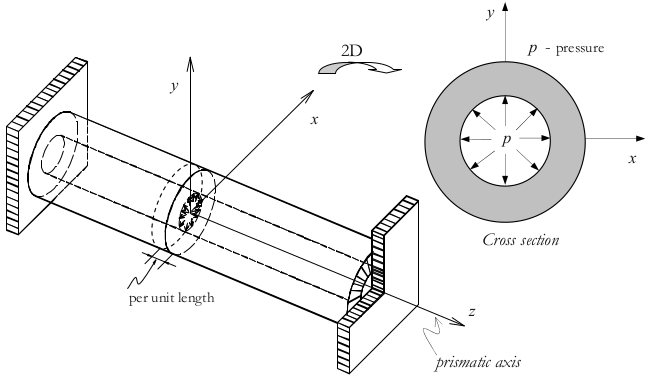
\includegraphics[width=0.7\linewidth]{files/EVZ-d6cb9ec161125a880d46ccc9573e94fb.png}
\caption[]{Beispiel für das Auftreten eines ebenen Verzerrungszustands \cite{chaves2013notes}}
\label{evz}
\end{figure}

Betrachten wir ein Strukturelement mit prismatischen Merkmalen, bei dem die Dimension in Richtung der prismatischen Achse deutlich grö$\beta$er ist als die anderen Dimensionen. Die aufgebrachten Lasten wirken senkrecht zur prismatischen Achse (Figure~\ref{evz}). Unter diesen Bedingungen sind die Dehnungskomponenten $\e_{13},\, \e_{23}, \, \e_{33}$ gleich null. Dieser Zustand wird als ebener Verzerrungszustand bezeichnet. Beispiele hierfür sind Stützmauern, unter Druck stehende Zylinder, Dämme, Tunnel und Flachgründungen.

Es muss betont werden, dass die Variablen (Last, Querschnitt, Material) entlang der prismatischen Achse konstant sein müssen, um einen ebenen Verzerrungszustand zu betrachten. Andernfalls können erhebliche Fehler auftreten.

\begin{framed}
\textbf{Prismatische Merkmale}\\
\begin{itemize}
\item Konstanter Querschnitt entlang der Längsachse
\item Längliche Form
\item Geradlinige Achse
\end{itemize}

\textbf{Beispiele:} Balken, Säulen, Rohre
\end{framed}

Um die konstitutive Beziehung $\sb(\eb)$ zu erhalten, starten wir vom generalisierten Hook'schen Gesetz (\ref{generalHook3}), indem wir alle Spalten mit korrespondierenden 0-Dehnungen eliminieren:

\begin{equation}
\label{evz1}
\begin{bmatrix} 
\sigma_{11} \\
\sigma_{22} \\
\sigma_{33} \\
\sigma_{12} \\
\sigma_{23} \\
\sigma_{13} 
\end{bmatrix} = \frac{E}{(1+\nu)(1-2\nu)}\begin{bmatrix}
1-\nu & \nu & \cancel{\nu} & 0 & \cancel{0} & \cancel{0} \\
\nu & 1-\nu & \cancel{\nu} & 0 & \cancel{0} & \cancel{0} \\
\nu & \nu & \cancel{1-\nu} & 0 & \cancel{0} & \cancel{0} \\
0 & 0 & \cancel{0} & \frac{1-2\nu}{2} & \cancel{0} & \cancel{0} \\
0 & 0 & \cancel{0} & 0 & \cancel{\frac{1-2\nu}{2}} & \cancel{0} \\
0 & 0 & \cancel{0} & 0 & \cancel{0} & \cancel{\frac{1-2\nu}{2}} \\ 
\end{bmatrix} \begin{bmatrix} \epsilon_{11} \\ \epsilon_{22} \\ \cancel{\epsilon_{33}} \\ 2\epsilon_{12} \\ \cancel{2\epsilon_{23}} \\ \cancel{2\epsilon_{13}} \end{bmatrix}
\end{equation}

Wir sehen sofort, dass die Komponenten $\s_{23},\, \s_{13}$ verschwinden. Die Spannungskomponente entlang der prismatischen Achse $\s_{33}$ hingegen berechnet sich zu:

\begin{equation}
\s_{33} = \frac{E \nu}{(1+\nu)(1-2\nu)} \left(\e_{11} + \e_{22} \right)
\end{equation}

%  -+-+-+-+-+-+-AI-SPLIT

Arrangiert man die verbleibenden Einträge, so erhält man für $\bm{C}\rs{EVZ}$:
\begin{equation}
\label{evz2}
 \begin{bmatrix} 
\s_{11} \\
\s_{22} \\
\s_{12} 
\end{bmatrix}= \underbrace{\frac{E }{(1+\nu)(1-2\nu)} \begin{bmatrix}
1-\nu & \nu & 0 \\
\nu & 1-\nu & 0 \\
0 & 0 & \frac{1-2\nu}{2}
\end{bmatrix}}_{\bm{C}\rs{EVZ}}  \begin{bmatrix} 
\e_{11} \\
\e_{22} \\
\e_{12} 
\end{bmatrix}
\end{equation}

Für die Nachgiebigkeit $\bm{C}\rs{EVZ}^{ -1}$ erhält man die inverse Beziehung:
\begin{equation}
\label{evz3}
 \begin{bmatrix} 
\e_{11} \\
\e_{22} \\
\e_{12} 
\end{bmatrix}= \underbrace{\frac{1+\nu }{E} \begin{bmatrix}
1-\nu & -\nu & 0 \\
-\nu & 1-\nu & 0 \\
0 & 0 & 2
\end{bmatrix}}_{\bm{C}\rs{EVZ}^{-1}}  \begin{bmatrix} 
\s_{11} \\
\s_{22} \\
\s_{12} 
\end{bmatrix}
\end{equation}

%  -+-+-+-+-+-+-AI-SPLIT

\subparagraph{Ebener Spannungszustand}

\begin{figure}[!htbp]
\centering
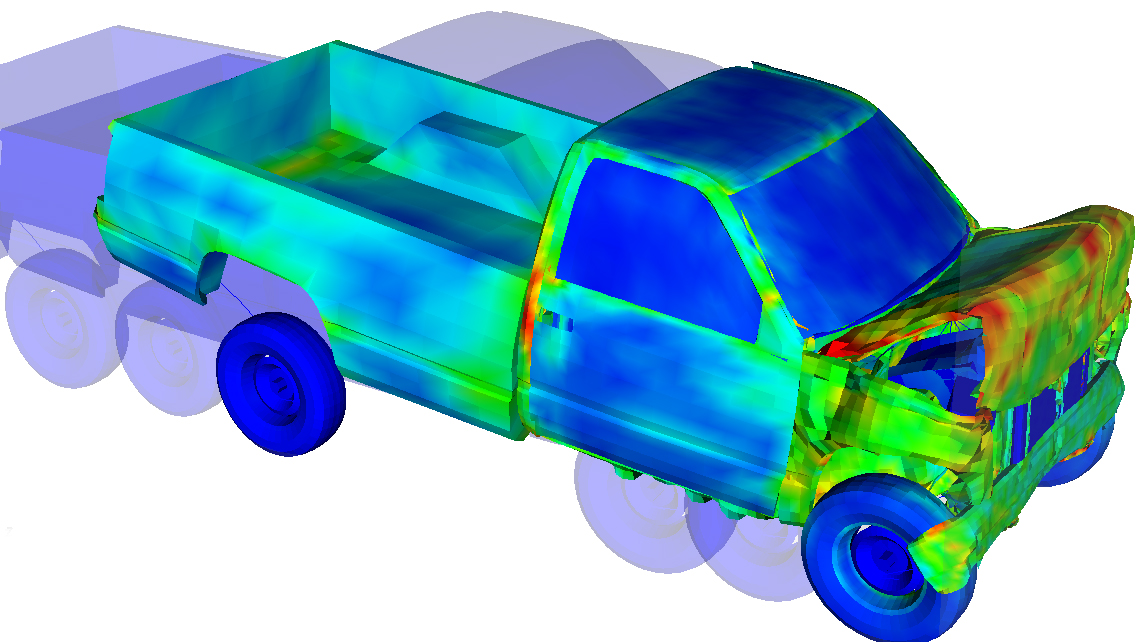
\includegraphics[width=0.7\linewidth]{files/CarCrash-dbcc46180747582567a8cdb800f7cc04.jpg}
\caption[]{FEM Crash-Simulation eines Pickup-Trucks gegen eine starre Wand \href{https://enteknograte.com/wp-content/uploads/2022/06/truck-crash-Car-vehicle-Finite-Element-Simulation-Crash-Test-MSC-dytran-Crashworthiness-Ls-Dyna-Abaqus-PAM-CRASH.jpg}{Quelle}}
\label{carcrash}
\end{figure}

Der ebene Spannungszustand tritt überall dort auf, wo Flächenelemente vor allem in ihrer Ebene belastet werden und die Flächenabmessungen deutlich grö$\beta$er sind als die dazugehörige Dicke. Dies ist zum Beispiel bei Karosserieblechen, wie in Figure~\ref{carcrash}, der Fall.

\begin{figure}[!htbp]
\centering
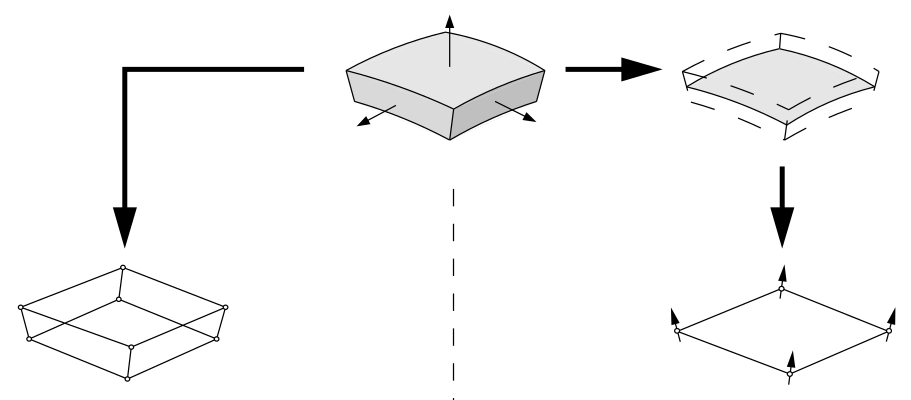
\includegraphics[width=0.7\linewidth]{files/Shellformulation-69f62cd7489fe0ebc779931fdd28af92.png}
\caption[]{FEM-Diskretisierung von Schalenelementen als degenerierte Volumenelemente (links) oder über eine Mittelflächendarstellung (rechts). \cite{wriggers2008nonlinear}}
\label{shellformulation}
\end{figure}

In Abbildung Figure~\ref{shellformulation} auf der rechten Seite ist eine Diskretisierung für den ebenen Spannungszustand mit Mittelflächenelementen zu sehen.

Startpunkt für die konstitutive Beziehung ist die Gleichung (\ref{generalHook4}). Zunächst streichen wir alle Spalten, die den 0-Spannungen zugeordnet werden können:
\begin{equation}
\label{generalHookESZ1}
\begin{bmatrix} 
\epsilon_{11} \\
\epsilon_{22} \\
\epsilon_{33} \\
2\epsilon_{12} \\
2\epsilon_{23} \\
2\epsilon_{13} 
\end{bmatrix} = \begin{bmatrix}
\frac{1}{E} & \frac{-\nu}{E} & \cancel{\frac{-\nu}{E}} & 0 & \cancel{0} & \cancel{0} \\
\frac{-\nu}{E} & \frac{1}{E} & \cancel{\frac{-\nu}{E}} & 0 & \cancel{0} & \cancel{0} \\
{\frac{-\nu}{E}} & {\frac{-\nu}{E}} & \cancel{\frac{1}{E}} & {0} & \cancel{0} & \cancel{0} \\
0 & 0 & \cancel{0} & \frac{1}{G} & 0 & 0 \\
{0} & {0} & \cancel{0} & {0} & \cancel{\frac{1}{G}} & \cancel{0} \\
{0} & {0} & \cancel{0} & {0} & \cancel{0} & \cancel{\frac{1}{G}} \\ 
\end{bmatrix} \begin{bmatrix} \sigma_{11} \\ \sigma_{22} \\ \cancel{\sigma_{33}} \\ \sigma_{12} \\ \cancel{\sigma_{23}} \\ \cancel{\sigma_{13}} \end{bmatrix}
\end{equation}

Hier fällt auf, dass das resultierende System nicht mehr quadratisch ist, da die Dehnung in Dickenrichtung $\epsilon_{33}$ ungleich null ist:

\begin{equation}
\label{generalHookESZ2}
\begin{bmatrix} 
\epsilon_{11} \\
\epsilon_{22} \\
\epsilon_{33} \\
2\epsilon_{12} \\
\end{bmatrix} = \begin{bmatrix}
\frac{1}{E} & \frac{-\nu}{E}  & 0  \\
\frac{-\nu}{E} & \frac{1}{E}  & 0  \\
{\frac{-\nu}{E}} & {\frac{-\nu}{E}} & {0} \\
0 & 0 & \frac{1}{G}  \\
\end{bmatrix} \begin{bmatrix} \sigma_{11} \\ \sigma_{22} \\ \sigma_{12} \end{bmatrix} \; .
\end{equation}

Dieses System hat eine Gleichung zu viel. Zweckmä$\beta$ig vernachlässigt man die Gleichung für die Dehnung in Dickenrichtung (diese Dehnung berechnet man in einer Nachlaufrechnung). Somit lautet die Nachgiebigkeitsmatrix $\bm{C}^{ -1}\rs{ESZ}$ und die materielle Steifigkeitsmatrix $\bm{C}\rs{ESZ}$ für den ebenen Spannungszustand:

\begin{equation}
\label{generalHookESZ3}
\bm{C}^{-1} = \frac{1}{E} \begin{bmatrix}
1 & -\nu & 0  \\
-\nu & 1  & 0  \\
0 & 0 & 2(1+\nu)  \\
\end{bmatrix}  \qquad 
\bm{C} = \frac{E}{(1-\nu^2)}\begin{bmatrix}
1 & \nu  & 0  \\
\nu & 1  & 0  \\
0 & 0 & \frac{1-\nu}{2}  \\
\end{bmatrix}
\end{equation}

%  -+-+-+-+-+-+-AI-SPLIT

\subparagraph{Rotationssymmetrie}

\begin{figure}[!htbp]
\centering
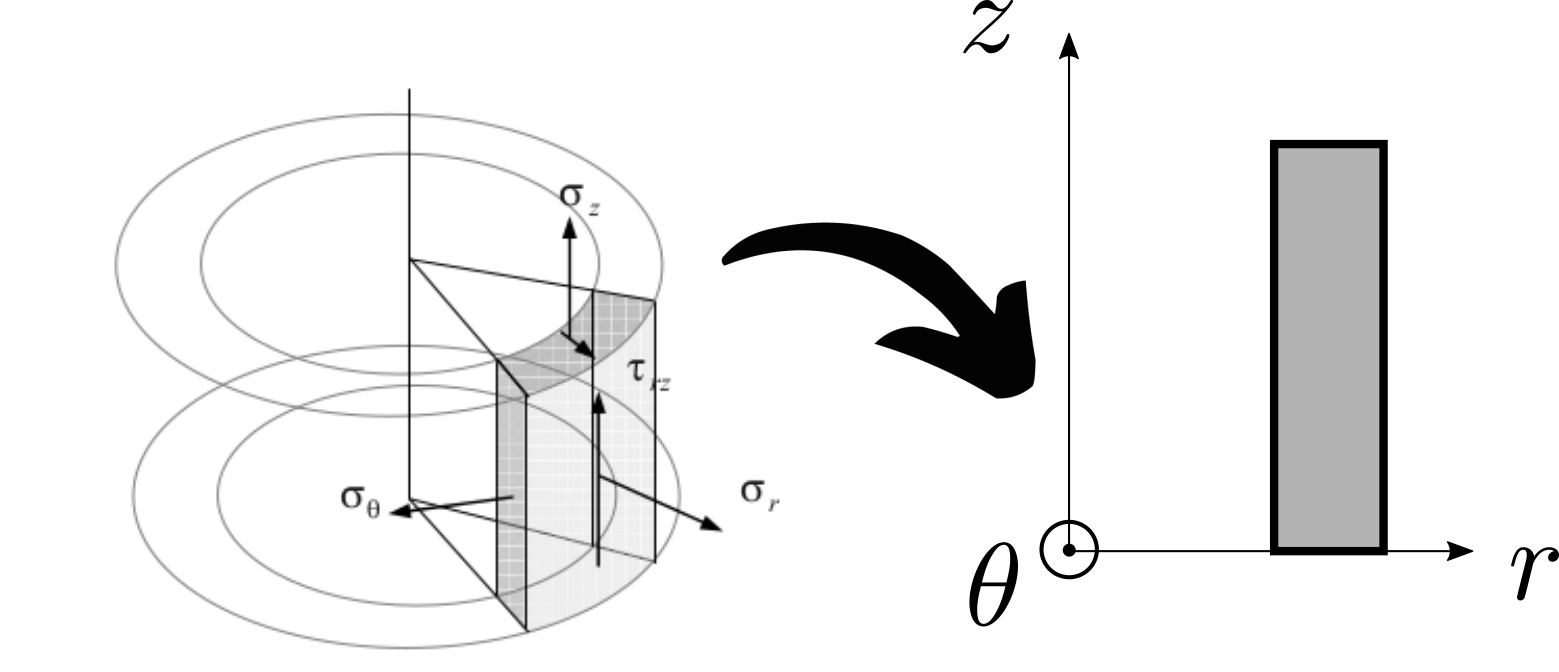
\includegraphics[width=0.7\linewidth]{files/Rotsym-3fba0d8dbcd585e051159d15272d95e0.png}
\caption[]{Rotationssymmetrischer Körper im Zylinderkoordinatensystem $\{r,z,\theta\}$. Nach \cite{chaves2013notes}}
\label{rotsym}
\end{figure}

Die Dehnungen für rotationssymmetrische Problemstellungen werden berechnet zu:

\begin{equation}
\label{rotsymstrain}
\begin{bmatrix}
\e_{r} \\
\e_z \\
\e_{\theta} \\
\gamma_{rz}
\end{bmatrix} = \begin{bmatrix}
\Pd{u}{r} \\
\Pd{v}{z} \\
\frac{u}{r} \\
\Pd{u}{z} + \Pd{v}{r}
\end{bmatrix}
\end{equation}

Das generalisierte Hooke'sche Gesetz lautet:

\begin{equation}
\label{generalHookRotsym}
\begin{bmatrix} 
\sigma_{rr} \\
\sigma_{zz} \\
\sigma_{\theta} \\
\sigma_{rz} \\
\end{bmatrix} = \frac{E}{(1+\nu)(1-2\nu)}\begin{bmatrix}
1-\nu & \nu & \nu & 0  \\
\nu & 1-\nu & \nu & 0  \\
\nu & \nu & 1-\nu & 0  \\
0 & 0 & 0 & \frac{1-2\nu}{2} \\
\end{bmatrix} \begin{bmatrix} \epsilon_{r} \\ \epsilon_{\theta} \\ \epsilon_{z} \\ 2\epsilon_{rz}  \end{bmatrix}
\end{equation}

\begin{framed}
\textbf{Berechnung der Dehnung $\e_{\theta}$}\\
Die Dehnung in Umfangsrichtung kann bestimmt werden als Längenänderung des Umfangs infolge einer radialen Verschiebung $u$:

$\e_{\theta} = \frac{2 \pi (r+u) -2\pi r}{2\pi r} = \frac{u}{r}$
\end{framed}

\paragraph{Zusammenfassung}

Um ein valides mechanisches Modell zu erlangen, benötigt man:

\begin{enumerate}
\item Die beschreibende partielle Differentialgleichung (physikalische Erhaltungssätze)
\item Die kinematischen Beziehungen (Verbindung von primärer Grö$\beta$e zur abgeleiteten Grö$\beta$e)
\item Materialmodell (Verbindung von sekundärer Grö$\beta$e zur kinematischen Grö$\beta$e)
\end{enumerate}

Eindeutig lösbar wird das Modell zudem erst, wenn die Randbedingungen entsprechend vorgegeben sind.

\begin{framed}
\textbf{Fragen zum Kapitel}\\
\textbf{Feldgleichungen der Kontinuumsmechanik}

\begin{itemize}
\item Nennen Sie die für die Strukturmechanik wesentliche Feldgleichung.


\item Nennen Sie drei verschiedene Feldgleichungen.


\item Welche Feldgrö$\beta$e wird mit der Impulsbilanz berechnet?


\item Welche Feldgrö$\beta$e wird mit der Energiebilanz berechnet?


\item Welche Feldgrö$\beta$e wird mit der Massenbilanz berechnet?


\item Was ist der Unterschied zwischen primären und sekundären Feldgrö$\beta$en?


\item Welche Aussage ist richtig:

\begin{itemize}
\item Die Impulsbilanz ist eine vektorielle partielle Differenzialgleichung.
\item Die Energiebilanz ist eine vektorielle partielle Differenzialgleichung.
\item Die sekundäre Feldgrö$\beta$e der Energiebilanz ist der Wärmefluss.
\item Die Massenbilanz ist für gewöhnliche Festkörper stets erfüllt und muss nicht separat gelöst werden.
\item Die Bilanzgleichungen sind materialunabhängige physikalische Prinzipien.
\item Zur Lösung der Bilanzgleichungen benötigt man noch weitere Restriktionen.
\end{itemize}


\item Welche Arten von Randbedingungen werden in der Mechanik von Festkörpern unterschieden?


\item Ist eine Kraftrandbedingung eine \textit{Neumann}-Randbedingung oder eine \textit{Dirichlet}-Randbedingung?


\item Ist eine Verschiebungsrandbedingung eine \textit{Neumann}-Randbedingung oder eine \textit{Dirichlet}-Randbedingung?
\end{itemize}

%  -+-+-+-+-+-+-AI-SPLIT

\textbf{Kinematik}

\begin{itemize}
\item Welche Aussage ist richtig:\begin{itemize}
\item Die Dehnung ist der symmetrische Anteil des Verschiebungsgradienten.
\item Die Spannung ist der symmetrische Anteil des Verschiebungsgradienten.
\item Die Ingenieursdehnungen sollten nur in einem Dehnungsbereich von \textless  10 \% eingesetzt werden.
\item Starrkörperrotationen rufen keine Ingenieurdehnungen (und auch keine Spannungen) hervor.
\end{itemize}
\end{itemize}

\textbf{Materialgleichung}

\begin{itemize}
\item Warum brauchen wir Materialgleichungen? (2 Gründe nennen)
\item Nennen Sie eine Klasse von Materialien entsprechend ihres Materialverhaltens für strukturmechanische Problemstellungen.
\item In welche Richtung flie$\beta$t die Temperatur bei der Fourierschen Wärmeleitung?
\item Was bedeutet isotropes Materialverhalten?
\item Wie viele Materialparameter sind nötig, um das Verhalten von linearen, isotropen und elastischen Materialien zu beschreiben?
\item Liegt bei Karosserieteilen eher ein ebener Spannungs- oder ein ebener Verzerrungszustand vor?
\end{itemize}

\textbf{Zusammenfassung}

\begin{itemize}
\item Welche 3 Dinge sind erforderlich, um ein lösbares mechanisches Modell zu erhalten?
\item Was ist zusätzlich notwendig, um eine eindeutige Lösung zu erhalten?
\end{itemize}

%  -+-+-+-+-+-+-AI-SPLIT
\end{framed}

\subsubsection{Grundgleichungen einfacher Strukturelemente}

\begin{figure}[!htbp]
\centering
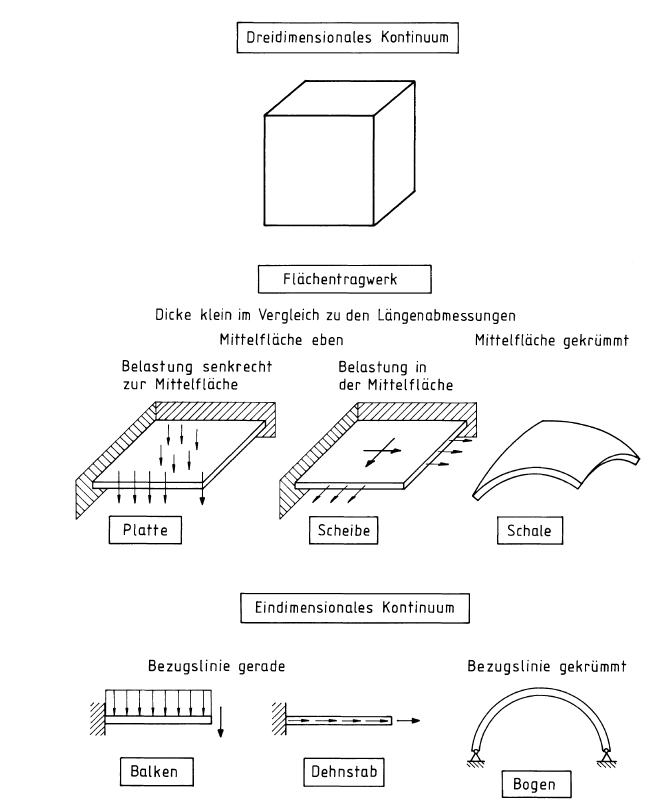
\includegraphics[width=0.75\linewidth]{files/Strukturelemente_Kno-8d4021870da8e52347739e58730bf650.png}
\caption[]{Übersicht über die Klassifizierung von Strukturvereinfachungen nach \cite{knothe1991finite}}
\label{strukturkontinua}
\end{figure}

Die im vorherigen Abschnitt eingeführten Feldgleichungen lassen sich für viele ingenieurwissenschaftliche Problemstellungen deutlich vereinfachen. In Figure~\ref{strukturkontinua} sind solche Vereinfachungen dargestellt.

Für die Impulsbilanz haben wir bereits in der Vorlesung zur ``Technischen Mechanik 2'' zwei Vereinfachungen kennengelernt:

\begin{itemize}
\item den Dehnstab
\item den Balken
\end{itemize}

Nachfolgend werden lediglich die Differentialgleichungen dieser beiden Strukturelemente eingeführt. Für eine Herleitung der Gleichungen sei auf die entsprechende Vorlesung verwiesen.

\paragraph{Differentialgleichung des Stabes}

Wird ein prismatisches Bauteil nur entlang seiner Achse $x$ belastet, so resultieren hieraus nur Normalspannungen $\sigma_x$. Solche Belastungsszenarien können über die Differentialgleichung des \textbf{Stabes} in guter Näherung beschrieben werden.

\begin{figure}[!htbp]
\centering
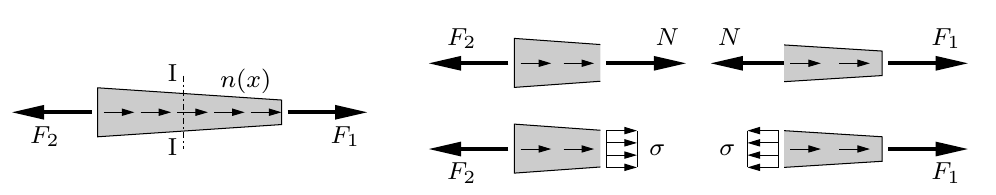
\includegraphics[width=0.75\linewidth]{files/Stab_TMKompakt-28bf6db8104e11c4fddde1fa0352bfd3.png}
\caption[]{Kräftegleichgewicht und Spannungen am geraden Stab nach \cite{wriggers2006technische}}
\label{stab}
\end{figure}

Die Differentialgleichung des Stabes lautet:

\begin{equation}
\label{stabdgl}
\frac{\text{d } \left( E(x)A(x) \frac{\text{d } u}{\text{d } x} \right) }{\text{d } x} =  \frac{\text{d } \left(E(x)A(x) \alpha_T(x) \Delta \theta\right)}{\text{d } x} - n(x)
\end{equation}
mit:

\begin{itemize}
\item $E$ - Elastizitätsmodul in MPa
\item $A$ - Querschnittsfläche in mm\textsuperscript{2}
\item $u$ - axiale Verschiebung in mm
\item $\alpha$ - Wärmeausdehnungskoeffizient in mm/K
\item $\Delta \theta$ - Temperaturänderung in K
\item $n$ - axiale Streckenlast in N/mm
\end{itemize}

Für einen konstanten $E$-Modul, eine konstante Querschnittsfläche $A$ sowie eine konstante Temperaturdifferenz $\Delta \theta$ kann diese Differentialgleichung vereinfacht werden zu:

\begin{equation}
\label{stabdglsimple}
 u^{\prime \prime} = \frac{\text{d}^2\,  u  }{\text{d } x^2} =  - \frac{n(x)}{EA}
\end{equation}

%  -+-+-+-+-+-+-AI-SPLIT

\paragraph{Differentialgleichung des Balkens}

Balken sind Tragstrukturen, die eindimensional modelliert werden, da ihre Breite und Höhe im Verhältnis zu ihrer Länge sehr gering sind. Im Unterschied zu Stäben, bei denen die Belastung nur in Längsrichtung erfolgt, werden Balken zusätzlich senkrecht zur Längsachse belastet. Dies führt dazu, dass in Stäben ausschlie$\beta$lich Normalkräfte auftreten, während sich in Balken Momente und Querkräfte als Schnittgrö$\beta$en ergeben.

\begin{figure}[!htbp]
\centering
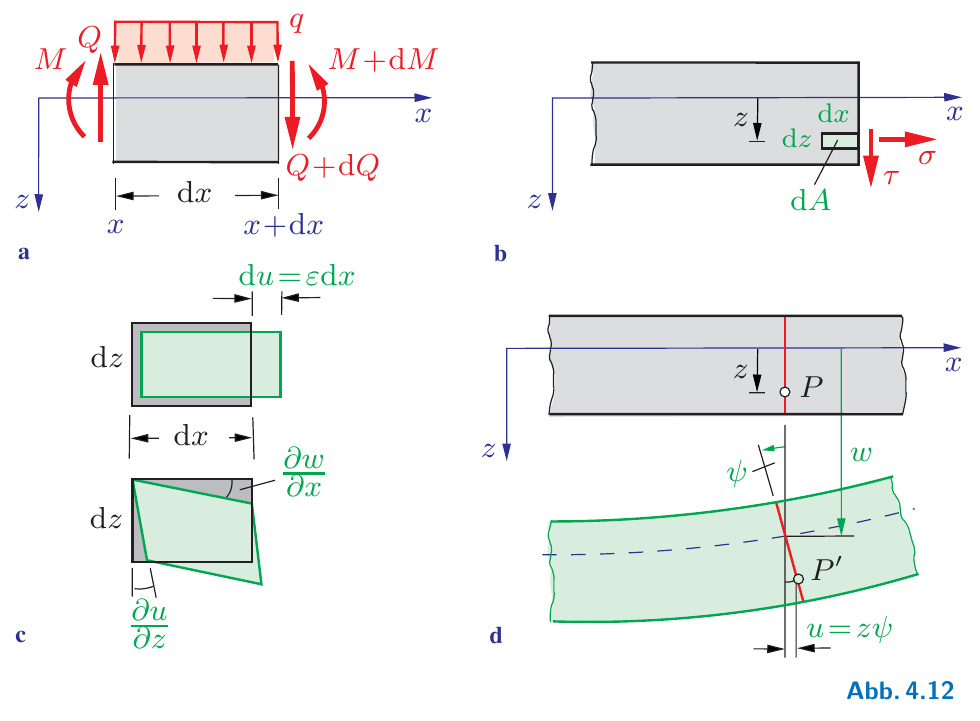
\includegraphics[width=0.75\linewidth]{files/Balken_TM2-bee88dc67566652ab2198dcf3f86b627.png}
\caption[]{Kräftegleichgewicht, Spannungen und Schnittgrö$\beta$en am geraden Balken nach \cite{gross2007technische}}
\label{balken}
\end{figure}

Die Differentialgleichung des Balkens lautet:

\begin{equation}
\label{balkendgl}
 \left(E I_y w^{\prime \prime}\right)^{\prime\prime} =  q(x)
\end{equation}
Für eine konstante Biegesteifigkeit $EI$ vereinfacht sich diese zu:
\begin{equation}
\label{balkendglsimple}
  w^{IV} =  \frac{q(x)}{E I_y}
\end{equation}

\section{Theorie der Finiten Elemente Methode}

\subsection{Die Finite-Elemente-Methode}

In den nachfolgenden Abschnitten werden die Grundzüge der Finite-Elemente-Methode eingeführt. Bei dieser Einführung handelt es sich um eine ingenieurwissenschaftliche Darstellung. Auf mathematische Anforderungen und Restriktionen wird nur bei Bedarf eingegangen. Für eine mathematisch rigorose Herleitung sei an dieser Stelle auf das Buch von Braess \cite{braess2013finite} verwiesen.

%  $
% \newcommand{\MtdFull}[1]{\frac{D \, #1}{D \, t}}
% \newcommand{\Pd}[2]{\frac{\partial #1}{\partial #2}}
% \newcommand{\d}{\text{d} }
% \newcommand{\Dd}[2]{\frac{\d #1}{\d #2}}
% \newcommand{\dt}[1]{#1 ^{\bullet}}
% \newcommand{\dV}{\; \text{d}V}
% \newcommand{\dA}{\; \text{d}A}
% \newcommand{\dx}{\; \text{ d}x}
% \newcommand{\dy}{\; \text{ d}y}
% \newcommand{\dz}{\; \text{ d}z}
% \newcommand{\dxi}{\; \text{ d}\xi}
% \newcommand{\deta}{\; \text{ d}\eta}
% \newcommand{\dzeta}{\; \text{ d}\zeta}
% \newcommand{\grad}[1]{\text{grad}\left(#1\right)}
% \renewcommand{\div}[1]{\text{div} \left(#1\right)}
% \newcommand{\td}[1]{\dot{#1}}
% \newcommand{\tdd}[1]{\ddot{#1}}
% \newcommand{\T}{\rp{T}}
% \newcommand{\rp}[1]{^{\text{#1}}}
% \newcommand{\rs}[1]{_{\text{#1}}}
% \renewcommand{\bm}[1]{\boldsymbol{#1}}
% \newcommand{\e}{\epsilon}
% \newcommand{\eb}{\bm{\e}}
% \newcommand{\s}{\sigma}
% \newcommand{\sb}{\bm{\sigma}}
% $

\subsubsection{Von der starken zur schwachen Form}

Für die in Kapitel 1 eingeführten Randwertprobleme (Massenbilanz, Impulsbilanz und Energiebilanz) werden in diesem Kapitel die theoretischen Grundlagen der Finite Elemente Methode beschrieben. Für jedes der genannten Probleme ist der Ausgangspunkt die \textbf{starke} Form der beschreibenden partiellen Differentialgleichung. Am Beispiel der Impulsbilanz soll exemplarisch die zugehörige \textbf{schwache} Form hergeleitet werden. Die Begriffe stark und schwach beziehen sich hierbei auf die Stetigkeits- und Differenzierbarkeitsanforderungen der gesuchten Lösung $\bm{u}$. Die starke Form hat somit \textbf{immer} höhere Anforderungen an die Lösung.

\begin{figure}[!htbp]
\centering
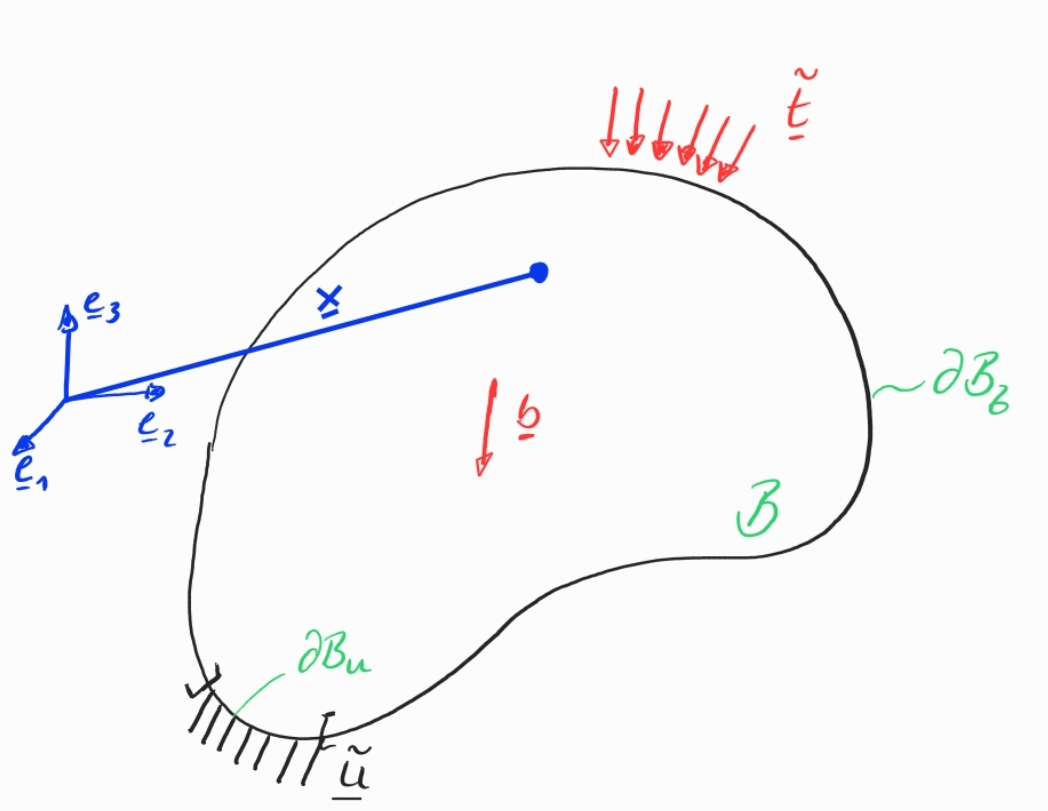
\includegraphics[width=0.7\linewidth]{files/Impulsbilanz-3c1ed32b03eec7db5f7e582ea9b4a7c5.jpg}
\caption[]{Körper $\mathcal{B}$ unter Einwirkung der externen Oberflächenkraft $\tilde{\bm{t}}$ und der Volumenlast $\bm{b}$}
\label{impulsbilanz_fig}
\end{figure}

Ausgangspunkt für die exemplarische Herleitung ist die Impulsbilanz in der quasistatischen Form (ohne Trägheitsterme):

\begin{equation}
\label{weakform_01}
0 = \div{\bm{\sigma}} + \rho \bm{b}
\end{equation}
Diese starke Form wird jetzt mit einer beliebigen vektorwertigen Testfunktion $\delta \bm{u}$ multipliziert und über das betrachtete Gebiet $\mathcal{B}$ (den betrachteten Körper) integriert.

\begin{equation}
\label{weakform_02}
0 = \int_{\mathcal{B}} \delta  \bm{u}\T \left(\div{\bm{\sigma}} + \rho \bm{b} \right) \dV
\end{equation}

Dieser Schritt bedeutet, dass wir im Weiteren versuchen werden, die gekoppelten partiellen Differentialgleichungen nicht punktuell exakt zu erfüllen, sondern im gewichteten integralen Mittel. Für elastomechanische Problemstellungen kann die Testfunktion $\delta \bm{u}$ als virtuelle Verrückung aufgefasst werden, und die Gleichung (\ref{weakform_02}) als das bekannte Prinzip der virtuellen Verrückung angesehen werden. Das hier gezeigte Vorgehen ist jedoch unabhängig von der Elastostatik allgemeingültig.

Als Nächstes integrieren wir die Gleichung (\ref{weakform_02}) partiell. Dafür wenden wir zunächst die Produktregel auf den Divergenzterm an:

\begin{equation}
\label{divergenzsatz}
\int_{\mathcal{B}} \delta \bm{u}\T \div{\bm{\sigma}} \dV = \int_{\mathcal{B}} \div{\delta \bm{u}\T \bm{\sigma}} \dV -\int_{\mathcal{B}} \underbrace{\grad{\delta\bm{u}\T}}_{\delta \bm{\eb}}\bm{\sigma} \dV \; .
\end{equation}

Der Wechsel vom Divergenz-Operator zum Gradienten-Operator im zweiten Term auf der rechten Seite lässt sich schlüssig damit erklären, dass das Resultat ein Skalar sein soll. Während die Divergenz eines Vektors einen Skalar liefert, ergibt der Gradient eines Vektors einen Tensor zweiter Ordnung. Dieser Tensor wird dann in einer doppelten skalaren Multiplikation mit einem weiteren Tensor zweiter Ordnung verknüpft, was letztlich zu einem skalaren Ergebnis führt.

Nun lässt sich mit dem Gau$\beta$'schen Integralsatz der erste Term auf der rechten Seite von Gleichung (\ref{divergenzsatz}) als Integral über den Rand formulieren:

\begin{equation}
\label{gaussIntegralTheorem}
\int_{\mathcal{B}} \div{\delta \bm{u}\T  \bm{\sigma}} \dV = \int_{\partial\mathcal{B}} \delta \bm{u}\T \bm{\sigma}  \bm{n} \dA = \int_{\partial\mathcal{B}} \delta \bm{u}\T \bm{t} \dA \; .
\end{equation}

Dieses Resultat wird jetzt wieder in Gleichung (\ref{weakform_02}) eingesetzt und wir erhalten:

\begin{equation}
\label{weakform_03}
\int_{\mathcal{B}} \delta\eb\T  \bm{\sigma} \dV = \int_{\mathcal{B}} \delta \bm{u}\T \rho \bm{b} \dV + \int_{\partial\mathcal{B}} \delta \bm{u}\T  \bm{t} \dA \; .
\end{equation}

\begin{framed}
\textbf{Was haben wir damit erreicht?}\\
\begin{itemize}
\item Der Oberflächenterm in (\ref{weakform_03}) entspricht den Kraftrandbedingungen
\item Der Term auf der linken Seite in (\ref{weakform_03}) enthält nur noch Ableitungen 1. Ordnung von $\bm{u}$, während in (\ref{weakform_01}) Ableitungen 2. Ordnung gefordert wurden $\rightarrow$ schwächere Anforderungen an $\bm{u}$!
\item Gleichung (\ref{weakform_03}) ist exakt das Prinzip der virtuellen Verrückungen\begin{itemize}
\item Virtuelle Arbeit der Spannungen an den Verzerrungen ist gleich der virtuellen Arbeit der eingeprägten Volumenkräfte plus die virtuelle Arbeit der Oberflächenkräfte
\end{itemize}
\end{itemize}
\end{framed}

Setzen wir jetzt noch als Materialmodell die Beschreibung der linearen Elastizität ein, so erhalten wir final:

\begin{equation}
\label{weakform_04}
\int_{\mathcal{B}} \delta\eb\T \bm{C} \eb \dV = \int_{\mathcal{B}} \delta \bm{u}\T \rho \bm{b} \dV + \int_{\partial\mathcal{B}} \delta \bm{u}\T \cdot \bm{t} \dA \; .
\end{equation}

\begin{framed}
\textbf{Fragen zum Kapitel}\\
\textbf{Finite Elemente Methode}

\begin{itemize}
\item Worauf beziehen sich die Begriffe \textit{starke} und \textit{schwache} Formulierung?
\item Was ist korrekt:\begin{itemize}
\item Bei der schwachen Formulierung wird die Bilanzgleichung nur noch im integralen Mittel gelöst.
\item Das Prinzip der virtuellen Verrückung und die schwache Formulierung der Impulsbilanz sind äquivalent.
\item Die starke Formulierung der Bilanzgleichung enthält Ableitungen höherer Ordnung im Vergleich zur schwachen Formulierung.
\end{itemize}
\end{itemize}
\end{framed}

\subsubsection{Die schwache Form am Beispiel des Stabes}

\begin{figure}[!htbp]
\centering
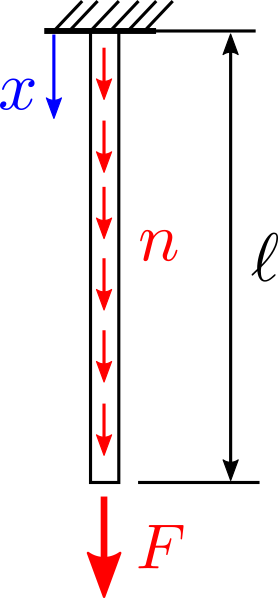
\includegraphics[width=0.25\linewidth]{files/Stab-8a25db6f500d6b4900b1c83a048e0388.png}
\caption[]{Stab unter Eigengewicht und externer Kraft.}
\label{stab_fig}
\end{figure}

Auch hier beginnen wir mit der starken Form der Differentialgleichung:
\begin{equation}
\label{stabdglsimple_2}
 {EA} u^{\prime \prime} =  - {n(x)} A \; ,
\end{equation}

\begin{framed}
\textbf{Analytische Lösung}\\
Die analytische Lösung erhalten wir durch zweifache Integration und Einsetzen der Randbedingungen:
\begin{equation}
u(x) = \left( \frac{F}{EA} + \frac{n \ell}{E}\right)\cdot x - \frac{1}{2} \frac{n}{E} x^2 \; .
\end{equation}
Die Schnittkraft $N$ berechnet sich wie folgt:
\begin{equation}
N(x) = F + n A (\ell-x).
\end{equation}
\end{framed}

Zur Herleitung der Finite-Elemente-Form multiplizieren wir die starke Form mit der Testfunktion $\delta u$ und integrieren die Gleichung über das Gebiet:
\begin{equation}
\label{stabdglsimple_weak}
 \int_{0}^{\ell} \delta u u^{\prime \prime} \dx = \int_{0}^{\ell} - \delta u \frac{n(x)}{EA} \dx\; .
\end{equation}
Der Ausdruck auf der linken Seite wird umgeformt zu:
\begin{equation}
\label{stabdglsimple_product}
 \int_{0}^{\ell} \delta u u^{\prime \prime} \dx = \int_{0}^{\ell} \left(\delta u u^{\prime}\right)^{\prime} - \delta u^{\prime}  u^{\prime}  \dx\; .
\end{equation}

Ersetzen wir nun $\delta u^{\prime}=\delta \e$ und $u^{\prime}=\e$ und setzen die obige Produktregel in Gleichung (\ref{stabdglsimple_weak}), so erhalten wir:
\begin{align}
 \int_{0}^{\ell} \delta \e \cdot E\e \, A \dx & = \left[\delta u \cdot \sigma A \right]_0^{\ell} + \int_0^{\ell} \delta u \cdot n(x) \dx\;  \\
 & = \left[ \delta u(\ell) \cdot F + \delta u(0) \cdot 0\right]+ \int_0^{\ell} \delta u \cdot n(x) \dx\; .
 \end{align}

\paragraph{Das Verfahren von Ritz}

Als Einführung in die Finite-Elemente-Methoden beginnen wir mit dem Verfahren, welches von Walter Ritz (1878 - 1909) eingeführt wurde. Dies fu$\beta$t auf dem Prinzip der virtuellen Arbeit, formuliert als $\delta U - \delta W = 0$, wobei $\delta U$ für die Arbeit der inneren Kräfte und $\delta W$ für die der äu$\beta$eren Kräfte steht. Für einen einfachen Stab ergibt sich die obige schwache Form (\ref{stabdglsimple_weak2}).

Der nächste Schritt ist die Aufstellung einer Näherungslösung $u_h$ für das Verschiebungsfeld $u$, zum Beispiel durch eine quadratische Funktion:

\begin{equation}
u_h(x) = a_0 + a_1 x + a_2 x^2,
\end{equation}

wobei die Koeffizienten $a_i$ durch Minimierung der virtuellen Arbeit ermittelt werden müssen. Diese Parameter müssen gleichzeitig kinematische Verträglichkeit garantieren und somit die geometrischen Randbedingungen einhalten. Aus $u(0) = 0$ ergibt sich dann $a_0 = 0$. Die benötigte Ableitung des Näherungsansatzes lautet daher:

\begin{equation}
\e = u^{\prime} = a_1 + 2a_2 x.
\end{equation}

Die Variationen dieses Ansatzes werden durch Variieren der Koeffizienten gebildet:

\begin{equation}
\delta u(x) = \delta a_1 x + \delta a_2 x^2
\end{equation}

und

\begin{equation}
\delta \e= \delta a_1 + 2 \delta a_2 x.
\end{equation}

Eingesetzt in das Prinzip der virtuellen Arbeit führt es zu:

\begin{equation}
EA \int_0^{\ell} (\delta a_1 + 2 \delta a_2 x) (a_1 +2 a_2 x) \dx = F (a_1 \ell +a_2 \ell^2) + \int_0^{\ell} (\delta a_1 x + \delta a_2 x^2) n A \dx \; .
\end{equation}

Nach Integration und Herausziehen der Variationen resultiert daraus:

\begin{equation}
\delta a_1\left[EA \ell (a_1 + a_2 \ell) - \frac{1}{2} n A \ell^2 - F \ell\right] + \delta a_2 \left[EA\ell^2(a_1 + \frac{4}{3}a_2\ell) - \frac{1}{3}nA\ell^3 - F\ell^2\right] = 0.
\end{equation}

Da die Variationen beliebig sind, müssen die in eckigen Klammern stehenden Terme jeweils null sein. Daraus folgt ein lineares Gleichungssystem zur Bestimmung der Koeffizienten, das gelöst wird als:

\begin{equation}
a_1 = \frac{F}{EA} + \frac{n \ell}{E} \qquad \text{und} \qquad  a_2 = -\frac{n}{2E}.
\end{equation}

Somit erhalten wir als Näherungslösung für diesen Fall:

\begin{equation}
u_h(x) = \left(\frac{F}{EA} + \frac{n \ell}{E}\right)x - \left(\frac{n}{2E}\right)x^2.
\end{equation}

Man kann leicht erkennen, dass mit diesem quadratischen Ansatz die analytische Lösung der Differentialgleichung rekonstruiert werden konnte.

\begin{framed}
\textbf{Problem}\\
Ein Problem beim Ritz'schen Verfahren ist die Wahl der Ansatzfunktion. Diese muss die Randbedingungen erfüllen und die Stetigkeitsanforderungen der schwachen Form. Für komplexere Probleme ist die Wahl der Ansatzfunktion nicht trivial und oft auch nicht möglich.
\end{framed}

%  -+-+-+-+-+-+-AI-SPLIT

\paragraph{Finite Elemente Formulierung für den Stab}

\subparagraph{Diskretisierung der schwachen Form}

\begin{figure}[!htbp]
\centering
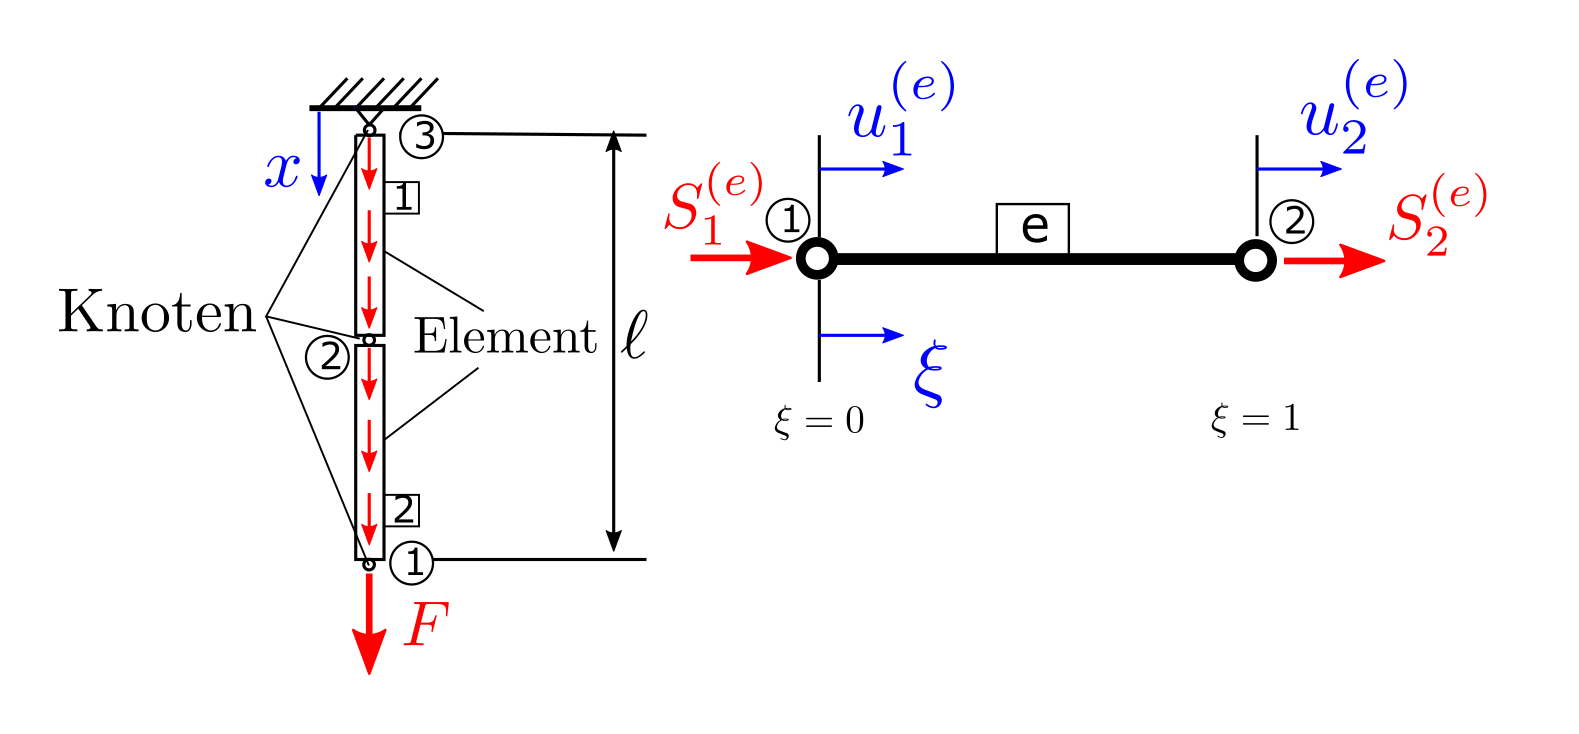
\includegraphics[width=0.75\linewidth]{files/Stab_element-be352cad5b74b55eb9e4829b97d1c026.png}
\caption[]{Stab unter Eigengewicht und externer Kraft mit Stabelementen diskretisiert.}
\label{stabelement}
\end{figure}

Im vorangegangenen Abschnitt haben wir die Effektivität des Prinzips der virtuellen Arbeit in Kombination mit dem Ritz'schen Verfahren untersucht. Es erweist sich jedoch oft als schwierig, einen angemessenen Näherungsansatz für komplexe Strukturen zu finden, die einer vielschichtigen Belastung ausgesetzt sind. Die Finite-Elemente-Methode (FEM) löst dieses Problem, indem sie einfache Ansatzfunktionen auf überschaubaren Teilbereichen -- den sogenannten finiten Elementen -- anwendet und diese dann systematisch für das gesamte Gebiet integriert.

Als Beispiel hierfür dient die im Bild Figure~\ref{stabelement} dargestellte Diskretisierung eines Stabes mit der Gesamtlänge $\ell$, der in zwei finite Elemente mit jeweils der Länge $l_i = \frac{\ell}{2}$ unterteilt wird.

\begin{framed}
\textbf{Allgemeines zu Finiten Elementen}\\
Ein finites Element besteht in dem vorliegenden Beispiel aus 2 Knoten. Sowohl die Knoten als auch die Elemente werden im Allgemeinen nummeriert, damit man sie eindeutig ansprechen kann. Im Bild sind die Elementnummern in den rechteckigen Kästen neben dem Element eingetragen. Die Knotennummern sind in den Kreisen neben den Knoten dargestellt. Die Knoten sind die Träger der primären Feldvariablen (hier: Verschiebung $u$), und das Ziel der Finite-Elemente-Berechnung ist die Bestimmung der primären Variablen, auch Freiheitsgrade (englisch: Degree of freedom \textbf{Dof}) an den Knoten. Im Bild Figure~\ref{stabelement} auf der rechten Seite ist ein einzelnes Stabelement dargestellt. Das Stabelement hat 2 lokale Knoten, und um die Verschiebung an diesen Knoten eindeutig zuzuordnen, verwenden wir die Notation:

$u_1^{e} \text{ Verschiebung } u \text{ am lokalen Knoten 1 von Element } e$

$u_2^{e} \text{ Verschiebung } u \text{ am lokalen Knoten 2 von Element } e$
\end{framed}

Auf diesen Elementen werden dann einfache Ansatzfunktionen verwendet, welche eine lineare Approximation des Verschiebungsfeldes darstellen:

\begin{align}
 N_1(\xi) & = (1-\xi) \qquad N_2(\xi)= \xi  \\
 u_h(\xi) & = N_1(\xi) u_1^{(e)}+ N_2(\xi) u_2^{(e)} \\
 u_h(\xi) & = \sum_{I=1}^2 N_I(\xi) u_I^{(e)}
 \end{align}

Hierbei wurde das lokale Koordinatensystem $\xi = \frac{x}{\ell_e} \; \in \; [0,1]$  eingeführt, damit der gewählte Ansatz für alle Stabelemente, unabhängig von der Stablänge $\ell_e$, gültig ist. In der Matrixschreibweise erhält man für den Ausdruck (\ref{LinearDisplacementAnsatz}):

\begin{align}
  u_h(\xi) & = \underbrace{\begin{bmatrix} (1-\xi) & \xi \end{bmatrix}}_{\bm{N}\T} \underbrace{\begin{bmatrix} u_1^{(e)} \\ u_2^{(e)}\end{bmatrix}}_{\bm{u}^{(e)}} = \bm{N}\T \bm{u}^{(e)}
 \end{align}

Zur Berechnung des Prinzips der virtuellen Verrückungen bzw. der schwachen Form wird zusätzlich die Ableitung des Ansatzes für $u_h$ benötigt. Diese repräsentiert die Dehnung des Stabes $\e = \Dd{u}{x}$. Da der Ansatz über die normalisierte Koordinate $\xi$ bestimmt wurde, berechnet sich die Ableitung über die Kettenregel:

\begin{equation}
\e_h = \Dd{u_h}{x} = \Dd{u_h}{\xi} \underbrace{\Dd{\xi}{x}}_{\frac{1}{\ell_e}} = \frac{1}{\ell_e} \begin{bmatrix} -1 & 1 \end{bmatrix} \begin{bmatrix} u_1^{(e)} \\ u_2^{(e)}\end{bmatrix}
\end{equation}

Für die Variation $\delta u$ und $\delta \e$ wählen wir den gleichen Ansatz:

\begin{equation}
\delta u_h = \begin{bmatrix}  (1-\xi) & \xi \end{bmatrix} \begin{bmatrix} \delta u_1^{(e)} \\ \delta u_2^{(e)}\end{bmatrix} \qquad \delta \e_h = \frac{1}{\ell_e} \begin{bmatrix} -1 & 1 \end{bmatrix} \begin{bmatrix} \delta u_1^{(e)} \\ \delta u_2^{(e)}\end{bmatrix}
\end{equation}

Betrachten wir nun das Prinzip der virtuellen Verrückungen in Gleichung (\ref{stabdglsimple_weak2}):

\begin{align}
 \textcolor{green}{\int_{0}^{\ell} \delta \e \cdot E\e \, A \dx} -\textcolor{red} {\int_0^{\ell} \delta u \cdot n A \dx} - \textcolor{blue}{\delta u(\ell) \cdot F} = 0\; 
 \end{align}

Setzen wir hier unseren gewählten Ansatz für $u$, $\e$, $\delta u$ und $\delta \e$ ein, dann erhalten wir die folgende Gleichung:

\begin{align}
 \textcolor{green}{\int_{0}^{1} \frac{1}{\ell_e} \begin{bmatrix} -1 & 1 \end{bmatrix} \begin{bmatrix} \delta u_1^{(e)} \\ \delta u_2^{(e)}\end{bmatrix}  EA \frac{1}{\ell_e} \begin{bmatrix} -1 & 1 \end{bmatrix} \begin{bmatrix} u_1^{(e)} \\ u_2^{(e)}\end{bmatrix}   \underbrace{\ell_e \d \xi}_{\dx}} \\
 - \textcolor{red}{\int_0^{1} \begin{bmatrix} (1-\xi) & \xi \end{bmatrix} \begin{bmatrix} \delta u_1^{(e)} \\ \delta u_2^{(e)}\end{bmatrix}  n A \ell_e \d \xi} - \textcolor{blue}{\begin{bmatrix} \delta u_1^{(e)} & \delta u_2^{(e)}\end{bmatrix} \begin{bmatrix} S_1^{(e)} \\ S_2^{(e)} \end{bmatrix}}  = 0\; 
\end{align}
%  -+-+-+-+-+-+-AI-SPLIT

Die Variation der Knotenverschiebung $\delta u_I$ und die Knotenverschiebung $u_I$ sind nicht abhängig von $\xi$ und können somit aus dem Integranden herausgezogen werden:

\begin{align}
 \begin{bmatrix} \delta u_1^{(e)} & \delta u_2^{(e)}\end{bmatrix}\left\{ \textcolor{green}{   \int_{0}^{1} EA \frac{1}{\ell_e} \begin{bmatrix} 1 & -1 \\ -1 & 1\end{bmatrix}  \d \xi \begin{bmatrix} u_1^{(e)} \\ u_2^{(e)}\end{bmatrix}} \right .\\
 \left .- \textcolor{red}{n \ell_e A \int_0^{1} \begin{bmatrix} (1-\xi)  \\ \xi \end{bmatrix}   \d \xi} - \textcolor{blue}{ \begin{bmatrix} S_1^{(e)} \\ S_2^{(e)} \end{bmatrix}} \right\}  = 0\; 
\end{align}

Da die Variation beliebig ist, muss die Gleichung für jeden Faktor separat erfüllt sein. Somit erhält man für jedes Element die Gleichung:

\begin{align}
  \textcolor{green}{   \underbrace{\int_{0}^{1} EA \frac{1}{\ell_e} \begin{bmatrix} 1 & -1 \\ -1 & 1\end{bmatrix}  \d \xi}_{\bm{K}^{(e)}} \begin{bmatrix} u_1^{(e)} \\ u_2^{(e)}\end{bmatrix}} 
 - \textcolor{red}{ \underbrace{n \ell_e A \int_0^{1} \begin{bmatrix} (1-\xi) \\ \xi  \end{bmatrix}   \d \xi}_{\bm{F}_V^{(e)}}} - \textcolor{blue}{ \underbrace{\begin{bmatrix} S_1^{(e)} \\ S_2^{(e)} \end{bmatrix}}_{\bm{F}_K^{(e)}}}  & = 0\; \\
 \textcolor{green}{\bm{K}^{(e)} \bm{u}^{(e)}} &=  \textcolor{red}{\bm{F}_V^{(e)}} + \textcolor{blue}{\bm{F}_K^{(e)} } 
\end{align}
Dabei ist $\bm{K}^{(e)}$ die \textbf{Elementsteifigkeitsmatrix}, $\bm{F}_V^{(e)}$ ist der \textbf{Vektor der äquivalenten Knotenkräfte} aus den verteilten Lasten und $\bm{F}_K^{(e)}$ sind die an den Knotenpunkten \textbf{eingeprägten Kräfte}. Für dieses einfache Element können die Integrale in Gleichung (\ref{stabFEM3}) analytisch berechnet werden. Nach der Integration erhält man:

\begin{align}
 \bm{K}^{(e)} & = EA \frac{1}{\ell_e} \begin{bmatrix} 1 & -1 \\ -1 & 1\end{bmatrix} \\
 \bm{F}_V^{(e)} & = n \ell_e A  \begin{bmatrix} \frac{1}{2} \\ \frac{1}{2} \end{bmatrix} 
\end{align}

Damit wurde die Differentialgleichung 2. Ordnung in eine algebraische Gleichung umgeformt. Wir haben jetzt für die zwei Finiten Elemente zwei \textbf{lokale}, lineare Gleichungssysteme. Diese sind jedoch nicht unabhängig voneinander und müssen im nächsten Schritt in ein \textbf{globales} Gleichungssystem assembliert werden.

\subparagraph{Assemblierung der Finiten Elemente}

Das Ziel dieses Abschnitts ist es, die Entwicklung der Gleichungen für das Gesamtsystem aus den Elementsteifigkeitsmatrizen zu beschreiben. Wir werden die Assemblierungoperationen vorstellen, die hierfür verwendet werden. Diese Operationen sind ein fester Bestandteil der Finite-Elemente-Methode (FEM) und kommen selbst bei den komplexesten Problemen zum Einsatz. Daher ist es wesentlich, diese Verfahren zu beherrschen, um die FEM zu erlernen.

Die Elemente in unserem dargestellten Beispiel (Figure~\ref{stabelement}) werden mit den Nummern 1 und 2 bezeichnet, während die Knoten von 1 bis 3 nummeriert sind; weder die Knoten noch die Elemente müssen in einem FEM-Netz in einer bestimmten Reihenfolge nummeriert sein. Wir kommen hierzu nochmal später in der Vorlesung.

Beachten Sie, dass die Kraftgrö$\beta$en der Elemente $S_i^{(e)}$ mit den Indizes 1 und 2 versehen sind. Dies sind die lokalen Knotennummern. Die Knoten des Netzes sind die globalen Knotennummern. Die lokalen Knotennummern eines Stabelements sind immer in der positiven $\xi$-Richtung mit 1, 2 nummeriert. Die globalen Knotennummern hingegen sind willkürlich.

Wir versuchen nun, die lokalen Kräfte $S_i^{(e)}$ für das Element 1 mit den globalen Verschiebungen in Verbindung zu bringen. Betrachten wir zunächst den Knoten 2, welchen sich Element 1 und 2 teilen. Hier gilt für die Verschiebung:
\begin{align}
  u_2^{(1)} = u_1^{(2)} = u_2 \; .
\end{align}

\begin{equation}
\label{stabFEM5}
\begin{align}
\begin{bmatrix}
0 \\
S_2^{(1)}\\
S_1^{(1)}
\end{bmatrix} + \frac{1}{2}n\ell_1 A_1 \begin{bmatrix}
0 \\
1\\
1
\end{bmatrix} = \frac{E_1A_1}{\ell_1}\begin{bmatrix}
0 & 0 & 0\\
0 & 1 & -1\\
0 & -1 & 1
\end{bmatrix} \begin{bmatrix}
u_1 \\
u_2\\
u_3
\end{bmatrix}
\end{align} \; .
\end{equation}

Dazu haben wir lediglich das Elementgleichungssystem (\ref{stabFEM3}) genommen und die lokalen Freiheitsgrade $u_i^{(e)}$ durch ihre zugeordneten globalen Freiheitsgrade $u_i$ gemä$\beta$ den globalen Knotennummern ersetzt. Gleichzeitig haben wir bereits eine zusätzliche Gleichung (1. Zeile) eingeführt. Deren Sinn wird gleich ersichtlich. Das gleiche Vorgehen wenden wir nun auf das Element 2 an:

\begin{equation}
\label{stabFEM6}
\begin{align}
\begin{bmatrix}
S_2^{(2)} \\
S_1^{(2)} \\
0
\end{bmatrix} + \frac{1}{2}n\ell_2 A_2 \begin{bmatrix}
0 \\
1\\
1
\end{bmatrix} = \frac{E_2A_2}{\ell_2}\begin{bmatrix}
1 & -1 & 0\\
-1 & 1 & 0\\
0 & 0 & 0
\end{bmatrix} \begin{bmatrix}
u_1 \\
u_2\\
u_3
\end{bmatrix}
\end{align} \; .
\end{equation}

Nun liegen uns zwei Gleichungssysteme vor, welche sich auf die gleichen Freiheitsgrade beziehen. Durch eine Addition erhalten wir schlie$\beta$lich:

\begin{equation}
\label{stabFEM7}
\begin{align}
\begin{bmatrix}
S_2^{(2)} \\
S_1^{(2)} + S_2^{(1)} \\
S_1^{(1)}
\end{bmatrix} + \frac{1}{4}n\ell A \begin{bmatrix}
1 \\
1+1\\
1
\end{bmatrix} = \frac{EA}{\ell}\begin{bmatrix}
1 & -1 & 0\\
-1 & 2 & -1\\
0 & -1 & 1
\end{bmatrix} \begin{bmatrix}
u_1 \\
u_2\\
u_3
\end{bmatrix}
\end{align} \; .
\end{equation}

Es bleibt noch übrig, die Stabkräfte (innere Kräfte) $S_i$ mit den externen Kräften in Beziehung zu setzen. Für jeden Knoten kann das Kräftegleichgewicht aufgestellt werden:

\begin{equation}
\label{stabFEM8}
\underbrace{\begin{bmatrix}
S_2^{(2)} \\
S_1^{(2)} \\
0
\end{bmatrix}}_{\bm{F}_K^{(2)}} + \underbrace{\begin{bmatrix}
0 \\
S_2^{(1)} \\
S_1^{(1)}
\end{bmatrix}}_{\bm{F}_K^{(1)}} = \underbrace{\begin{bmatrix}
F \\
0 \\
0
\end{bmatrix}}_{\bm{F}\rs{ext}} + \underbrace{\begin{bmatrix}
0 \\
0 \\
R
\end{bmatrix}}_{\bm{R}} \;.
\end{equation}

Somit können wir die inneren Stabkräfte durch die externen Lasten $\bm{F}\rs{ext}$ und Reaktionskräfte $\bm{R}$ ersetzen:

\begin{equation}
\label{stabFEM9}
\begin{align}
\begin{bmatrix}
F \\
0 \\
R
\end{bmatrix} + \frac{1}{4}n\ell A \begin{bmatrix}
1 \\
1+1\\
1
\end{bmatrix} = \frac{2EA}{\ell}\begin{bmatrix}
1 & -1 & 0\\
-1 & 2 & -1\\
0 & -1 & 1
\end{bmatrix} \begin{bmatrix}
u_1 \\
u_2\\
u_3
\end{bmatrix}
\end{align} \; .
\end{equation}

\begin{framed}
\textbf{Direkte Assemblierung}\\
Innerhalb einer FE-Software werden die entsprechenden Matrizen natürlich nicht explizit zunächst auf die Grö$\beta$e der globalen Matrix ``aufgeblasen'', um sie später zu addieren. Über die Zuordnung von lokaler zur globalen Knotennummer kann dies effizient direkt erfolgen.
\end{framed}

%  -+-+-+-+-+-+-AI-SPLIT

\subparagraph{Lösung des Gleichungssystems}

In der vorliegenden Form ist die Systemsteifigkeitsmatrix singulär und daher kann das lineare Gleichungssystem so nicht gelöst werden. Das bedeutet aus physikalischer Sicht, dass das System in der Lage ist, Starrkörperbewegungen durchzuführen. Um dieses Problem zu beheben, müssen die kinematischen Randbedingungen integriert werden. Dies geschieht durch Partitionierung des linearen Gleichungssystems. Dabei ordnen wir die Verschiebungsgrö$\beta$en in bekannte $\bar{\bm{u}}$ und unbekannte $\bm{u}$ Grö$\beta$en:

\begin{equation}
\label{LGSsolve1}
\begin{bmatrix}
\bm{K}_{uu} & \bm{K}_{u\bar{u}} \\
\bm{K}_{\bar{u}u} & \bm{K}_{\bar{u}\bar{u}}
\end{bmatrix}
\begin{bmatrix}
\bm{u} \\
\bar{\bm{u}}
\end{bmatrix} = \begin{bmatrix} \bm{F}\rs{ext} \\ \bm{R} \end{bmatrix} + \bm{F}_v
\end{equation}
Hierbei repräsentiert $\bm{F}\rs{ext}$ die einwirkenden Knotenkräfte und $\bm{R}$ die Reaktionskräfte, die den vorgeschriebenen Verschiebungsgrö$\beta$en zugeordnet sind. Nun lässt sich die erste Zeile nach den unbekannten Verschiebungen auflösen:

\begin{equation}
\label{LGSsolve2}
\begin{bmatrix}
\bm{K}_{uu}
\end{bmatrix}
\begin{bmatrix}
\bm{u}
\end{bmatrix} = \begin{bmatrix} \bm{F}\rs{ext}\end{bmatrix} + \bm{F}_v - \begin{bmatrix}
\bm{K}_{u\bar{u}} 
\end{bmatrix} \begin{bmatrix}
\bar{\bm{u}}
\end{bmatrix}
\end{equation}

Mit der Lösung dieses linearen Gleichungssystems erhält man die unbekannten Knotenverschiebungen. Anschlie$\beta$end können die unbekannten Reaktionskräfte einfach durch Matrizenmultiplikation bestimmt werden:

\begin{equation}
\label{LGSsolve3}
\begin{bmatrix} \bm{R} \end{bmatrix} = 
\begin{bmatrix}
\bm{K}_{\bar{u}u}
\end{bmatrix}
\begin{bmatrix}
\bm{u}
\end{bmatrix} + \begin{bmatrix}
\bm{K}_{\bar{u}\bar{u}} 
\end{bmatrix} \begin{bmatrix}
\bar{\bm{u}}
\end{bmatrix}- \bm{F}_v
\end{equation}

Im vorliegenden Beispiel erhalten wir für das Gleichungssystem (\ref{LGSsolve2}):

\begin{align}
\begin{bmatrix}
F \\
0 \\
\end{bmatrix} + \frac{1}{4}n\ell A \begin{bmatrix}
1 \\
1+1
\end{bmatrix} - \frac{2EA}{\ell}\begin{bmatrix}
 0\\
-1
\end{bmatrix} \begin{bmatrix}
0
\end{bmatrix} & = \frac{2EA}{\ell}\begin{bmatrix}
1 & -1\\
-1 & 2 \\
\end{bmatrix} \begin{bmatrix}
u_1 \\
u_2\\
\end{bmatrix} \\
\begin{bmatrix}
F +\frac{1}{4}n\ell A \\
\frac{1}{2}n\ell A \\
\end{bmatrix} & =
\frac{2EA}{\ell}\begin{bmatrix}
1 & -1\\
-1 & 2 \\
\end{bmatrix} \begin{bmatrix}
u_1 \\
u_2\\
\end{bmatrix} 
\end{align}

mit der Lösung:

\begin{align}
\begin{bmatrix}
u_1 \\
u_2\\
\end{bmatrix} = \begin{bmatrix}
 \frac{F\ell}{EA} + \frac{n \ell^2}{2E}\\
\frac{F\ell}{2EA} + \frac{3 n \ell^2}{8E}
\end{bmatrix} 
\end{align}

Die unbekannte Reaktionskraft am Knoten 3 berechnet sich dann zu:

\begin{align}
R + F_v & = \frac{2EA}{\ell} \begin{bmatrix}
0 & -1 
\end{bmatrix} \begin{bmatrix}
u_1 \\ u_2
\end{bmatrix} + \begin{bmatrix}
1
\end{bmatrix} \begin{bmatrix}
0
\end{bmatrix} \\
&= -\frac{2EA}{\ell} \left(\frac{F\ell}{2EA} + \frac{3 n \ell^2}{8E} \right)- \frac{1}{4}n\ell A= -F - n \ell A 
\end{align}

%  -+-+-+-+-+-+-AI-SPLIT

\subparagraph{Berechnung der Schnittgrö$\beta$en}

Die Schnittgrö$\beta$en $N^{(i)}=\sigma^{(i)} A$ werden in einer Nachlaufrechnung (Postprocessing) mittels des Materialmodells $\sigma^{(i)}=E\e^{(i)}$ bestimmt. Dabei sind die Schnittkräfte:

\begin{align}
N^{(1)} & = 2\frac{EA}{\ell} \begin{bmatrix} -1 & - \end{bmatrix} \begin{bmatrix} u_3 \\ u_2 \end{bmatrix} = F + \frac{3}{4} n A \ell \\
N^{(2)} & = 2\frac{EA}{\ell} \begin{bmatrix} -1 & 1 \end{bmatrix} \begin{bmatrix} u_2 \\ u_1 \end{bmatrix}= F + \frac{1}{4} n A \ell
\end{align}

\subparagraph{Diskussion der Ergebnisse}

Abbildung \ref{FE-compare} links zeigt einen Vergleich zwischen dem mit der Finite-Elemente-Methode (FEM) ermittelten Verschiebungsfeld und der analytischen Lösung. Letztere zeigt aufgrund der Eigengewichtsbelastung einen quadratischen Verlauf, während die FEM diesen in Abschnitten durch lineare Näherungen darstellt. In diesem speziellen Fall ist erkennbar, dass die FEM die analytische Lösung an den Knotenpunkten exakt wiedergibt.

Im rechten Teil von Abbildung \ref{FE-compare} wird die FE-Approximation für den Verlauf der Schnittkräfte mit der analytischen Lösung kontrastiert. Die analytische Lösung zeigt ein lineares Wachstum der Normalkraft auf, das jedoch durch die hier verwendeten linearen Ansatzfunktionen lediglich stückweise durch eine konstante Annäherung wiedergegeben wird. Dabei treten an den Grenzen der Elemente Diskontinuitäten in den von der FEM berechneten Schnittkraftverläufen auf. Auffällig ist auch in diesem Beispiel, dass die analytische Lösung im Zentrum jedes Elements exakt erreicht wird.

Die Genauigkeit dieser Näherungslösung kann augenscheinlich gesteigert werden, indem man die Anzahl der Elemente erhöht. Dies führt dazu, dass die Sprünge im Verlauf der Schnittkräfte bestehen bleiben, aber kleiner ausfallen. Um eine qualitativ signifikante Verbesserung zu erzielen, empfiehlt es sich, Elemente mit quadratischen Ansatzfunktionen für das Verschiebungsfeld zu nutzen. In diesem Fall wird bereits mit einem einzigen Element, das über drei Knotenpunkte verfügt, die exakte Lösung erlangt. In dieser Situation wäre dann die FEM äquivalent dem Ritz'schen Verfahren.

%  -+-+-+-+-+-+-AI-SPLIT

\subparagraph{Konvergenz der Ergebnisse}

\begin{figure}[!htbp]
\centering
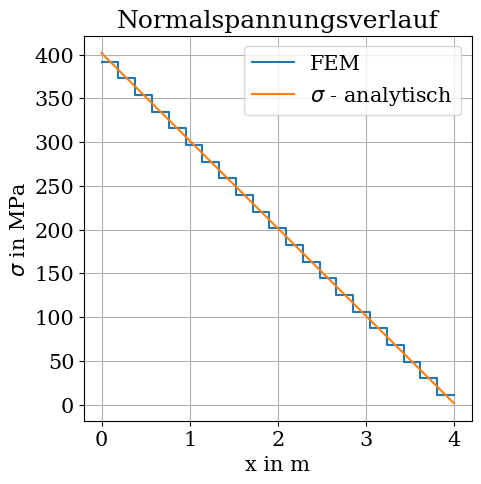
\includegraphics[width=0.75\linewidth]{files/Stab_Normalkraft_ref-092130b8e6ecfe32c195825bcc7079b4.png}
\caption[]{Ergebnisse für die Normalspannung in einem Stab unter Eigengewicht mit einer erhöhten Netzfeinheit.}
\label{stabelement_refined}
\end{figure}

Bei einer immer feiner werdenden Diskretisierung des Stabes konvergiert die Lösung gegen die analytische Lösung. Dennoch liegen, wie in Abbildung Figure~\ref{stabelement_refined} zu sehen, immer noch Spannungssprünge an den Elementgrenzen vor. Betrachtet man die Fehler der Spannungsergebnisse, so zeigt sich, dass dieser Fehler mit steigender Anzahl an Freiheitsgraden abnimmt. Dies ist in Abbildung Figure~\ref{stabelement_error} zu sehen. Im doppelt logarithmischen Ma$\beta$stab erhält man eine Gerade für die Abnahme des Fehlers. Auch bei der Verwendung von Ansatzfunktionen höherer Ordnung reduziert sich der Fehler nur linear im doppelt logarithmischen Ma$\beta$stab. Die Steigung ist jedoch höher, sodass im Allgemeinen mit einer verbesserten Konvergenz zu rechnen ist.

\begin{figure}[!htbp]
\centering
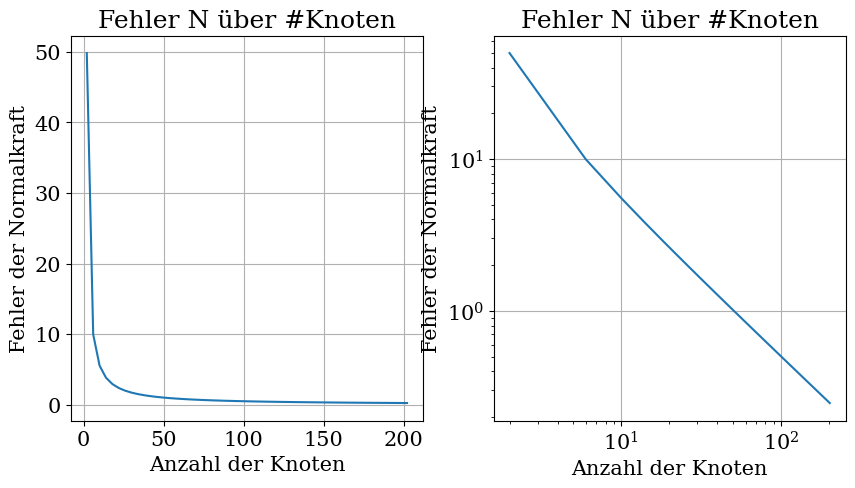
\includegraphics[width=0.75\linewidth]{files/Stab_error_convergen-416e1c43fb4900af48fee79e64009d70.png}
\caption[]{Konvergenz der Spannungsergebnisse in einem Stab unter Eigengewicht mit steigender Anzahl an Freiheitsgraden.}
\label{stabelement_error}
\end{figure}

\paragraph{Interaktives Notebook}

Basierend auf der präsentierten Theorie wurde ein Jupyter Notebook erstellt. Dieses kann man ohne Systemvoraussetzungen im Browser ausführen:

StabFEM for Binder: \href{https://mybinder.org/v2/gh/steffenbeese/FEM\_I\_Notebooks/main?urlpath=\%2Fdoc\%2Ftree\%2FNotebook\_StabFEM.ipynb}{
\includegraphics[width=0.2\linewidth]{files/b77199e99a54e59b2e3c037c2cc90f21.pdf}
}

\begin{framed}
\textbf{Fragen zum Kapitel}\\
\textbf{StabFEM}

\begin{itemize}
\item Was unterscheidet das Verfahren von Ritz von der FEM?
\item Welches Problem hat man beim Verfahren von Ritz bezüglich der Ansatzfunktion?
\item Skizzieren Sie die Formfunktionen für ein lineares Stabelement mit 2 Knoten.
\item Auf Elementebene werden die Steifigkeitsmatrizen und die Lastvektoren berechnet. Was passiert danach mit diesen Grö$\beta$en?
\item Das globale Gleichungssystem kann nicht gelöst werden. Die Steifigkeitsmatrix ist singulär. Was könnte der Grund dafür sein?
\end{itemize}
\end{framed}

%  $
% \newcommand{\MtdFull}[1]{\frac{D \, #1}{D \, t}}
% \newcommand{\Pd}[2]{\frac{\partial #1}{\partial #2}}
% \newcommand{\d}{\text{d} }
% \newcommand{\Dd}[2]{\frac{\d #1}{\d #2}}
% \newcommand{\dt}[1]{#1 ^{\bullet}}
% \newcommand{\dV}{\; \text{d}V}
% \newcommand{\dA}{\; \text{d}A}
% \newcommand{\dx}{\; \text{ d}x}
% \newcommand{\dy}{\; \text{ d}y}
% \newcommand{\dz}{\; \text{ d}z}
% \newcommand{\dxi}{\; \text{ d}\xi}
% \newcommand{\deta}{\; \text{ d}\eta}
% \newcommand{\dzeta}{\; \text{ d}\zeta}
% \newcommand{\grad}[1]{\text{grad}\left(#1\right)}
% \renewcommand{\div}[1]{\text{div} \left(#1\right)}
% \newcommand{\td}[1]{\dot{#1}}
% \newcommand{\tdd}[1]{\ddot{#1}}
% \newcommand{\T}{\rp{T}}
% \newcommand{\rp}[1]{^{\text{#1}}}
% \newcommand{\rs}[1]{_{\text{#1}}}
% \renewcommand{\bm}[1]{\boldsymbol{#1}}
% \newcommand{\e}{\epsilon}
% \newcommand{\eb}{\bm{\e}}
% \newcommand{\s}{\sigma}
% \newcommand{\sb}{\bm{\sigma}}
% $

\subsubsection{Die Balken-FEM}

\begin{figure}[!htbp]
\centering
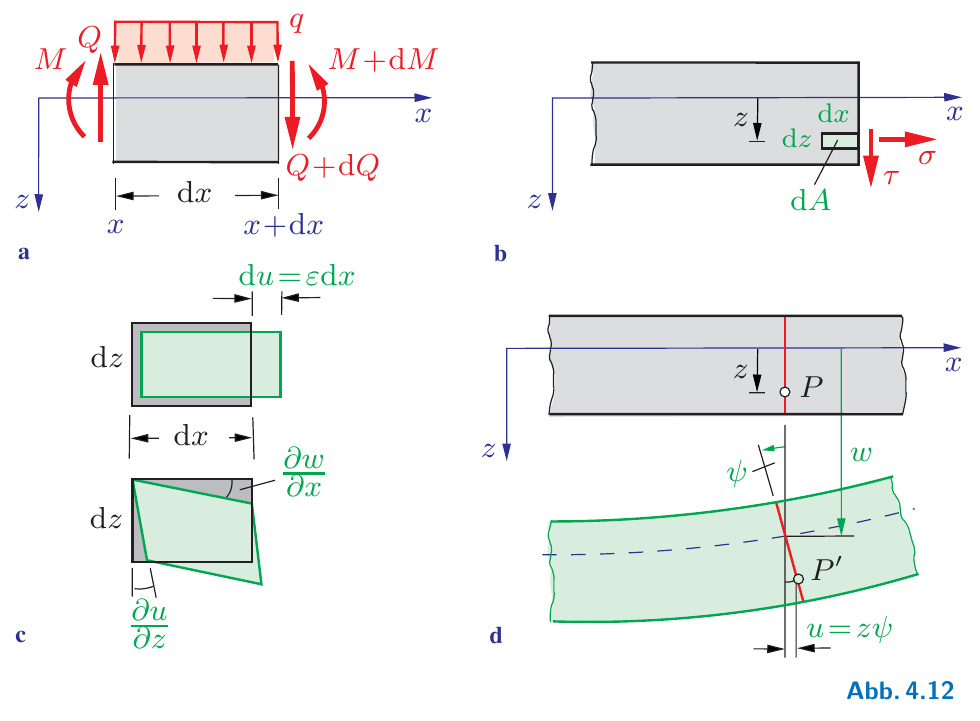
\includegraphics[width=0.7\linewidth]{files/Balken_TM2-047a15c5c31955daed71737e695a57f6.png}
\caption[]{Schnittgrö$\beta$en und Kinematik am Balkenelement nach \cite{gross2007technische}}
\label{balken02}
\end{figure}

Als weiteren Vertreter der Strukturelemente innerhalb der Finite-Elemente-Methode (FEM) betrachten wir im Folgenden die Balken-FEM. Die Impulsbilanz des Euler-Bernoulli-Balkens ist eine Differentialgleichung 4. Ordnung. Unter der Voraussetzung einer konstanten Biegesteifigkeit $EI_y$ lautet diese:

\begin{equation}
\label{balkendglsimple_2}
  w^{IV} =  \frac{q(x)}{E I_y} \; .
\end{equation}
Die obige \textbf{starke Form} der Balken-DGL wird im Folgenden in eine \textbf{schwache Form} umgewandelt. Formal wird die Differentialgleichung wieder mit einer beliebigen Testfunktion $\delta w$ multipliziert und über den Balken integriert. Die schwache Form lautet dann:

\begin{equation}
\label{weakBalken_01}
  EI_y \int_L \delta w'' w'' \dx - \int_L q(x) \delta w \dx - F_I \delta w_I - M_J \delta w'_J = 0 \; .
\end{equation}

Hierbei stellen $F_I$ und $M_I$ die an den Knoten angreifenden Einzellasten und Momente dar. Es ist zu beachten, dass die zweite Ableitung der Durchbiegung die höchste Ableitungsordnung in dieser Variationsgleichung darstellt. Für die Finite-Elemente-Approximation müssen ($C^1$)-stetige Ansatzfunktionen formuliert werden. Dies impliziert, dass an den Knotenpunkten die Verschiebungsansätze sowohl in der Durchbiegung ($w$) als auch in der Neigung ($w'$) stetig sein müssen. Anders als beim Stabelement sind die Freiheitsgrade an den Knotenpunkten nicht nur die Verschiebungen, sondern auch die Neigungen. Dies ist charakteristisch für die Formulierung von Balkenelementen, aber auch für die Formulierung von Plattenelementen und Schalenelementen.

%  -+-+-+-+-+-+-AI-SPLIT

\paragraph{Ansatzfunktionen}

\begin{figure}[!htbp]
\centering
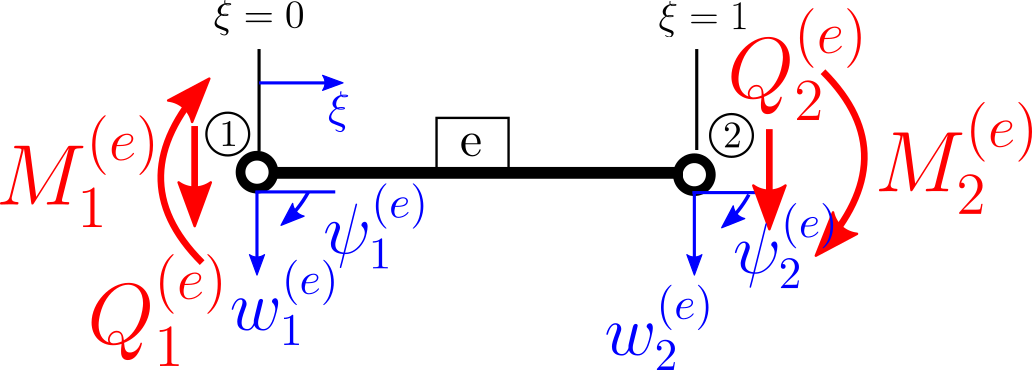
\includegraphics[width=0.7\linewidth]{files/Balkenelement-a8a2414933a947e716e92a521cf26529.png}
\caption[]{Balkenelement mit lokalen Freiheitsgraden}
\label{balken03_1}
\end{figure}

Analog zum Stabelement führen wir die normierte Koordinate $\xi=\frac{x}{\ell_e}$ ein. Die Ansatzfunktionen für die Durchbiegung $w_h$ werden dann als Linearkombination der Formfunktionen $N_I$ und der Freiheitsgrade $w_I$ geschrieben:

\begin{align}
  w_h & = N_1(\xi) w_1 + N_2(\xi) \psi_1 \ell_e +  N_3(\xi) w_2 + N_4(\xi) \psi_2 \ell_e = \sum_{I=1}^{4} N_I(\xi) w_I \\
  & = \begin{pmatrix} N_1(\xi) & N_2(\xi)\ell_e & N_3(\xi) & N_4(\xi)\ell_e \end{pmatrix} \begin{pmatrix} w_1 \\ \psi_1 \\ w_2 \\ \psi_2 \end{pmatrix}
\end{align}

Der Vektor der Freiheitsgrade $\bm{w}=w_I$ enthält die Durchbiegung $w$ und die Neigung $\psi$ an den beiden Knoten des Balkenelements. Wie bei den Formfunktionen des Stabelements ist die Formfunktion $N_I$ nur für den Freiheitsgrad $w_I$ identisch mit 1 und für alle anderen Freiheitsgrade gleich 0. Formfunktionen, die diese Eigenschaft haben, sind zum Beispiel die Hermite-Polynome:
\begin{align}
  \bm{N} = \begin{pmatrix} 
  1-3\xi^2+2\xi^3 \\ 
  (\xi-2\xi^2+\xi^3)\ell_e \\ 
  3\xi^2-2\xi^3 \\ 
  (-\xi^2+\xi^3)\ell_e \end{pmatrix}
\end{align}

%  
% ```{code-cell} ipython3
% ---
% mystnb:
%   figure:
%     caption: Formfunktionen für ein Balkenelelement mit Hermite-Interpolation.
%     name: Shape-Beam
% tags: [
%   "remove-input"
%   ]
% ---
% import numpy as np
% import plotly.graph_objects as go
% 
% # Define the x values
% x = np.linspace(0, 1, 100)
% 
% # Define the shape functions - Hermite polynomials 4th order
% N1 = 1 - 3*x**2 + 2*x**3
% N2 = x - 2*x**2 + x**3
% N3 = 3*x**2 - 2*x**3
% N4 = -x**2 + x**3
% 
% # Create the figure
% fig = go.Figure()
% 
% # Add traces for each shape function
% fig.add_trace(go.Scatter(x=x, y=N1, mode='lines', name='N_1'))
% fig.add_trace(go.Scatter(x=x, y=N2, mode='lines', name='N_2'))
% fig.add_trace(go.Scatter(x=x, y=N3, mode='lines', name='N_3'))
% fig.add_trace(go.Scatter(x=x, y=N4, mode='lines', name='N_4'))
% 
% # Update layout with LaTeX math
% fig.update_layout(
%     xaxis_title=r'$\eta$',
%     yaxis_title=r'$N(\eta)$',
%     legend=dict(x=1.05, y=1),
%     font=dict(family="Serif", size=15),
%     template='plotly_white',
%     xaxis=dict(showgrid=True, gridcolor='grey', gridwidth=0.6, griddash='dash'),
%     yaxis=dict(showgrid=True, gridcolor='grey', gridwidth=0.6, griddash='dash')
% )
% 
% # Show the plot
% # fig.show()
% ```

\begin{framed}
\textbf{Wichtige Eigenschaften des Ansatzes des Balkens}\\
\begin{itemize}
\item Die Durchbiegung $w$ ist $C^1$-stetig.
\item Die Durchbiegung $w$ und die Neigung $\psi=w'$ sind über die Elementgrenzen hinweg stetig.
\item Durch die Wahl der Formfunktionen haben die Knotenfreiheitsgrade die Bedeutung von Durchbiegung und Neigung.
\end{itemize}
\end{framed}

Auch für die Testfunktion $\delta w$ wird der Ansatz (\ref{Ansatz_Balken}) verwendet.

%  -+-+-+-+-+-+-AI-SPLIT

\paragraph{Elementsteifigkeitsmatrix (Diskretisierung Term 1 in Gleichung (\ref{weakBalken_01}) )}

Eingesetzt in die schwache Form liefert der erste Term die Elementsteifigkeitsmatrix. Hierfür müssen zunächst die Ableitungen des Ansatzes bzgl. $x$ berechnet werden. Aus
$\dx = \ell_e \dxi$ folgt:
\begin{align}
  \Dd{w}{x} & = \frac{1}{\ell_e} \Dd{w}{\xi} = \frac{1}{\ell_e} \bm{N}_{,\xi} \bm{w} \\
  \Dd{^2 w}{x^2} & = \frac{1}{\ell_e^2} \Dd{^2 w}{\xi^2} = \frac{1}{\ell_e^2} \bm{N}_{,\xi\xi} \bm{w}
\end{align}

Eingesetzt in die schwache Form ergibt sich für die Elementsteifigkeit:

\begin{align}
  & \delta \bm{w}^T \frac{EI}{\ell^3_e} \int_0^{1}  \bm{N}_{,\xi\xi}^T \bm{N}_{,\xi\xi} \dxi\, \bm{w} \\
  &= \delta \bm{w}^T \frac{EI}{\ell^3_e} \int_0^{1} \begin{pmatrix}
    12\xi -6 & (6\xi-4)\ell_e  & -12\xi+6 & (6\xi-2)\ell_e 
  \end{pmatrix} \begin{pmatrix}
    12\xi -6 \\
    (6\xi-4)\ell_e  \\
    -12\xi+6 \\
    (6\xi-2)\ell_e 
  \end{pmatrix} \dxi\, \bm{w} \\
  &= \delta \bm{w}^T \frac{EI}{\ell^3_e} \int_0^{1} \begin{pmatrix}\left(12 \xi - 6\right)^{2} & \ell_e \left(6 \xi - 4\right) \left(12 \xi - 6\right) & \left(6 - 12 \xi\right) \left(12 \xi - 6\right) & \ell_e \left(6 \xi - 2\right) \left(12 \xi - 6\right)\\\ell_e \left(6 \xi - 4\right) \left(12 \xi - 6\right) & \ell_e^{2} \left(6 \xi - 4\right)^{2} & \ell_e \left(6 - 12 \xi\right) \left(6 \xi - 4\right) & \ell_e^{2} \left(6 \xi - 4\right) \left(6 \xi - 2\right)\\\left(6 - 12 \xi\right) \left(12 \xi - 6\right) & \ell_e \left(6 - 12 \xi\right) \left(6 \xi - 4\right) & \left(6 - 12 \xi\right)^{2} & \ell_e \left(6 - 12 \xi\right) \left(6 \xi - 2\right)\\\ell_e \left(6 \xi - 2\right) \left(12 \xi - 6\right) & \ell_e^{2} \left(6 \xi - 4\right) \left(6 \xi - 2\right) & \ell_e \left(6 - 12 \xi\right) \left(6 \xi - 2\right) & \ell_e^{2} \left(6 \xi - 2\right)^{2}\end{pmatrix} \dxi\, \bm{w} \\
  &= \delta \bm{w} \underbrace{\frac{EI}{\ell^3} \begin{pmatrix}12 & 6 \ell_e & -12 & 6 \ell_e\\6 \ell_e & 4 \ell_e^{2} & - 6 \ell_e & 2 \ell_e^{2}\\-12 & - 6 \ell_e & 12 & - 6 \ell_e\\6 \ell_e & 2 \ell_e^{2} & - 6 \ell_e & 4 \ell_e^{2}\end{pmatrix}}_{\bm{K_e}} \,  \bm{w}
\end{align}

\paragraph{Diskretisierung der Streckenlast}

Die Streckenlast $q(x)$ hat im Element $e$ im Allgemeinen einen beliebigen Verlauf. Um die Streckenlast zu diskretisieren, wird angenommen, dass die Streckenlast im Element linear veränderlich ist. Es wird also der folgende Ansatz gemacht:

\begin{align}
  q_h(\xi) & = (1-\xi) q_1 + \xi q_2 \\
  & = \sum_I N_I(\xi)  q_I
\end{align}

Wird dieser Ansatz in die schwache Form eingesetzt, so ergibt sich:

\begin{align}
  & \int_L \delta \bm{w}  q(x) \dx \\
  & = \ell \int_{0}^1  \delta \bm{w}(\xi) q_h(\xi)  \dxi \\
  & \delta \bm{w} \ell \int_{0}^1 \begin{pmatrix} 2 \xi^{3} - 3 \xi^{2} + 1\\\ell \left(\xi^{3} - 2 \xi^{2} + \xi\right)\\- 2 \xi^{3} + 3 \xi^{2}\\\ell \left(\xi^{3} - \xi^{2}\right)\end{pmatrix} \begin{pmatrix} q_1 & q_2  \end{pmatrix} \dxi \\
  & = \delta \bm{w} \ell \int_{0}^1 \begin{pmatrix}
  \left(q_{1} \left(1 - \xi\right) + q_{2} \xi\right) \left(2 \xi^{3} - 3 \xi^{2} + 1\right)\\\ell \left(q_{1} \left(1 - \xi\right) + q_{2} \xi\right) \left(\xi^{3} - 2 \xi^{2} + \xi\right)\\\left(- 2 \xi^{3} + 3 \xi^{2}\right) \left(q_{1} \left(1 - \xi\right) + q_{2} \xi\right)\\\ell \left(\xi^{3} - \xi^{2}\right) \left(q_{1} \left(1 - \xi\right) + q_{2} \xi\right)
  \end{pmatrix} \\
  & = \delta \bm{w} \underbrace{ \ell \begin{pmatrix}
  \frac{7 q_{1}}{20} + \frac{3 q_{2}}{20}\\\frac{\ell q_{1}}{20} + \frac{\ell q_{2}}{30}\\\frac{3 q_{1}}{20} + \frac{7 q_{2}}{20}\\- \frac{\ell q_{1}}{30} - \frac{\ell q_{2}}{20}
  \end{pmatrix}}_{\bm{F}_Q}
\end{align}

%  -+-+-+-+-+-+-AI-SPLIT

\paragraph{Beispiel der Balken FEM}

\begin{figure}[!htbp]
\centering
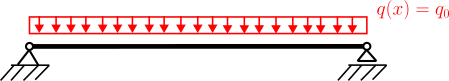
\includegraphics[width=0.7\linewidth]{files/Balken_Problem-ac2d1f8be068071b7e73a411e356e68c.png}
\caption[]{Statisch bestimmt gelagerter Balken mit konstanter Streckenlast}
\label{balken03}
\end{figure}

Für das dargestellte Beispiel eines statisch bestimmten Balkens mit konstanter Streckenlast lässt sich die Lösung der Verschiebung durch vierfache Integration der Differentialgleichung (\ref{balkendglsimple_2}) bestimmen. Die Lösung lautet:

\begin{equation}
\label{Balken_example_01}
EI w(x) =\frac{\ell^{3} q_{0} x}{24} - \frac{\ell q_{0} x^{3}}{12} + \frac{q_{0} x^{4}}{24}
\end{equation}

Über die Beziehungen:

\begin{align}
EI w'' & =-M(x) =  \frac{q_{0} x \left(\ell - x\right)}{2} \\
EI w'''' &= -Q(x) = q_{0} \left(\frac{\ell}{2} - x\right)
\end{align}
erhält man die Schnittgrö$\beta$en für das Biegemoment und die Querkraft.

Wir lösen nun dieses Problem mit der obigen Balken-FEM und vergleichen die Ergebnisse für die Durchbiegung und die Schnittgrö$\beta$en mit der analytischen Lösung.

\begin{figure}[!htbp]
\centering
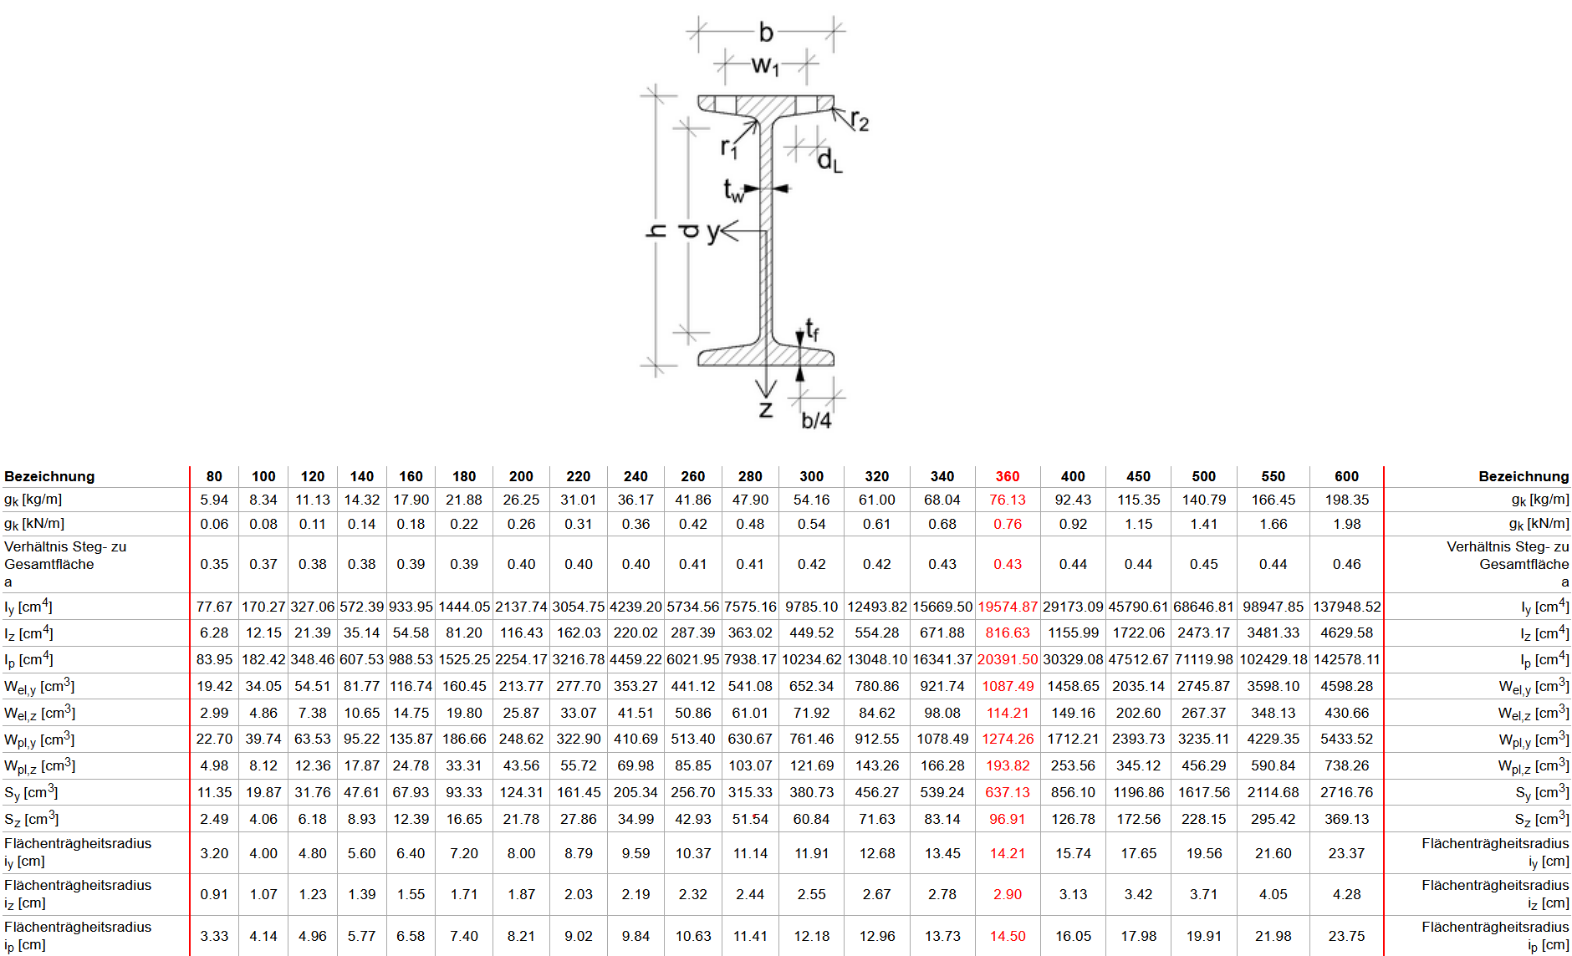
\includegraphics[width=0.8\linewidth]{files/Flächenträgheitsmome-3de341a2d042404c7134255287b1fae2.png}
\caption[]{Flächenträgheitsmomente für I-Profile nach DIN 1025-1:2009-04. \href{https://www.ezzat.org/de/Querschnittswerte/gewalzt/I/i.php}{ezzart.org}}
\label{FT}
\end{figure}

\paragraph{Ergebnisse der FEM-Berechnung}

\begin{figure}[!htbp]
\centering
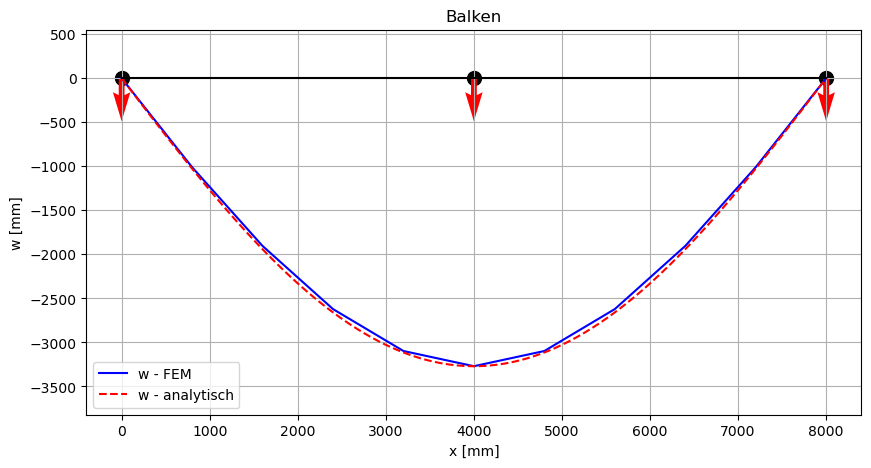
\includegraphics[width=0.625\linewidth]{files/Balken_FEM_01-a1f6ce8daf9026ef9f3fc80e01b3abcb.png}
\caption[]{Gegenüberstellung der analytischen Verschiebungslösung mit der FEM-Lösung.}
\label{BalkenFEM01}
\end{figure}

In Abbildung Figure~\ref{BalkenFEM01} ist die Verschiebungslösung der FEM mit der analytischen Lösung gegenübergestellt. Wir sehen, dass die FEM bereits mit nur 2 Elementen die analytische Lösung exakt trifft. Dies ist kein Zufall, sondern ein Ergebnis der Wahl der Formfunktionen und der Form der Randbedingungen.

Dies sollte jedoch nicht darüber hinwegtäuschen, dass die FEM-Lösung für das Schnittmoment und die Querkraft im Vergleich zur analytischen Lösung nicht so gut ist.

\begin{figure}[!htbp]
\centering
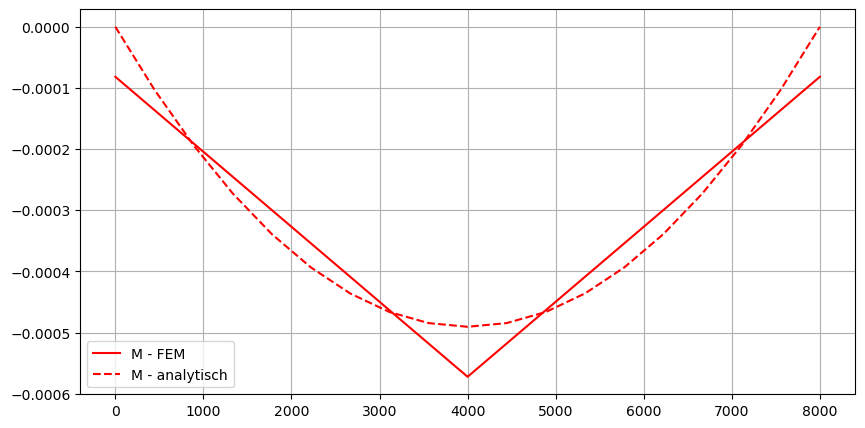
\includegraphics[width=0.625\linewidth]{files/Balken_FEM_02-4862ecf143a8bc5453774a7c198d23b3.png}
\caption[]{Gegenüberstellung der analytischen Lösung des Momentenverlaufs mit der FEM-Lösung.}
\label{BalkenFEM02}
\end{figure}

Das analytische Schnittmoment hat einen quadratischen Verlauf, während die FEM-Lösung linear ist. Dies führt zu einer Abweichung der FEM-Lösung von der analytischen Lösung.

\begin{figure}[!htbp]
\centering
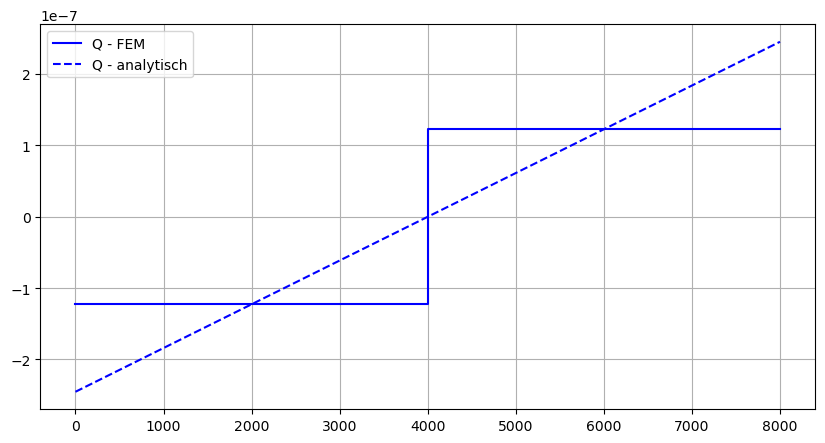
\includegraphics[width=0.625\linewidth]{files/Balken_FEM_03-c04f469fedcb8e67d9db06d983fbd4fd.png}
\caption[]{Gegenüberstellung der analytischen Lösung für den Querkraftverlauf mit der FEM-Lösung.}
\label{BalkenFEM03}
\end{figure}

Die Schnittkraft in der analytischen Lösung zeigt einen stückweise linearen Verlauf, während die FEM-Lösung konstant ist. Dies führt zu einer Abweichung der FEM-Lösung von der analytischen Lösung.

%  -+-+-+-+-+-+-AI-SPLIT

\paragraph{Konvergenz}

\begin{figure}[!htbp]
\centering
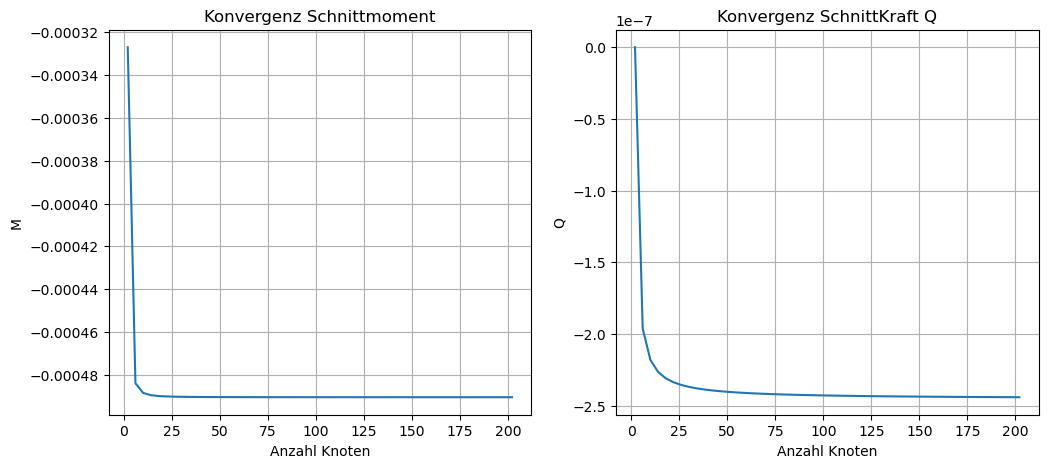
\includegraphics[width=0.75\linewidth]{files/Balken_FEM_04-5989c7a1d613e0755b5bf283d8b43fee.png}
\caption[]{Konvergenzverhalten der FEM-Lösung für das Schnittmoment und die Querkraft.}
\label{BalkenFEM04}
\end{figure}

Allgemein zeigt sich, dass die FEM-Lösung mit zunehmender Anzahl an Elementen gegen die analytische Lösung konvergiert. Dabei ist festzuhalten, dass die Konvergenz des Schnittmoments schneller ist als die Konvergenz der Querkraft. Dies zeigt sich auch im doppelt logarithmischen Diagramm Figure~\ref{BalkenFEM05}. Beide Kurven zeigen eine lineare Abhängigkeit, jedoch ist die Steigung der Konvergenzkurve für das Schnittmoment grö$\beta$er als die Steigung der Konvergenzkurve für die Querkraft.

\begin{figure}[!htbp]
\centering
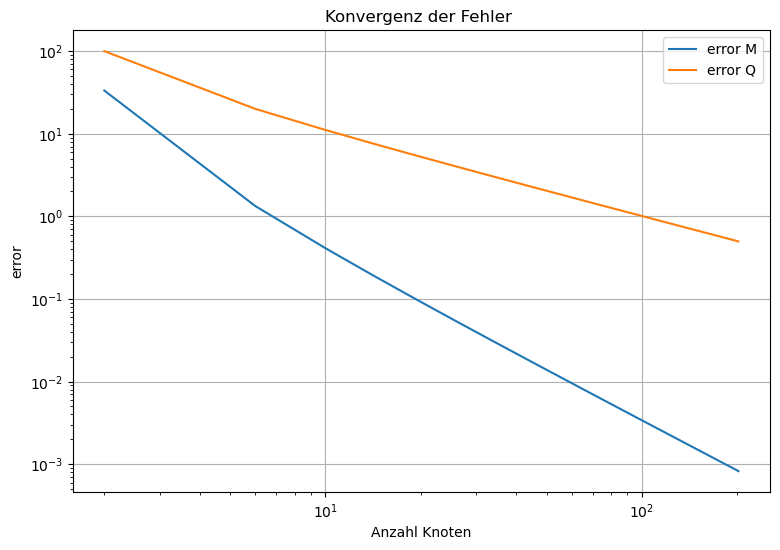
\includegraphics[width=0.75\linewidth]{files/Balken_FEM_05-696ae86f3f41368fe7073b08fecfddd0.png}
\caption[]{Konvergenzverhalten der FEM-Lösung für das Schnittmoment und die Querkraft im doppelt logarithmischen Diagramm.}
\label{BalkenFEM05}
\end{figure}

\paragraph{Interaktives Notebook}

Basierend auf der präsentierten Theorie wurde ein Jupyter Notebook erstellt. Dieses kann man ohne Systemvoraussetzungen im Browser ausführen:

Balken FEM for Binder \href{https://mybinder.org/v2/gh/steffenbeese/FEM\_I\_Notebooks/main?urlpath=\%2Fdoc\%2Ftree\%2FNotebook\_BalkenFEM.ipynb}{
\includegraphics[width=0.2\linewidth]{files/b77199e99a54e59b2e3c037c2cc90f21.pdf}
}

\begin{framed}
\textbf{Fragen zum Kapitel}\\
\textbf{Balken FEM}

\begin{itemize}
\item Welche physikalische Interpretation haben die Knotenfreiheitsgrade beim Balkenelement?


\item Wie gut ist die Lösung der Balken-FEM bzgl. der Verschiebungen im Vergleich zur analytischen Lösung?


\item Welche Aussage ist richtig:

\begin{itemize}
\item Das Schnittmoment ist linear im Element.
\item Die Schnittkraft ist linear im Element.
\item Die Verschiebung ist über die Elementgrenzen stetig.
\item Die Ableitung der Verschiebung ist über die Elementgrenzen stetig.
\end{itemize}
\end{itemize}
\end{framed}

\section{Isoparametrische FEM}

\subsection{Isoparametrische FEM}

\begin{figure}[!htbp]
\centering
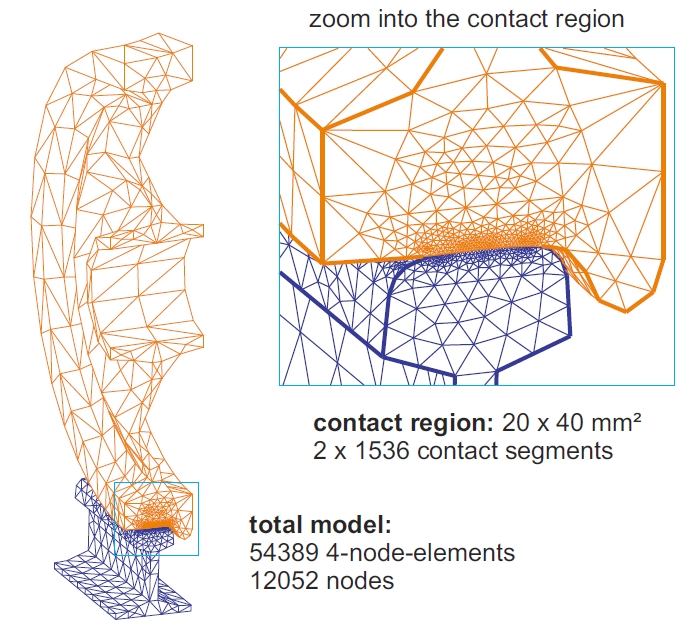
\includegraphics[width=0.75\linewidth]{files/Nackenhorst_01-22e296fb8b98cb3e9d386b83d0613561.png}
\caption[]{Geometrieapproximation am Beispiel der Diskretisierung eines Eisenbahnrades \cite{numerische_mechanik_2022}.}
\label{isogeom}
\end{figure}

Die isoparametrische Finite-Elemente-Methode ist heute der gängige Standard in FEA-Software. Erstmals erwähnt wurde die isoparametrische Finite-Elemente-Methode von I.C. Taig (britischer Luftfahrtingenieur) im Jahre 1958. Die Methode bildet die Grundlage, um komplizierte Geometrien mit gekrümmten Rändern zu modellieren. Als Beispiel sei hier die Diskretisierung in Abbildung Figure~\ref{isogeom} eines Eisenbahnrades gezeigt. In den nächsten Abschnitten werden einige Aspekte der isoparametrischen Finite-Elemente-Methode erläutert. Für einen umfassenderen Einblick sei auf die Standardwerke von \cite{zienkiewicz2005finite}, \cite{hughes2003finite} oder \cite{bathe2006finite} verwiesen.

\subsubsection{Begriffsklärung}

In der schwachen Form (\ref{weakform_03}) werden die Felder $\bm{u}_h$, $\delta\bm{u}_h$ und die Koordinaten $\bm{x}$ sowie deren räumliche Ableitungen berechnet. Das Aufstellen der Ansatzfunktionen für diese Felder ist für komplexe Geometrien nicht trivial. Daher werden die Ansatzfunktionen in einem sogenannten Elternelement definiert. Dieses wird dann auf die reale Geometrie abgebildet. Diese Abbildung wird als isoparametrische Abbildung bezeichnet. Die Abbildung wird durch die sogenannten Formfunktionen $\bm{N}$ beschrieben. Diese Formfunktionen sind in der Regel Polynome und werden in einem sogenannten Elternelement definiert. Dieses Elternelement ist ein einfaches geometrisches Objekt, wie z.B. ein Einheitsquadrat oder ein Einheitsdreieck. Die Formfunktionen sind in diesem Elternelement definiert und werden dann auf die reale Geometrie abgebildet. Dies ist in Abbildung Figure~\ref{IsoparamtericMapping} für den zweidimensionalen Fall eines Rechteckelementes dargestellt.

\begin{figure}[!htbp]
\centering
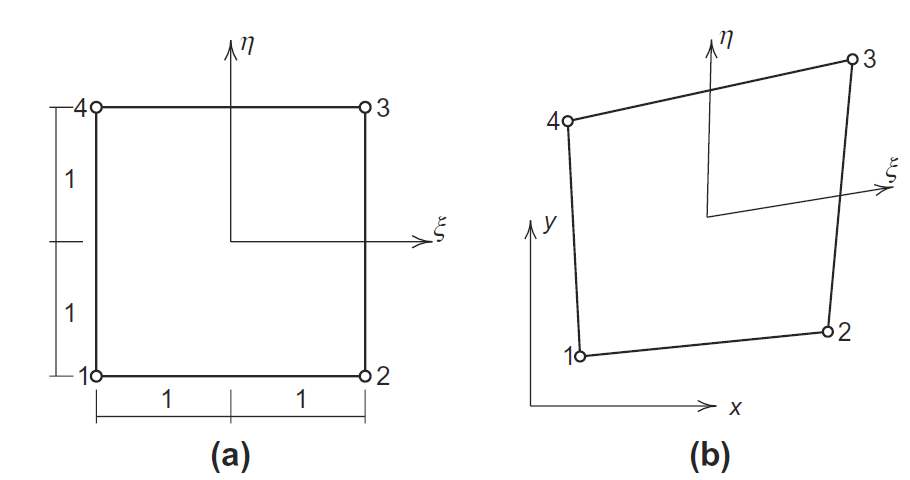
\includegraphics[width=0.75\linewidth]{files/Taylor_isoQuad-dd0d3f705ca586fcae525e52fc9aa017.png}
\caption[]{Abbildung des Elternelementes auf die reale Geometrie (\cite{zienkiewicz2005finite}).}
\label{IsoparamtericMapping}
\end{figure}

Die Abbildung des Elternelementes auf die reale Geometrie entspricht einer Koordinatentransformation. Das Elternelement wird mit den Koordinaten $\xi$, $\eta$ und $\zeta$ beschrieben, während die reale Geometrie mit den Koordinaten $x$, $y$ und $z$ beschrieben wird. Die Transformation wird durch die Abbildung $\bm{x}_h = \bm{x}_h(\xi, \eta, \zeta)$ beschrieben:

\begin{equation}
\label{geometric_mapping}
\bm{x}_h = \sum_{i=1}^{n} N_I(\bm{\xi}) \hat{\bm{x}}_I
\end{equation}

Hierbei ist $\hat{\bm{x}}_I$ der Vektor der Knotenkoordinaten und $N_I(\bm{\xi})$ die Formfunktionen des Elternelementes. Die Formfunktionen sind in der Regel Lagrange-Polynome, die die Knoten des Elternelementes interpolieren. Die Formfunktionen sind somit stückweise linear, quadratisch oder kubisch, je nach Art des Elternelementes.

Wird für die Testfunktion $\delta \bm{u}_h$ und die Verschiebung $\delta\bm{u}_h$, sowie die diskrete Darstellung der Geometrie $\bm{x}_h$ der gleiche Ansatz verwendet, so spricht man von einem isoparametrischen Element:

\begin{align}
  \delta \bm{u}_h &= \sum_{I=1}^{n} N_I(\bm{\xi}) \delta \hat{\bm{u}}_I \\
  \bm{u}_h &= \sum_{i=1}^{n} N_I(\bm{\xi}) \hat{\bm{u}}_I \\
  \bm{x}_h &= \sum_{i=1}^{n} N_I(\bm{\xi}) \hat{\bm{x}}_I
\end{align}

\begin{framed}
\textbf{Abgrenzung: weitere Parameterformulierungen}\\
Neben der isoparametrischen Formulierung gibt es auch andere Parameterformulierungen:

\begin{itemize}
\item subparametrische Formulierung: Geometrie wird mit niedrigerem Polynomgrad als die Verschiebung interpoliert
\item superparametrische Formulierung: Geometrie wird mit höherem Polynomgrad als die Verschiebung interpoliert
Beide Konzepte haben sich in der Praxis nicht durchgesetzt, wobei die superparametrische generell vermieden werden sollte (keine Konvergenz sichergestellt).
\end{itemize}
\end{framed}

\subsubsection{Berechnung der räumlichen Ableitungen}

Möchte man ein diskretisiertes Feld, z.B. $\bm{u}_h$, ableiten, so muss man über die Kettenregel die Formfunktionen ableiten:

\begin{align}
\Pd{\bm{u}_h}{\bm{x}} = \sum_{I=1}^{n} \Pd{N_I}{\bm{\xi}} \Pd{\bm{\xi}}{\bm{x}}  \hat{\bm{u}}_I \;.
\end{align}

In dieser Gleichung ist $\Pd{\bm{\xi}}{\bm{x}}$ jedoch unbekannt. Über die parametrische Darstellung der Geometrie (\ref{geometric_mapping}) kann man jedoch die Ableitung $\Pd{\bm{\xi}}{\bm{x}}$ berechnen:
\begin{align}
\bm{J} := \Pd{\bm{x}}{\bm{\xi}} & = \begin{pmatrix}
\Pd{x}{\xi} & \Pd{x}{\eta} & \Pd{x}{\zeta} \\
\Pd{y}{\xi} & \Pd{y}{\eta} & \Pd{y}{\zeta} \\
\Pd{z}{\xi} & \Pd{z}{\eta} & \Pd{z}{\zeta} 
\end{pmatrix}
=  \sum_{I=1}^{n} \Pd{N_I}{\bm{\xi}} \hat{\bm{x}}_I \\
\Rightarrow \Pd{\bm{\xi}}{\bm{x}} & = \bm{J}^{-1} \; .
\end{align}
Hier wurde die \textbf{Jacobi-Matrix} $\bm{J}$ eingeführt. Zur Berechnung der räumlichen Ableitungen der Formfunktionen werden diese einfach mit der inversen Jacobi-Matrix multipliziert:

\begin{equation}
\label{ableitungFormfunktion_03}
\Pd{N_I}{\bm{x}} = \Pd{N_I}{\bm{\xi}} \Pd{\bm{\xi}}{\bm{x}} = \Pd{N_I}{\bm{\xi}} \bm{J}^{-1} \; .
\end{equation}

\begin{framed}
\textbf{Bedeutung der Jacobi-Matrix}\\
Die Determinante der Jacobi-Matrix $\det(\bm{J})$ wird als \textbf{Jacobian} bezeichnet und stellt ein wichtiges Ma$\beta$ für die Qualität der Elementform dar. Eine Jacobi-Determinante von Null bedeutet, dass die Elementform singulär ist und die Ableitung der Formfunktionen nicht mehr eindeutig definiert ist. Es ist daher wichtig, dass die Jacobi-Determinante in dem gesamten Element positiv ist. Eine Jacobi-Determinante in der Nähe von 1 ist ideal, während Werte weit von 1 entfernt auf verzerrte Elemente hinweisen. Negative Werte der Jacobi-Determinante sind ebenfalls problematisch und sollten vermieden werden. Hier hat sich das Element selbst durchdrungen. Solche Elemente fügen dem System Energie hinzu und verfälschen die Lösung ma$\beta$geblich.
\end{framed}

\subsubsection{Anforderungen an den Finite-Elemente-Ansatz}

Um die Finite-Elemente-Methode (FEM) effektiv anzuwenden, müssen die Formfunktionen bestimmte Anforderungen erfüllen:

\textbf{Kontinuität}:

Die Formfunktionen müssen im gesamten Bereich stetig vom Grad $C^{n -1}$ sein, wobei $n$ die höchste Ableitung ist, die in der schwachen Formulierung (\ref{weakform_03}) vorkommt. Beispielsweise erfordert die Elastizitätstheorie $n=1$, was bedeutet, dass der Ansatz $C^0$-stetig sein muss. Insbesondere muss diese Stetigkeit über die Elementgrenzen hinweg gewährleistet sein. Beim Balkenelement trat die Krümmung (2. Ableitung der Durchbiegung) in der schwachen Form auf. Deshalb muss der Ansatz für das Balkenelement $C^1$-stetig sein.

\textbf{Vollständigkeit}:

Die Formfunktionen müssen die exakte Lösung approximieren können, wenn die Anzahl der Elemente gegen unendlich geht. Dies stellt sicher, dass die numerische Lösung mit zunehmender Verfeinerung des Netzes immer genauer wird.

\textbf{Eindeutigkeit}:

Die Formfunktionen müssen eindeutig sein, d.h., es darf keine lineare Abhängigkeit zwischen den Formfunktionen geben. Diese Eigenschaft ist entscheidend, um sicherzustellen, dass die Lösung der Gleichungen eindeutig bestimmt ist.

Diese Anforderungen sind essenziell, um die Genauigkeit und Zuverlässigkeit der FEM-Lösungen zu gewährleisten. Sie stellen sicher, dass die numerischen Ergebnisse physikalisch sinnvoll und mathematisch korrekt sind und dass die Methode gegen die analytische Lösung konvergiert.

Für diese drei Anforderungen existiert auch eine ingenieurmä$\beta$ige Deutung, die im Folgenden beschrieben wird.

\begin{figure}[!htbp]
\centering
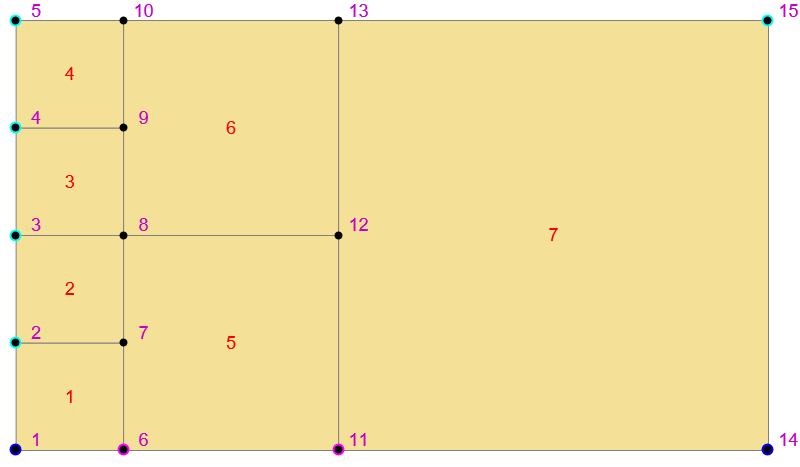
\includegraphics[width=0.75\linewidth]{files/NonConforming_Mesh_0-a479aa456cf524d92a168b6991747316.png}
\caption[]{Verletzung der Stetigkeitsanforderung in der Finite-Elemente-Methode.}
\label{Stetigkeit_01}
\end{figure}

Die Forderung der Stetigkeit über die Elementgrenzen hinweg wird über eine konforme Vernetzung sichergestellt. Ein typisches Beispiel zur Veranschaulichung dieser Anforderung ist die Elementierung mit 4-Knoten-Rechteckelementen. Betrachten wir eine eingespannte Scheibe, die einer Zugbelastung ausgesetzt ist. Um die Schnittkräfte genauer zu erfassen, wird das Netz in Richtung der Einspannung verfeinert. Dies soll die Behinderung der Querkontraktion besser erfassen. Allerdings führt diese Netzverfeinerung in einigen Fällen zu unzulässigen Klaffungen im deformierten Netz.

Die Ursache für diese unzulässigen Klaffungen liegt in der Zuordnung der Knoten zu den Elementen. In diesem Beispiel werden die Knoten 7, 9 und 12 nur zu zwei Elementen zugeordnet. Die Elementkante von Element 5, 6 und 7 wird nicht an die Deformation der genannten Knoten gekoppelt. Diese fehlerhafte Zuordnung führt dazu, dass die Schnittkräfte in der Nähe von Inkompatibilitäten nicht korrekt berechnet werden.

\begin{figure}[!htbp]
\centering
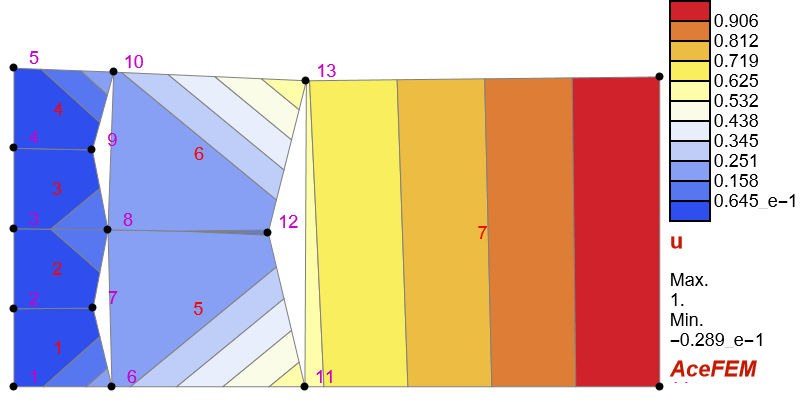
\includegraphics[width=0.75\linewidth]{files/NonConforming_Mesh_0-d55b1d7d132d2ca41b6cb0a474d78e2a.png}
\caption[]{Verschiebungsfeld bei einer nicht-konformen Netzstruktur.}
\label{Stetigkeit_02}
\end{figure}

Diese lokalen Störungen klingen jedoch mit ausreichend gro$\beta$em Abstand ab, wie es das Prinzip von St. Venant beschreibt. Dieses Prinzip besagt, dass die Auswirkungen von lokalen Unregelmä$\beta$igkeiten in der Belastung oder Geometrie mit zunehmendem Abstand von der Störungsquelle abnehmen. Daher sind die Auswirkungen der Inkompatibilitäten auf die Gesamtlösung begrenzt.

Ein weiterer Fehler, der bei der Vernetzung entstehen kann, ist die Verwendung von Elementen mit unterschiedlicher Elementordnung.

\begin{figure}[!htbp]
\centering
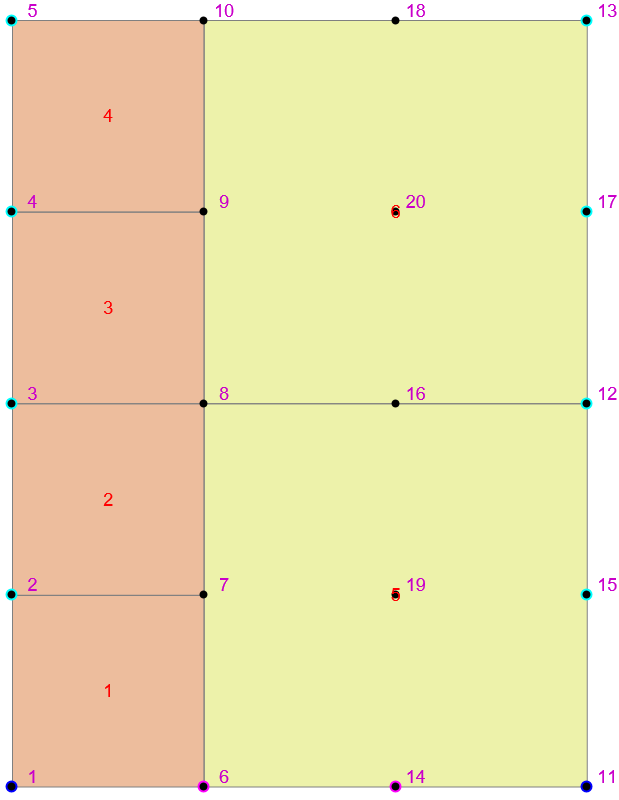
\includegraphics[width=0.5\linewidth]{files/NonConforming_Mesh_0-60bcd99bf5156e972d558f9ec97d5e1f.png}
\caption[]{Verletzung der Stetigkeitsanforderung in der Finite-Elemente-Methode durch Verwendung von Elementen mit unterschiedlicher Ordnung.}
\label{Stetigkeit_03}
\end{figure}

Auch hier ist die resultierende Verschiebung nicht korrekt. Eigentlich sollte die Verschiebung linear sein, was jedoch nicht der Fall ist.

\begin{figure}[!htbp]
\centering
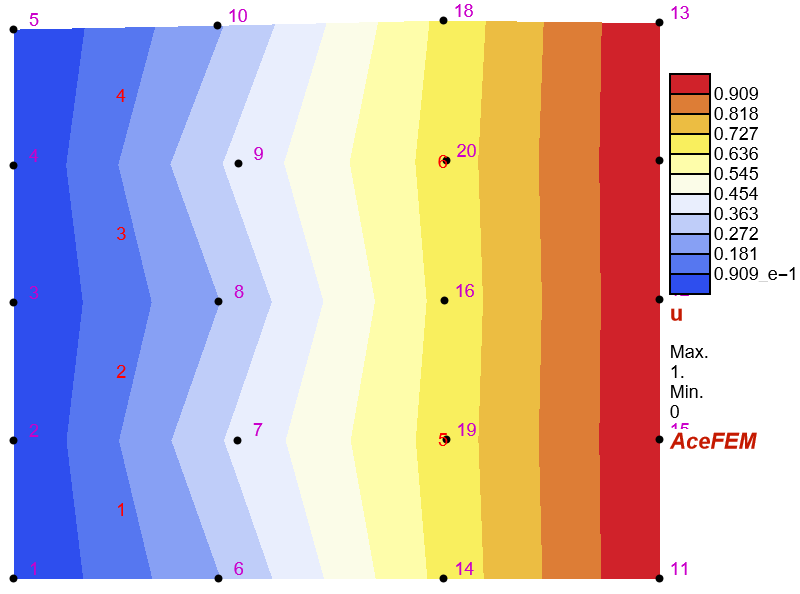
\includegraphics[width=0.75\linewidth]{files/NonConforming_Mesh_0-3212f5420fe42526cc08f008921dce3a.png}
\caption[]{Verletzung der Stetigkeitsanforderung in der Finite-Elemente-Methode durch Verwendung von Elementen mit unterschiedlicher Ordnung - Resultierendes Verschiebungsfeld.}
\label{Stetigkeit_04}
\end{figure}

Die Stetigkeitsanforderung ist von gro$\beta$er praktischer Bedeutung, da sie sicherstellt, dass die numerische Lösung physikalisch sinnvoll und mathematisch korrekt ist. Eine konforme Vernetzung, bei der die Knoten korrekt zugeordnet sind, ist entscheidend, um die Genauigkeit der FEM-Lösungen zu gewährleisten.

Um eine lokale Verfeinerung zu erzielen, kann man entweder spezielle Elemente verwenden (bei denen die entsprechenden Knoten angelegt wurden) oder man fügt eine entsprechende Zwischenschicht, wie in Abbildung Figure~\ref{Stetigkeit_05}, ein.

\begin{figure}[!htbp]
\centering
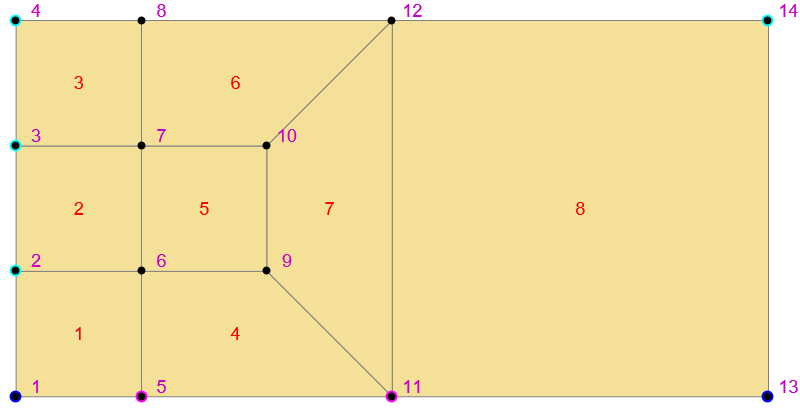
\includegraphics[width=0.75\linewidth]{files/Conforming_Mesh_01-ed2fc9715e8d4d760dd08d09cc38aea6.png}
\caption[]{Übergangselementschicht zur lokalen Verfeinerung.}
\label{Stetigkeit_05}
\end{figure}

Hierbei wird das Verschiebungsfeld durch die Zwischenschicht korrekt wiedergegeben.

\begin{figure}[!htbp]
\centering
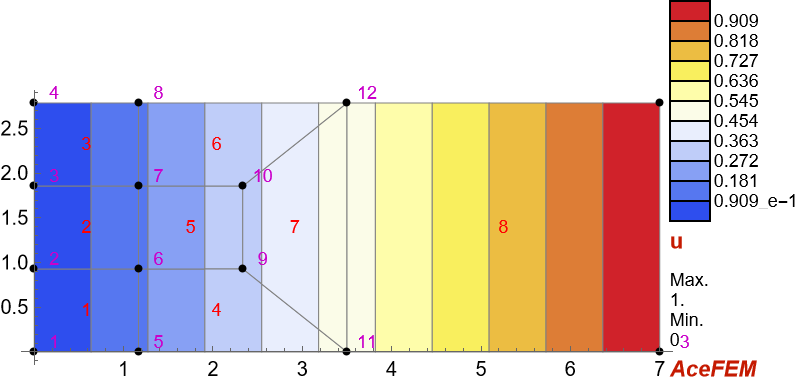
\includegraphics[width=0.75\linewidth]{files/Conforming_Mesh_02-1dadb7235cd7cceba4d6c6f0972ddf3e.png}
\caption[]{Übergangselementschicht zur lokalen Verfeinerung - Verschiebungsfeld.}
\label{Stetigkeit_06}
\end{figure}

Ein zentraler Aspekt der Vollständigkeit in der Finite-Elemente-Methode ist die Fähigkeit, Starrkörperverschiebungen darzustellen. Die Starrkörperverschiebung $\bm{u}_c = \bm{c}$ muss durch die Ansatzfunktionen $\bm{N}_I(\bm{\xi})$ exakt wiedergegeben werden können. Der mathematische Ausdruck dafür ist:
\begin{align}
\bm{u}_c & = \sum_{I=1}^{n} N_I(\bm{\xi}) \hat{\bm{u}}_I  = \sum_{I=1}^{n} N_I(\bm{\xi}) {\bm{c}} = \bm{c} \sum_{I=1}^{n} N_I(\bm{\xi}) \\
\Rightarrow \qquad 1 &= \sum_{I=1}^{n} N_I(\bm{\xi}) 
\end{align}

Diese Eigenschaft wird in der Literatur als \textbf{Partitions of Unity} bezeichnet. Die praktische Relevanz dieser Eigenschaft liegt darin, dass in Tragstrukturen die Lösung in einen Anteil der Starrkörperverschiebung und einen Anteil, der Dehnungen hervorruft, aufgeteilt werden kann. Ein Beispiel hierfür ist ein Balken: Am freien Ende ist die Verschiebung am grö$\beta$ten, der Balken jedoch erfährt hier am wenigsten Dehnung. Eine praktische Überprüfung besteht darin, dass Starrkörperverschiebungen keine Dehnungen/Spannungen hervorrufen dürfen.

Ein weiteres Beispiel zur Überprüfung der Vollständigkeit ist die Darstellbarkeit konstanter Dehnungszustände (Patch-Test). Ist ein Element in der Lage, einen konstanten Dehnungszustand darzustellen, so ist auch ein praktischer Nachweis der Konvergenz der Elementformulierung bei Verfeinerung der Vernetzung gegeben. Dies kann man sich einfach am Beispiel in Abbildung Figure~\ref{KonvergenzPatchtest} verdeutlichen. Hier werden die Schnittkräfte in einen konstanten Anteil und einen linear veränderlichen unterteilt. Mit steigender Elementanzahl wird der konstante Term der Schnittkraft dominant und ist somit der ma$\beta$gebliche Anteil für die Konvergenz.

\begin{figure}[!htbp]
\centering
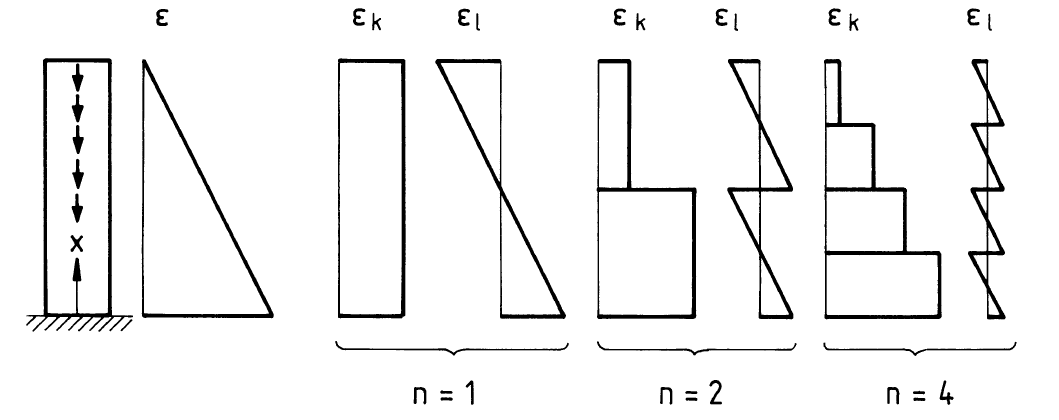
\includegraphics[width=0.75\linewidth]{files/Knothe_02-eea4e4a5abfe3ac959c4e32cca1a63d8.png}
\caption[]{Mit steigender Elementanzahl wird der konstante Term der Schnittkraft dominant (\cite{knothe1991finite}).}
\label{KonvergenzPatchtest}
\end{figure}

\begin{framed}
\textbf{Fragen zum Kapitel}\\
\textbf{Isoparametrische FEM}

\begin{itemize}
\item Welche Aussagen sind zutreffend?\begin{itemize}
\item Bei der isoparametrischen FEM wird die schwache Form auf einem uniformen Elternelement gebildet und danach auf die reale Geometrie transformiert.
\item Bei der isoparametrischen FEM werden die gleichen Ansätze bezüglich Geometrie und Verschiebung gewählt.
\item Bei der subparametrischen FEM wird die Geometrie mit einem niedrigeren Polynomgrad als die Verschiebung approximiert.
\item Nur die isoparametrische FEM ist gesichert konvergent.
\end{itemize}


\item Über welches Ma$\beta$ kann man die Qualität eines FE-Netzes quantifizieren?
\item Ist ein Element mit einer Jacobi-Determinante $\det \boldsymbol{J} < 0$ für die Berechnung zulässig?
\item Welche Anforderungen muss ein Finite-Element-Ansatz erfüllen, damit die Lösung gegen die analytische Lösung konvergiert?
\item Wie kann man die Forderung der Kontinuität des Ansatzes bei der Vernetzung verletzen?
\item Warum ist es wichtig, dass ein Finites Element Starrkörperverschiebungen korrekt darstellt?
\item Was ist ein Patch-Test? Was wird damit untersucht?
\item Was bedeutet der Begriff \textit{Partition of Unity}?
\end{itemize}
\end{framed}

\subsubsection{Ansatzfunktionen}

Um verzerrungsfreie Starrkörperbewegungen sowie konstante Verzerrungszustände beschreiben zu können und dabei ein räumlich isotropes Verformungsverhalten zu approximieren, müssen die Ansatzfunktionen vollständig sein.
Für ein ebenes Dreieckselement bedeutet dies z.B.
\begin{align}
u(\xi,\eta) &= \underbrace{\underbrace{ a_1 + a_2 \xi + a_3 \eta}_{\text{3 Knoten Dreieck}} + a_4 \xi^2 + a_5 \eta^2 + a_6 \xi \eta}_{\text{6 Knoten Dreieck}} \; .
\end{align}
Hier sind für ein 3-Knoten-Dreieckselement alle linearen Terme enthalten, für ein 6-Knoten-Dreieckselement sind auch die quadratischen und bilinearen Terme enthalten.
Illustriert kann man sich am besten ein pascalsches Dreieck wie in Abbildung Figure~\ref{pascaltriangle} vorstellen.

\begin{figure}[!htbp]
\centering
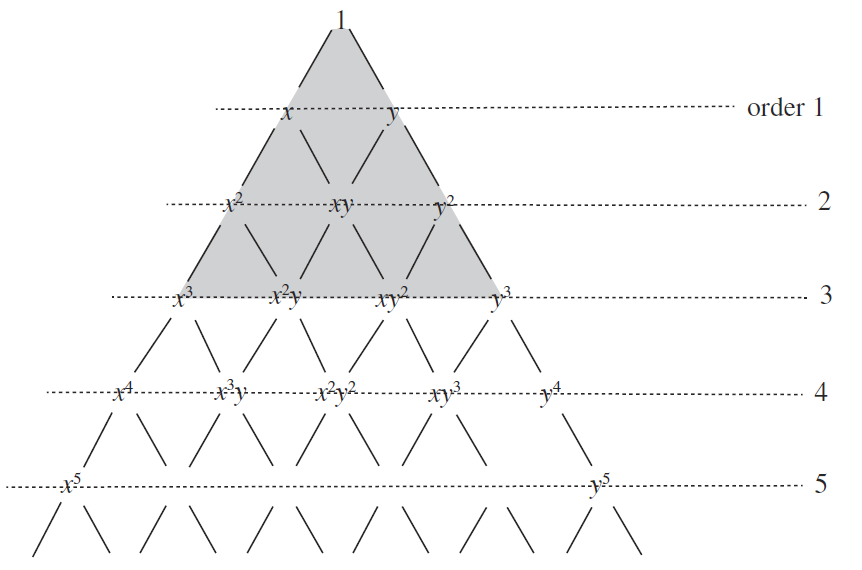
\includegraphics[width=0.45\linewidth]{files/Taylor_PascalTriangl-d58874fb2e0793428871a0933d31951f.png}
\caption[]{Pascal'sches Dreieck für Dreieckselemente (\cite{zienkiewicz2005finite})}
\label{pascaltriangle}
\end{figure}

Analog kann dazu ein vollständiges Viereckselement definiert werden:
\begin{align}
u(\xi,\eta) &= \underbrace{\underbrace{ a_1 + a_2 \xi + a_3 \eta + a_4 \xi \eta}_{\text{4 Knoten Viereck}} + a_5 \xi^2 + a_6 \eta^2 + a_7 \xi^2 \eta + a_8 \xi \eta^2}_{\text{8 Knoten Viereck}} \; .
\end{align}

Auch hier liefert das Pascalsche Dreieck eine anschauliche Interpretation:

\begin{figure}[!htbp]
\centering
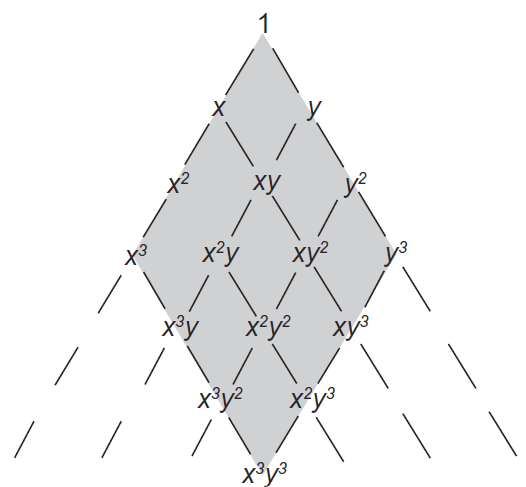
\includegraphics[width=0.45\linewidth]{files/Taylor_PascalQuad-53f0990e72ee0826eb02b4d26ee4606a.png}
\caption[]{Pascalsches Dreieck für Rechteckelemente (\cite{zienkiewicz2005finite}). Grau unterlegt ist ein kubisches Rechteckelement.}
\label{pascalQuad}
\end{figure}

\paragraph{Formfunktionen für $C^0$-Elemente}

Nachfolgend werden kurz die Ansatzfunktionen für 1D-, 2D- und 3D-Elemente mit Lagrange-Polynomen vorgestellt:

\subparagraph{1D Formfunktionen}

\begin{figure}[!htbp]
\centering
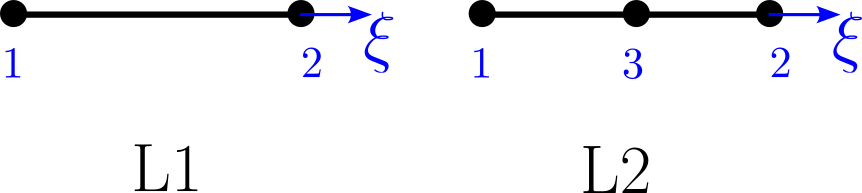
\includegraphics[width=0.625\linewidth]{files/Line-Elements-e2d4de7bd279c40b8dc47f1c98a894a5.png}
\caption[]{1D-Elemente mit linearer und quadratischer Ansatzfunktion}
\label{linearElements}
\end{figure}

Für den linearen Fall haben 1D-Elemente 2 Knoten und damit 2 Formfunktionen:

\begin{align}
N_1 &= \frac{1}{2} (1 - \xi) & N_2 &= \frac{1}{2} (1 + \xi)
\end{align}

Für den quadratischen Fall haben 1D-Elemente 3 Knoten und damit 3 Formfunktionen:
\begin{align}
N_1 &= \frac{1}{2} \xi (\xi - 1) & N_2 &= 1 - \xi^2 & N_3 &= \frac{1}{2} \xi (\xi + 1)
\end{align}

%  ```{figure} images/Shapefunctions_1d.png
% ---
% name: Shapefunctions_1dd
% alt: Formfunktionen für 1D-Elemente
% width: 500px
% ---
% Formfunktionen für 1D-Elemente
% ```

\subparagraph{2D Formfunktionen}

\begin{figure}[!htbp]
\centering
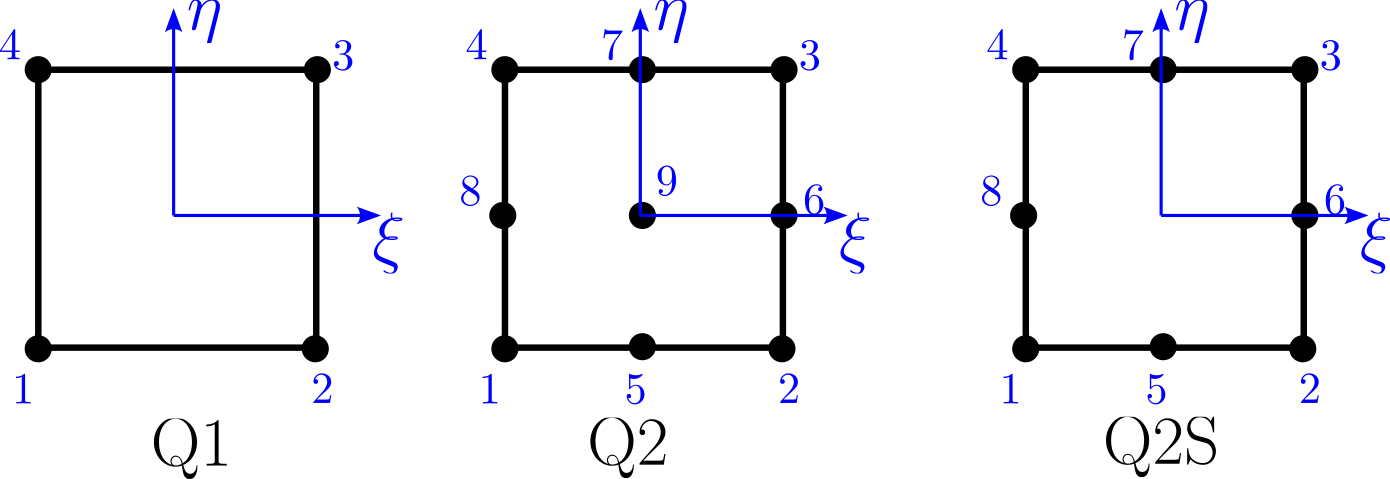
\includegraphics[width=0.625\linewidth]{files/QuadElements-3c42e67cc9a797973b3fd3afce627f44.png}
\caption[]{2D-Rechteck-Elemente mit linearer und quadratischer Ansatzfunktion}
\label{quadElements}
\end{figure}

Im 2D-Fall werden die Formfunktionen für Rechteck-Elemente als Tensorprodukt der 1D-Formfunktionen definiert. Für ein 2D-Rechteck-Element mit 4 Knoten (lineares Element) sind die Formfunktionen:

\begin{align}
N_1 &= \frac{1}{4} (1 - \xi)(1 - \eta) & N_2 &= \frac{1}{4} (1 + \xi)(1 - \eta) \\
N_3 &= \frac{1}{4} (1 + \xi)(1 + \eta) & N_4 &= \frac{1}{4} (1 - \xi)(1 + \eta)
\end{align}

\begin{figure}[!htbp]
\centering
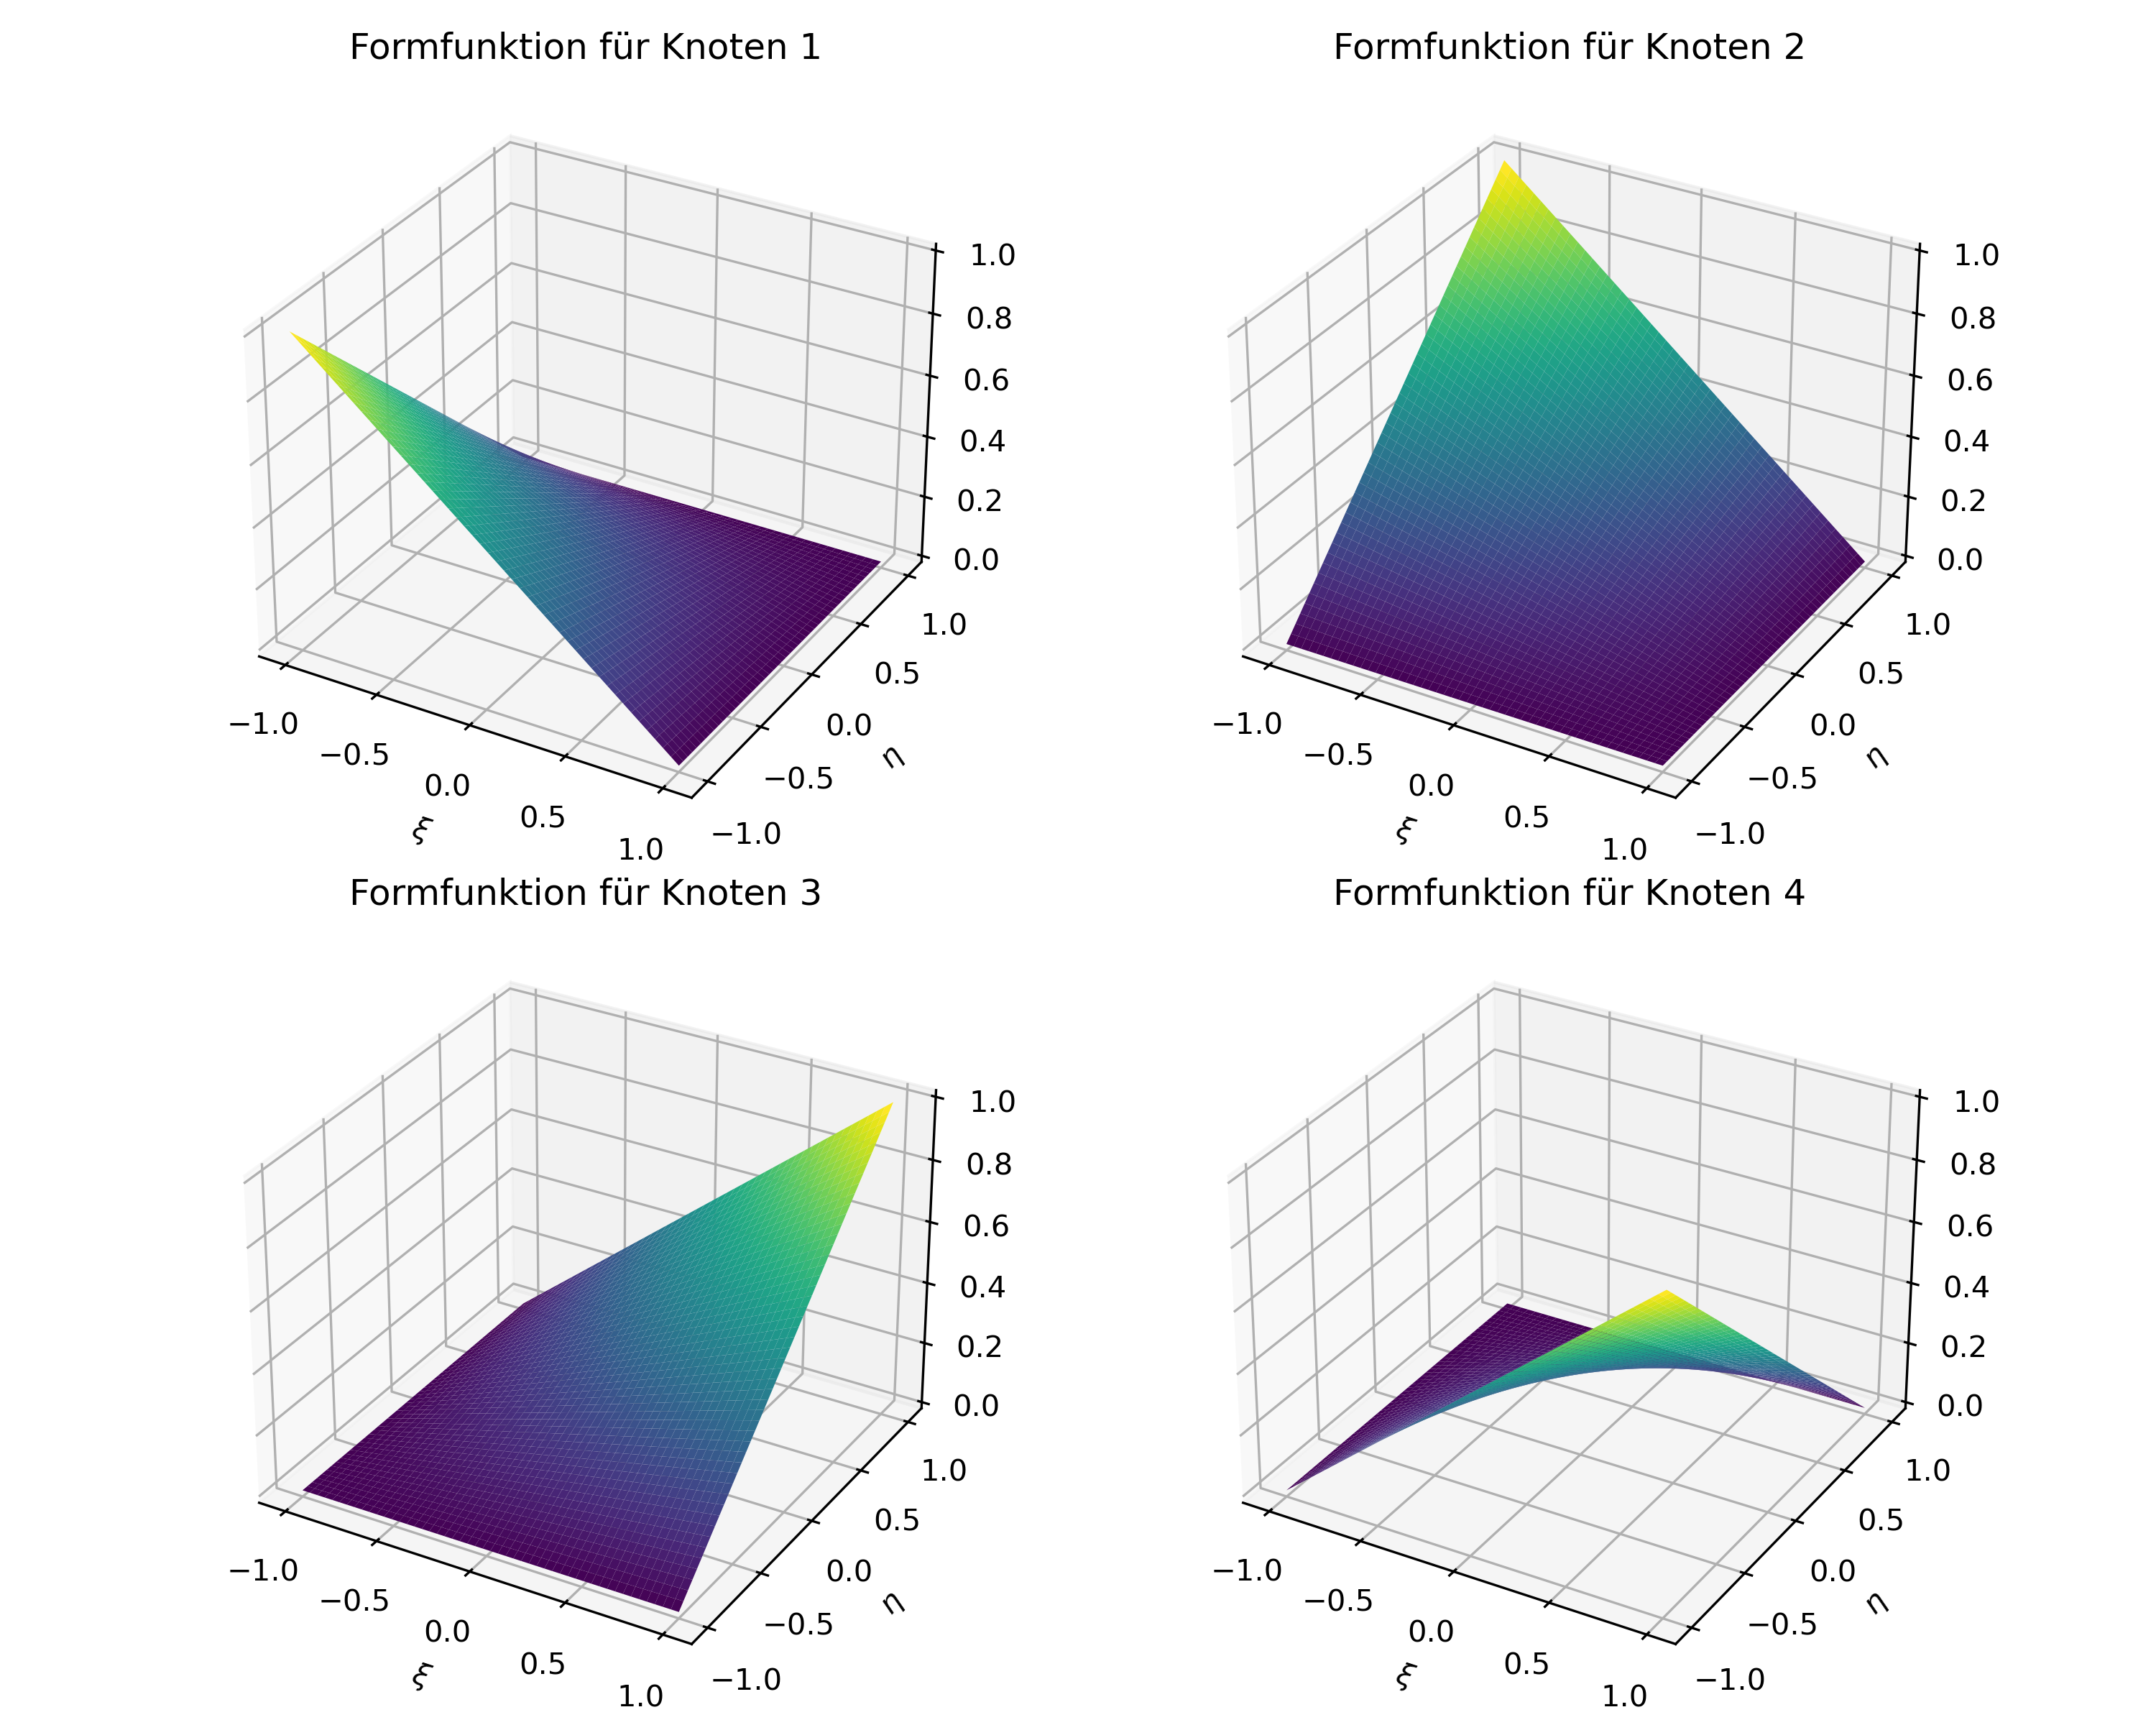
\includegraphics[width=0.625\linewidth]{files/shape_functions_Q4-1dbb3a2b8195bdb03c9a69d2f5a12df5.png}
\caption[]{Bilineare Formfunktionen für 2D-Rechteck-Elemente.}
\label{quadElementsQ4N}
\end{figure}

Um ein vollständiges Element der Ordnung 2 zu erhalten, benötigt man 9 Knoten beim Rechteck-Element. Die entsprechenden Formfunktionen lauten:

\begin{align*}
N_1 &= \frac{1}{4} \xi \eta (\xi - 1)(\eta - 1) & N_2 &= \frac{1}{2} (1 - \xi^2) (1 - \eta) \\
N_3 &= \frac{1}{4} \xi \eta (\xi + 1)(\eta - 1) & N_4 &= \frac{1}{2} (1 + \xi) (1 - \eta^2) \\
N_5 &= \frac{1}{4} \xi \eta (\xi + 1)(\eta + 1) & N_6 &= \frac{1}{2} (1 - \xi^2) (1 + \eta) \\
N_7 &= \frac{1}{4} \xi \eta (\xi - 1)(\eta + 1) & N_8 &= \frac{1}{2} (1 - \xi) (1 - \eta^2) \\
N_9 &= (1 - \xi^2)(1 - \eta^2)
\end{align*}

\begin{figure}[!htbp]
\centering
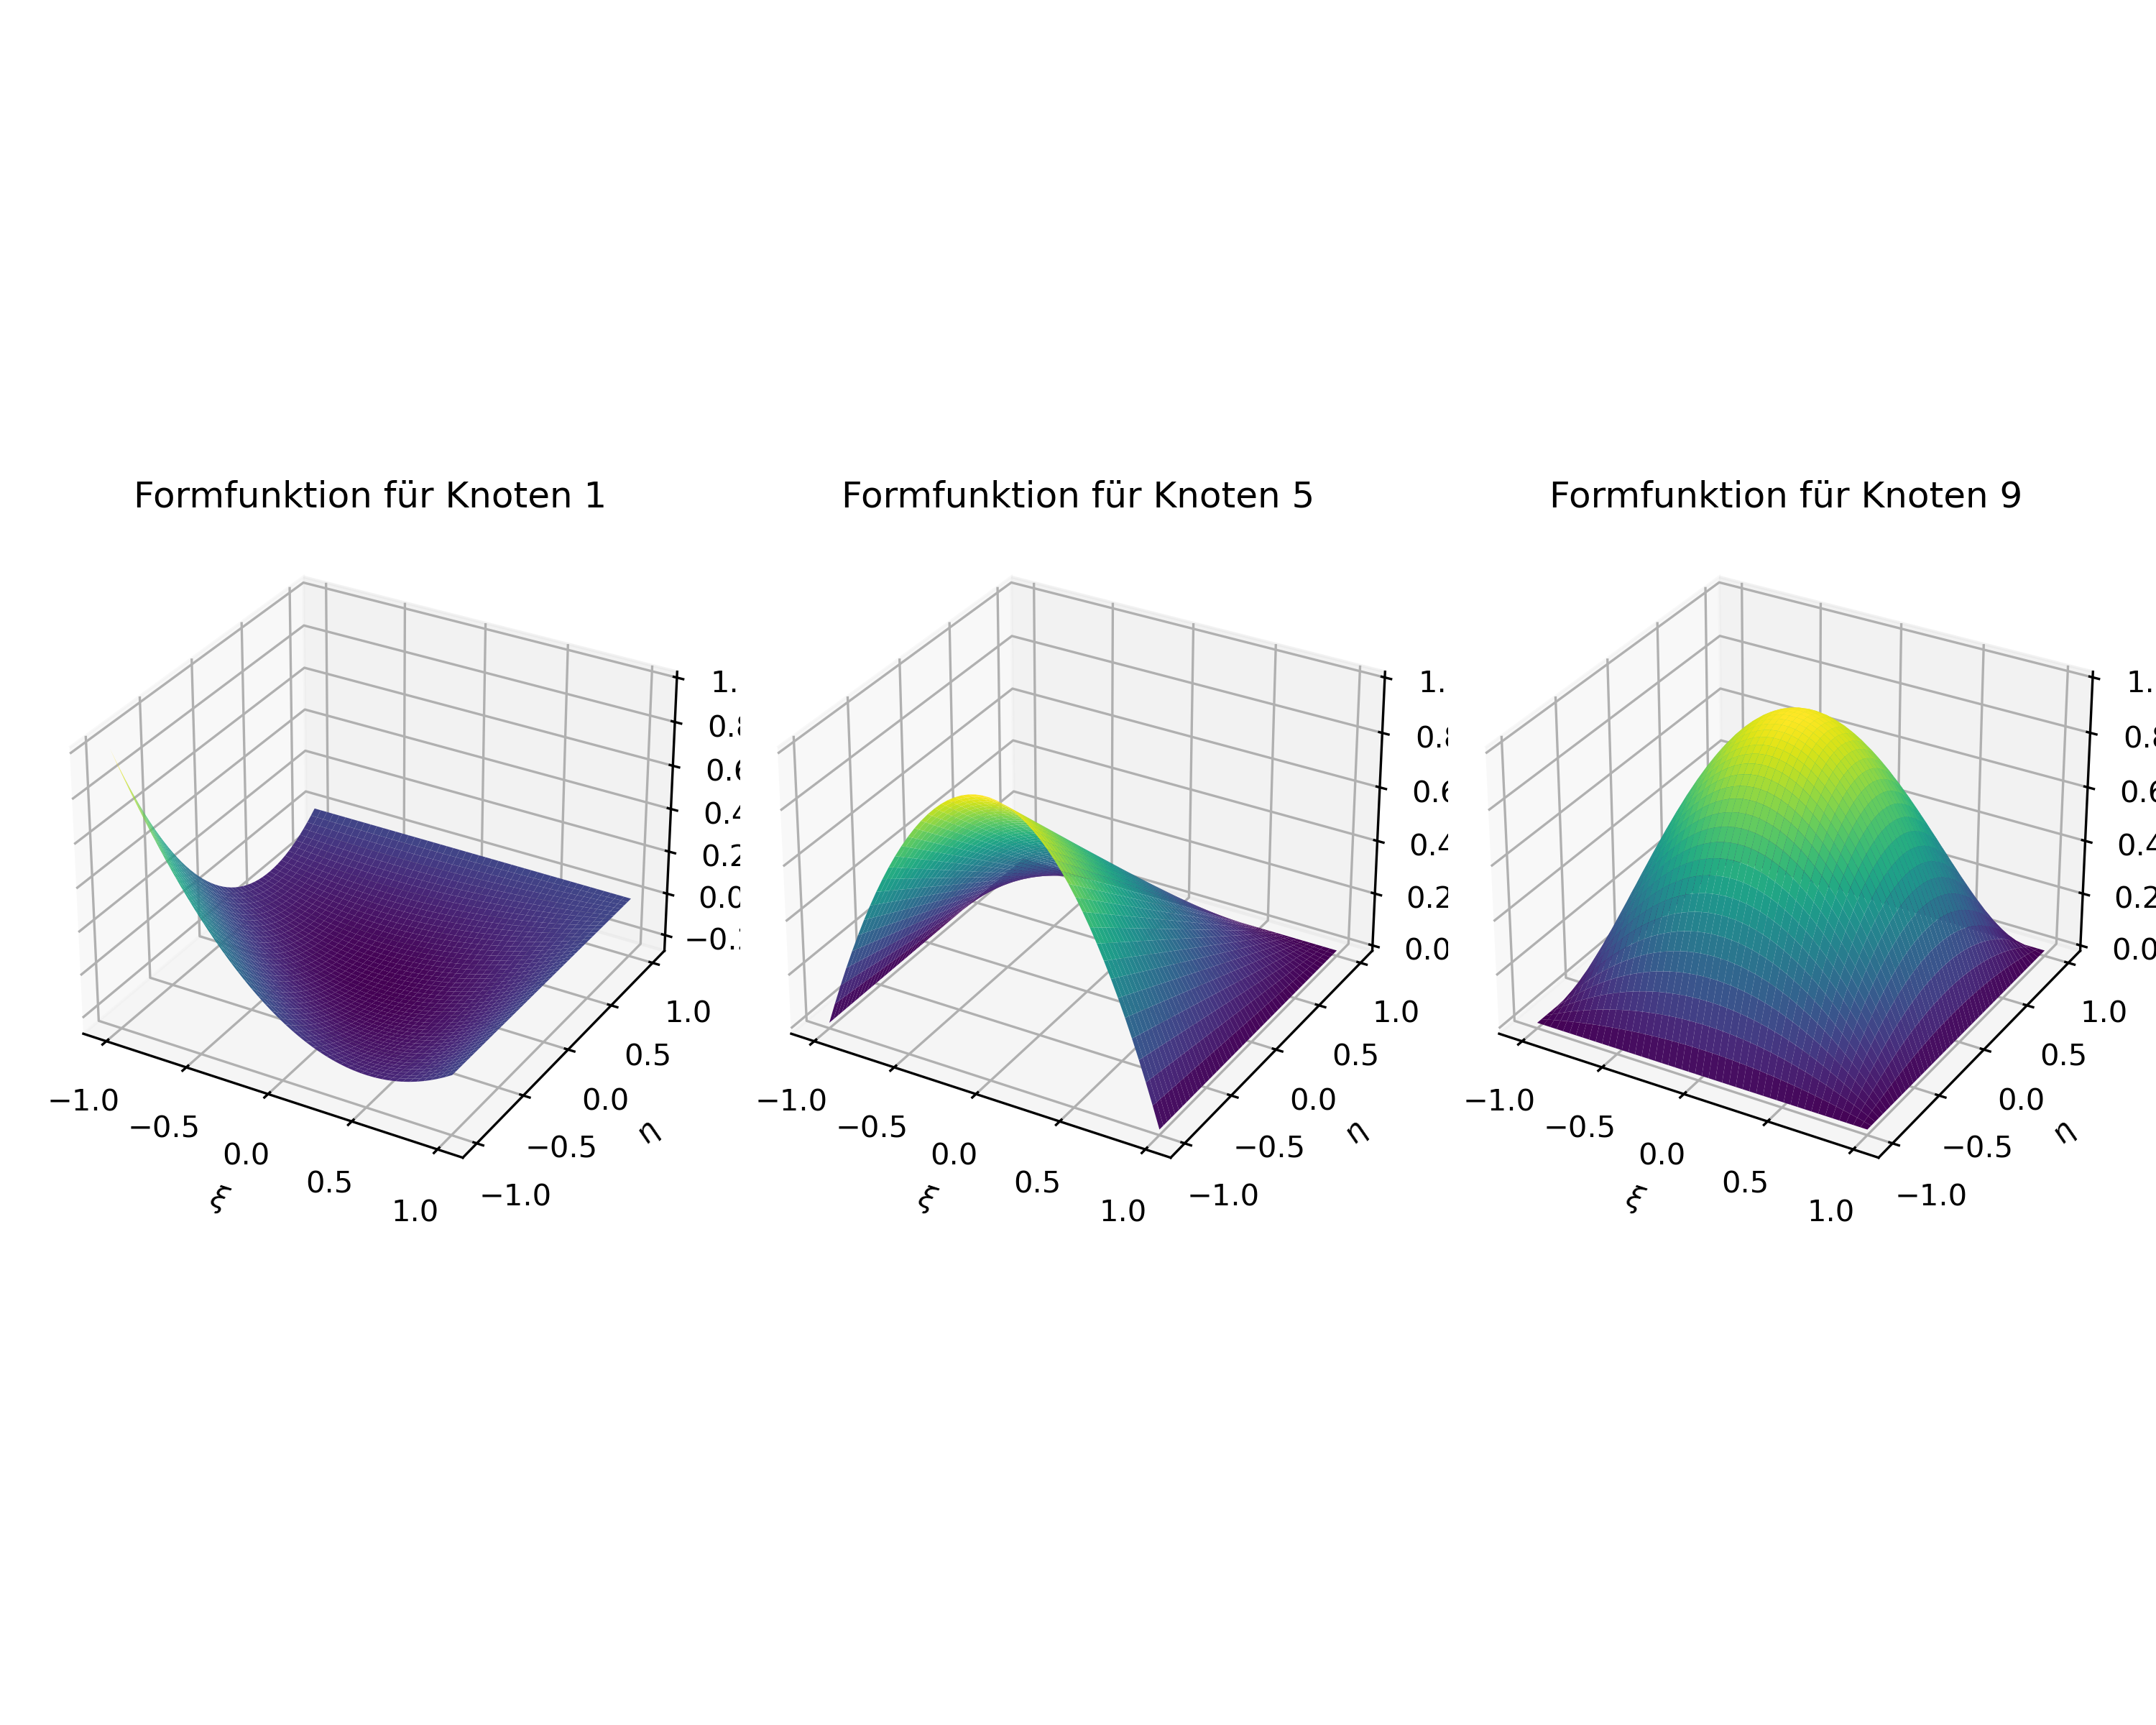
\includegraphics[width=0.625\linewidth]{files/shape_functions_Q9-4b92558abd04628eb843f07d85382fbd.png}
\caption[]{Biquadratische Formfunktionen für 2D-Rechteck-Elemente (Q2).}
\label{quadElementsQ9N}
\end{figure}

In der Praxis der Finite-Elemente-Methode beschränkt man sich jedoch nicht ausschlie$\beta$lich auf Q9-Elemente, die die vollständige Polynomordnung 2 aufweisen, wie in Abbildung Figure~\ref{pascalQuad} dargestellt. Serendipity-Elemente sind im oben beschriebenen Sinne nicht vollständig, erfüllen jedoch die Anforderungen an die räumliche Isotropie, die Verzerrungsfreiheit bei Starrkörperbewegungen und die Abbildung konstanter Verzerrungszustände. Der Begriff „Serendipity`` geht vermutlich auf ein Märchen von H. Walpole, „Die drei Prinzen von Serendip``, zurück, in dem die Prinzen die Fähigkeit besitzen, durch Zufall unverhoffte und glückliche Entdeckungen zu machen. Das zugehörige Element ist in Abbildung Figure~\ref{quadElements} als \textbf{Q2S} dargestellt. Die Ansatzfunktionen lauten:

\begin{align}
N_1(\xi ,\eta ) & =\frac{1}{4} (1-\eta ) (1-\xi ) (-\eta -\xi -1) & N_2(\xi ,\eta ) & =\frac{1}{4} (1-\eta ) (\xi +1) (-\eta +\xi -1) \\
N_3(\xi ,\eta ) & =\frac{1}{4} (\eta +1) (\xi +1) (\eta +\xi -1) & N_4(\xi ,\eta ) & =\frac{1}{4} (\eta +1) (1-\xi ) (\eta -\xi -1) \\
N_5(\xi ,\eta ) & =\frac{1}{2} (1-\eta ) \left(1-\xi ^2\right) & N_6(\xi ,\eta ) & =\frac{1}{2} \left(1-\eta ^2\right) (\xi +1)\\
N_7(\xi ,\eta ) & =\frac{1}{2} (\eta +1) \left(1-\xi ^2\right) &
N_8(\xi ,\eta ) & =\frac{1}{2} \left(1-\eta ^2\right) (1-\xi )
\end{align}

\begin{figure}[!htbp]
\centering
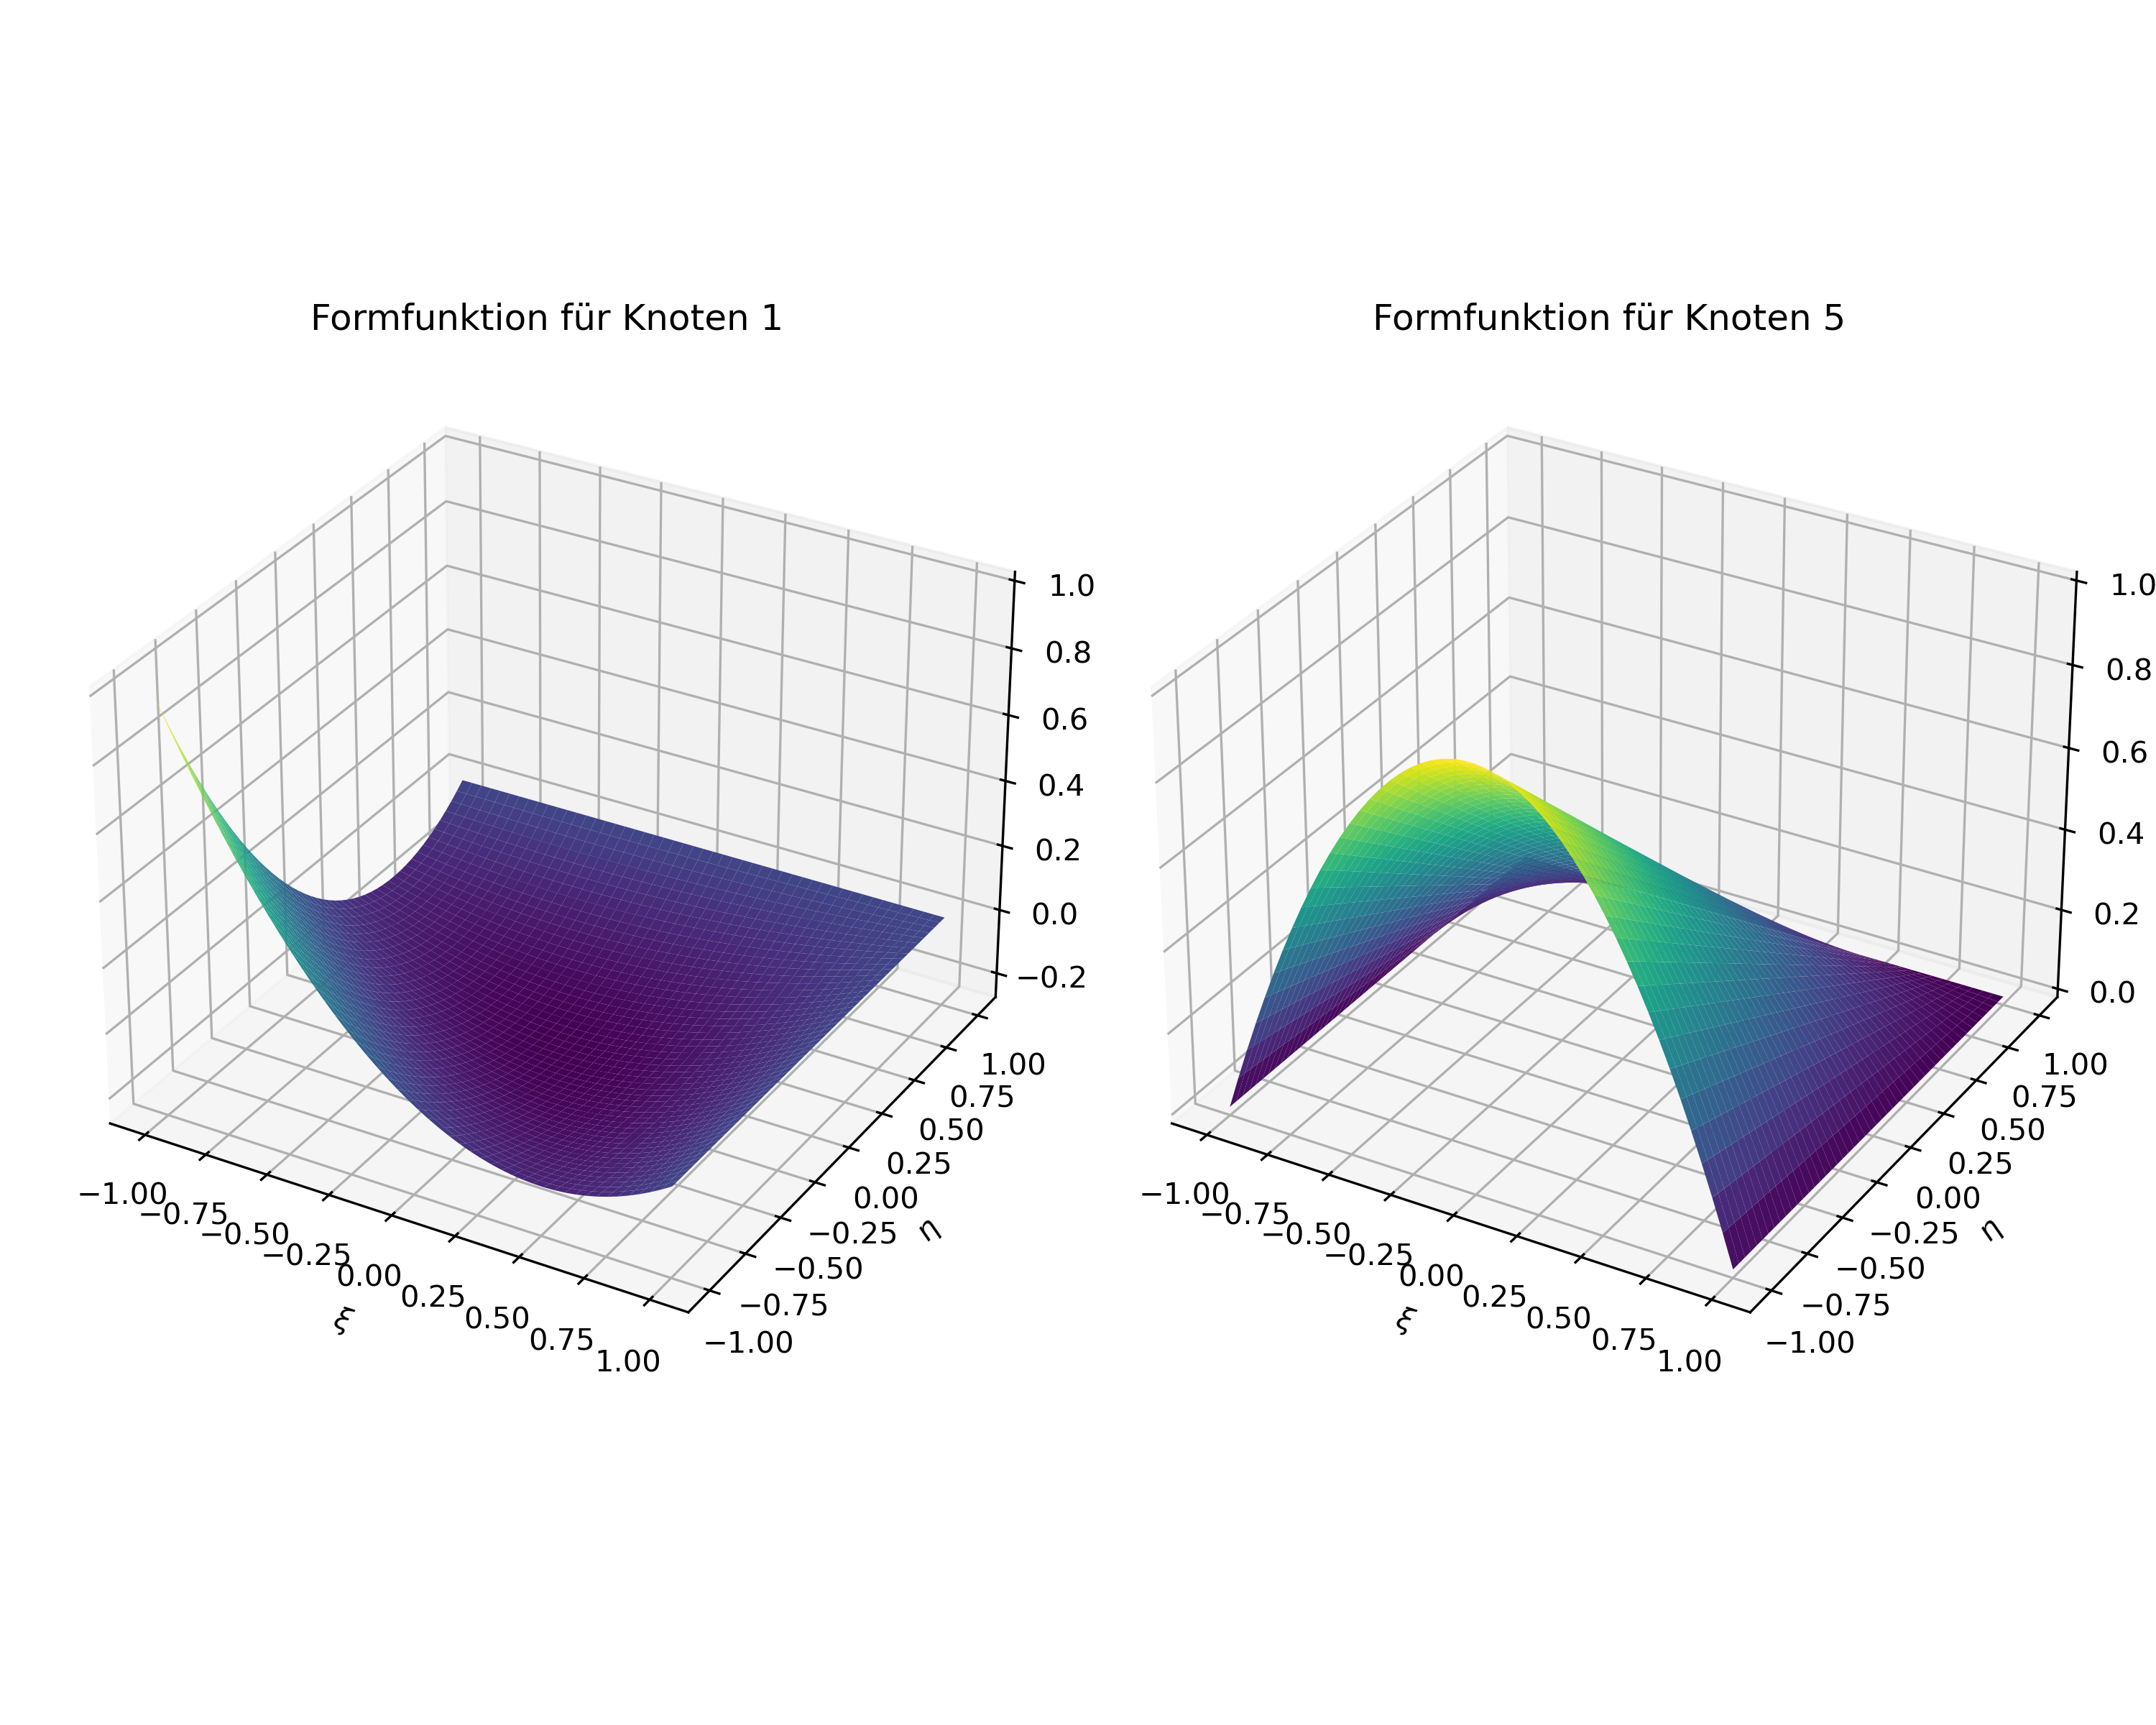
\includegraphics[width=0.625\linewidth]{files/shape_functions_Q8-48d9fa7e53fa8fe13e232d8a4fc0aa98.png}
\caption[]{Biquadratische Serendipity-Formfunktionen für 2D-Rechteck-Elemente (Q2S).}
\label{quadElementsQ8N}
\end{figure}

Eine weitere Möglichkeit der zweidimensionalen Vernetzung ist die Verwendung von Dreiecken. In den gebräuchlichen FEM-Programmen werden dabei Dreiecke mit 3 oder 6 Knoten implementiert. Diese sind in Figure~\ref{triangleElements} dargestellt.

\begin{figure}[!htbp]
\centering
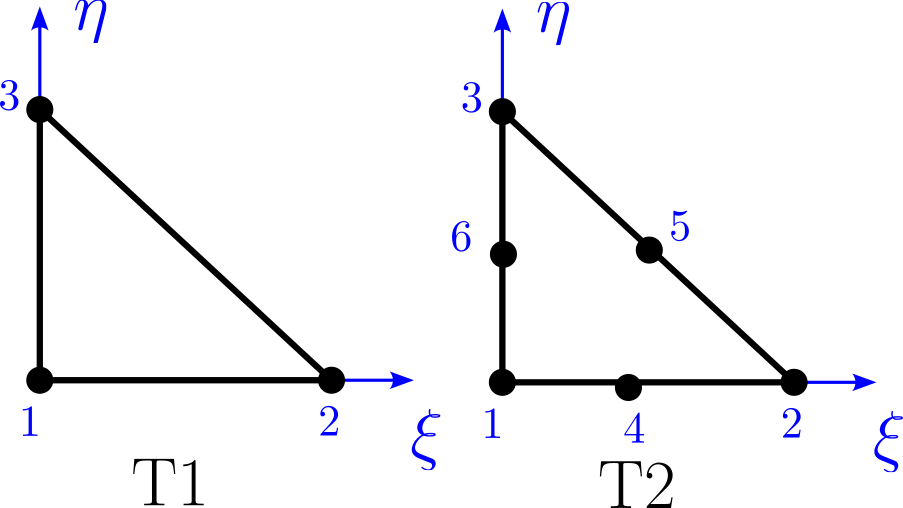
\includegraphics[width=0.625\linewidth]{files/TriangleElements-0c3b6af2501f4575008c6e8b2ea02f48.png}
\caption[]{Dreieck-Elemente mit linearen (T1) und quadratischen (T2) Formfunktionen.}
\label{triangleElements}
\end{figure}

Die linearen Dreieck-Elemente (T1) sind die einfachsten Elemente und werden in der Literatur häufig als ``konstant'' bezeichnet. Dies bezieht sich auf die abgeleiteten Grö$\beta$en (z.B. Spannungen, Dehnungen, etc.), die als konstant dargestellt werden. Die Formfunktionen lauten:

\begin{align}
\lambda & = 1 - \xi - \eta & N_1(\xi ,\eta ) & = \lambda \\
N_2(\xi ,\eta ) & = \xi & N_3(\xi ,\eta ) & = \eta
\end{align}

\begin{figure}[!htbp]
\centering
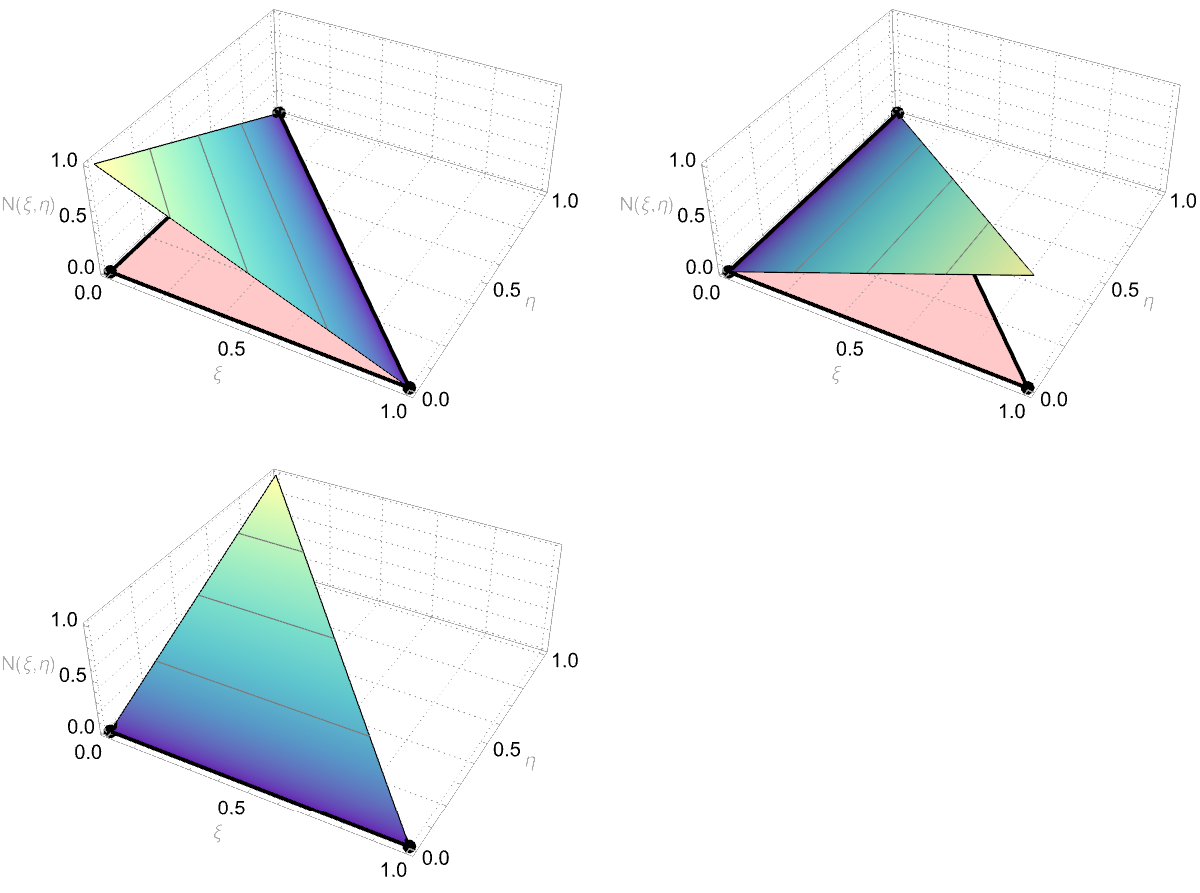
\includegraphics[width=0.625\linewidth]{files/shape_T1-594d407f8c44ecc83abb40efc728a385.png}
\caption[]{Formfunktionen für das Dreieck-Element T1.}
\label{shapefunTria}
\end{figure}

Die Formfunktionen für Dreieck-Elemente mit 6 Knoten (T2) sind vollständig quadratisch. Insgesamt hat das T2-Element bessere Approximationseigenschaften als das T1-Element. Die Formfunktionen lauten:

\begin{align}
\lambda & = 1 - \xi - \eta & N_1(\xi ,\eta ) & = \lambda (2\lambda - 1) \\
N_2(\xi ,\eta ) & = \xi (2\xi - 1) & N_3(\xi ,\eta ) & = \eta (2\eta - 1) \\
N_4(\xi ,\eta ) & = 4\lambda \xi & N_5(\xi ,\eta ) & = 4\xi \eta \\
N_6(\xi ,\eta ) & = 4\lambda \eta
\end{align}

\subparagraph{3D Formfunktionen}

\begin{figure}[!htbp]
\centering
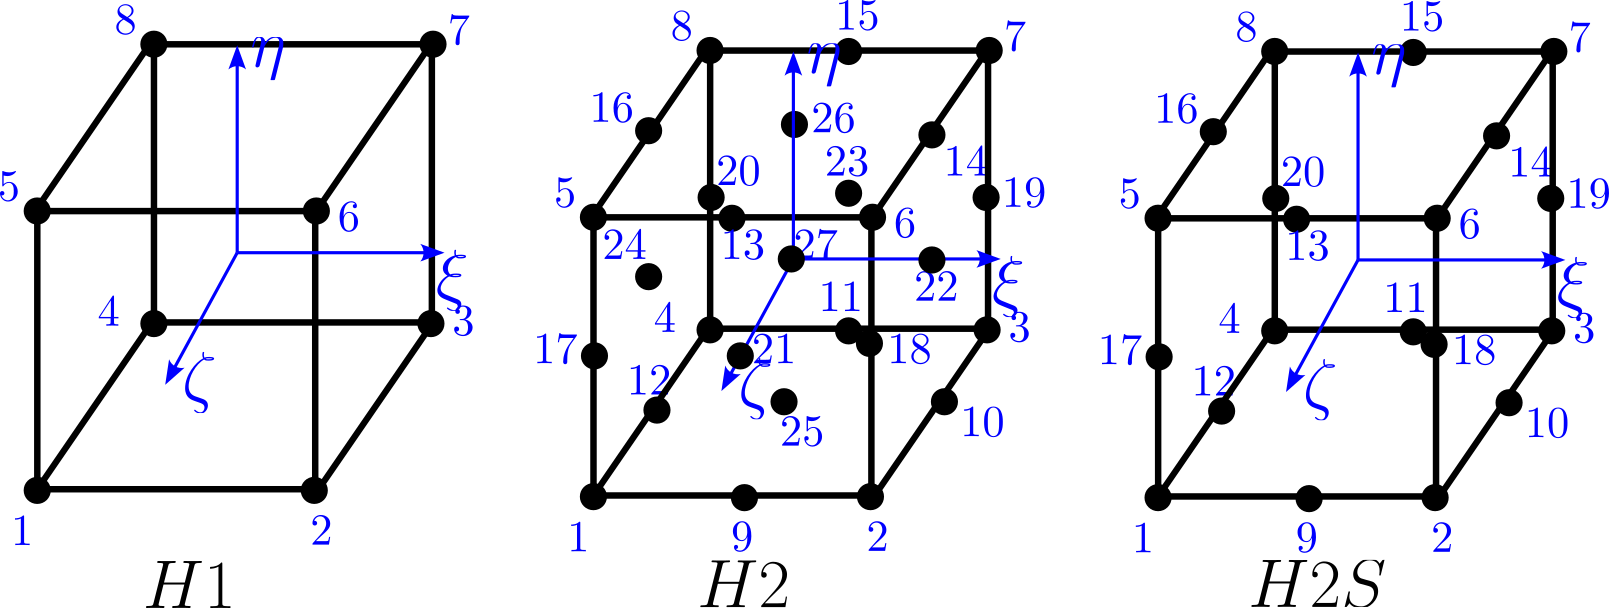
\includegraphics[width=0.625\linewidth]{files/HexElements-a4ee848a8b573d56dbd74d399701e925.png}
\caption[]{3D-Hexaeder-Elemente mit linearer (8 Knoten) und quadratischer (27 Knoten) Approximation. Zusätzlich ist das 20-Knoten-Hexaeder-Serendipity-Element gezeigt.}
\label{hexElements}
\end{figure}

Im 3D-Fall werden die Formfunktionen für Hexaeder-Elemente als Tensorprodukt der 1D-Formfunktionen definiert. Für ein 3D-Hexaeder-Element mit 8 Knoten (lineares Element) sind die Formfunktionen:

\begin{align}
N_1 &= \frac{1}{8} (1 - \xi)(1 - \eta)(1 - \zeta) & N_2 &= \frac{1}{8} (1 + \xi)(1 - \eta)(1 - \zeta) \\
N_3 &= \frac{1}{8} (1 + \xi)(1 + \eta)(1 - \zeta) & N_4 &= \frac{1}{8} (1 - \xi)(1 + \eta)(1 - \zeta) \\
N_5 &= \frac{1}{8} (1 - \xi)(1 - \eta)(1 + \zeta) & N_6 &= \frac{1}{8} (1 + \xi)(1 - \eta)(1 + \zeta) \\
N_7 &= \frac{1}{8} (1 + \xi)(1 + \eta)(1 + \zeta) & N_8 &= \frac{1}{8} (1 - \xi)(1 + \eta)(1 + \zeta)
\end{align}

Um ein vollständiges Element der Ordnung 2 zu erhalten, benötigt man 27 Knoten beim Hexaeder-Element. Die Formfunktionen kann man zum Beispiel \cite{wriggers2008nonlinear} entnehmen. Mehr Verwendung findet das 20-Knoten-Element. Hierbei handelt es sich um ein Serendipity-Element, das nicht vollständig von der Ordnung 2 ist, aber die Bedingungen der Raumisotropie, keine Verformung bei starren Körperbewegungen und die Möglichkeit, konstante Spannungszustände zu modellieren, erfüllt.

Für tetraedrische Elemente implementieren gängige FEM-Programme Tetraeder mit entweder 4 oder 10 Knoten. Diese sind in Abbildung Figure~\ref{tetraElements} dargestellt.

\begin{figure}[!htbp]
\centering
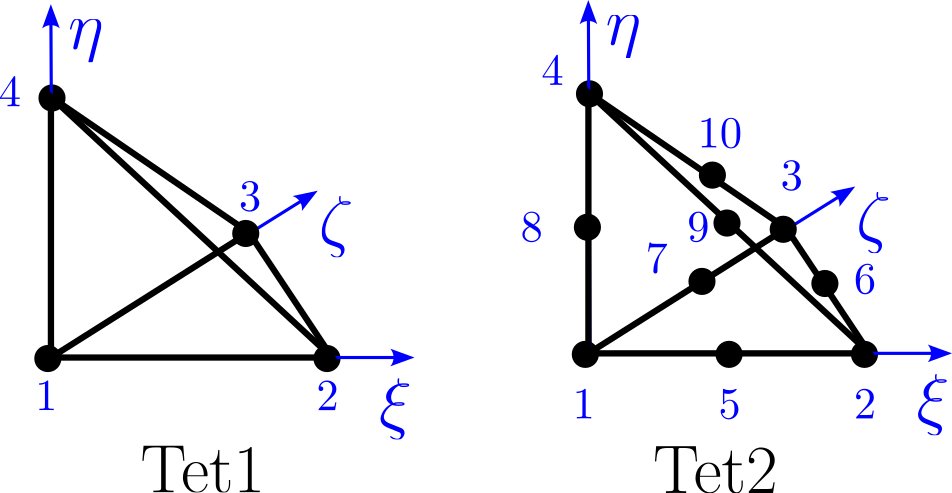
\includegraphics[width=0.625\linewidth]{files/TetElements-996ee625624fda771512d85c968c03fc.png}
\caption[]{Tetraedrische Elemente mit linearen (Tet1) und quadratischen (Tet2) Formfunktionen.}
\label{tetraElements}
\end{figure}

Die linearen Tetraederelemente (T4) sind die einfachsten und werden häufig als ``konstante'' Elemente in der Literatur bezeichnet, wobei sich dies auf die abgeleiteten Grö$\beta$en (z.B. Spannungen, Dehnungen, etc.) bezieht. Die Formfunktionen lauten:

\begin{align}
\lambda &= 1 - \xi - \eta - \zeta & N_1(\xi ,\eta ,\zeta ) &= \lambda \\
N_2(\xi ,\eta ,\zeta ) &= \xi & N_3(\xi ,\eta ,\zeta ) &= \eta & N_4(\xi ,\eta ,\zeta ) &= \zeta
\end{align}

Die Formfunktionen für tetraedrische Elemente mit 10 Knoten (T10) sind vollständig quadratisch und bieten bessere Approximationseigenschaften als das T4-Element. Die Formfunktionen lauten:

\begin{align}
\lambda &= 1 - \xi - \eta - \zeta & N_1(\xi ,\eta ,\zeta ) &= \lambda (2\lambda - 1) \\
N_2(\xi ,\eta ,\zeta ) &= \xi (2\xi - 1) & N_3(\xi ,\eta ,\zeta ) &= \eta (2\eta - 1) \\
N_4(\xi ,\eta ,\zeta ) &= \zeta (2\zeta - 1) & N_5(\xi ,\eta ,\zeta ) &= 4\lambda \xi \\
N_6(\xi ,\eta ,\zeta ) &= 4\xi \eta & N_7(\xi ,\eta ,\zeta ) &= 4\lambda \eta \\
N_8(\xi ,\eta ,\zeta ) &= 4\lambda \zeta & N_9(\xi ,\eta ,\zeta ) &= 4\xi \zeta \\
N_{10}(\xi ,\eta ,\zeta ) &= 4\eta \zeta
\end{align}

\begin{framed}
\textbf{Fragen zum Kapitel}\\
\textbf{Ansatzfunktionen}

\begin{itemize}
\item Wieviele Knoten hat ein Tetraeder-Element mit linearen Ansatzfunktionen?
\item Wieviele Knoten hat ein Viereck-Element mit quadratischen Ansatzfunktionen?
\item Eine wichtige Eigenschaft der gezeigten Formfunktionen ist, dass sie nur am zugehörigen Knoten den Wert 1 annehmen. An allen anderen Knoten ist der Wert 0. Was bedeutet dies für den Knotenfreiheitsgrad bzgl. seiner physikalischen Deutbarkeit?
\item Welche Aussage ist richtig?\begin{itemize}
\item Bei Formfunktionen mit quadratischem Polynomgrad ist der Verlauf der Dehnungen im Element quadratisch.
\item Bei Formfunktionen mit linearem Verlauf sind die Verschiebungen im Element linear.
\item Die Dehnungen sind über die Elementränder hinweg stetig für Formfunktionen mit quadratischem Polynomgrad.
\item Die Summe der Ansatzfunktionen im Element ist stets 1.
\end{itemize}
\end{itemize}
\end{framed}

\subsubsection{Integration}

Betrachten wir die schwache Form der Impulsbilanz:

\begin{equation}
\int_{\mathcal{B}} \delta\eb\T  \bm{\sigma} \dV = \int_{\mathcal{B}} \delta \bm{u}\T \rho \bm{b} \dV + \int_{\partial\mathcal{B}} \delta \bm{u}\T  \bm{t} \dA \; .
\end{equation}

Dass die Ableitung der Testfunktion $\delta \bm{u}$ und der Verschiebung $\bm{u}$ berechnet werden muss, wurde bereits im vergangenen Abschnitt erläutert. Zusätzlich muss der Term $\delta\eb\T  \bm{\sigma}$ über das gesamte Volumen des Körpers $\mathcal{B}$ integriert werden. Dabei wird in der Finite-Elemente-Methode die Integration über das Volumen des Körpers $\mathcal{B}$ in eine Summe über die Volumen der Elemente $\mathcal{B}^e$ zerlegt:

\begin{equation}
\int_{\mathcal{B}} \delta\eb\T  \bm{\sigma} \dV = \bigcup_{e=1}^{n_{\text{el}}} \int_{\mathcal{B}^e} \delta\eb\T  \bm{\sigma} \dV_e \; .
\end{equation}

Nun kann die Integration auf Elementebene durchgeführt werden. Diese sind aber in der Regel krummlinig berandet und die Integration über das Volumen eines Elements $\mathcal{B}^e$ ist nicht trivial. Daher wird die Integration über das Volumen des Elements $\mathcal{B}^e$ in eine Integration über das Volumen des Referenzelements $\mathcal{B}_{\square}$ umgewandelt:

\begin{equation}
\int_{\mathcal{B}^e} \delta\eb\T  \bm{\sigma} \dV_e = \int_{\mathcal{B}_{\square}} \delta\eb\T  \bm{\sigma} \left| \bm{J} \right| \dV_{\square} \; .
\end{equation}

Dabei ist $\left| \bm{J} \right|$ die Determinante der Jacobi-Matrix $\bm{J}$, die die Transformation von $\mathcal{B}_{\square}$ nach $\mathcal{B}^e$ beschreibt. Damit können wir die Funktion $\delta\eb\T  \bm{\sigma}$ jetzt über eine sehr einfache Geometrie integrieren. Sowohl der Integrand $\delta\eb\T  \bm{\sigma}$ als auch die Determinante der Jacobi-Matrix $\left| \bm{J} \right|$ sind in der Regel nicht konstant, ja sogar gebrochen rationale Funktionen. Die Integrale können daher nicht analytisch gelöst werden. Die bisherige exakte Transformation des Integrals muss nun durch eine numerische Integration approximiert werden. Die numerischen Integrationsformeln werden im Folgenden auch als \textit{Quadraturformeln} bezeichnet. Allgemein gilt für eine Quadraturformel:

\begin{equation}
\int_{\mathcal{B}_{\square}} f(\bm{\xi}) \dV_{\square} \approx \sum_{i=1}^{n_{\text{qp}}} w_i f(\bm{\xi}_i) \; .
\end{equation}

Die Integration der Funktion $f(\bm{\xi})$ über das Gebiet $\mathcal{B}_{\square}$ wird also ersetzt durch eine Summe über die Funktionswerte $f(\bm{\xi}_i)$ an den Integrationspunkten $\bm{\xi}_i$, multipliziert mit den Gewichten $w_i$. Die Anzahl der Integrationspunkte $n_{\text{qp}}$ hängt von der gewünschten Genauigkeit der Integration ab. Die Integrationspunkte und Gewichte sind für die im vorangegangenen Abschnitt beschriebenen Elemente in Tabellen zusammengestellt. Die Genauigkeit der Integration hängt ma$\beta$geblich von der Form der Funktion $f(\bm{\xi})$ ab. Allgemein gilt, dass die Genauigkeit der Integration mit der Anzahl der Integrationspunkte steigt. Die in den FE-Programmen meist verwendeten Integrationspunkte und Gewichte entsprechen den Gau$\beta$-Quadraturregeln oder sind zumindest an diese angelehnt. Bei der Gau$\beta$-Quadraturregel werden die Integrationspunkte so gewählt, dass die Integration einer Polynomfunktion $f(\bm{\xi})$ bis zu einem bestimmten Grad genau ist. Die Gewichte $w_i$ sind so gewählt, dass die Summe der Gewichte gleich der Fläche des Integrationsgebiets ist. Mit einer Integrationsordnung $m$ kann mit der Gau$\beta$-Quadratur ein Polynom $(2m - 1)$-ten Grades exakt integriert werden. Betrachten wir erneut die schwache Form und schreiben den Integranden $\delta\eb\T  \bm{\sigma}$ als $\delta\eb\T  \bm{\sigma} = \delta\eb\T  \mathbb{C} \eb$, dann sehen wir, dass rechts und links der Materialtangente $\mathbb{C}$ die räumliche Ableitung von $\bm{u}_h$ und $\delta\bm{u}_h$ steht. Wenn wir nun quadratische Formfunktionen verwenden, dann ist die Ableitung der Formfunktionen zumindest in einer Koordinatenrichtung weiterhin quadratisch. Durch die Multiplikation im Integranden müssen wir also ein Polynom 4. Grades integrieren. Nach der obigen Definition ist hierfür eine Quadraturformel 3. Grades erforderlich.

\begin{framed}
\textbf{Notwendige Ordnung der Integration}\\
Für die Integration der Steifigkeitsmatrix der FEM mit Elementen mit Formfunktionen der Ordnung $n$ ist eine Quadraturformel der Ordnung:

\begin{equation*}
m = \frac{n+1}{2}
\end{equation*}
erforderlich.
\end{framed}

Nachfolgende Tabellen zeigen die 1D- und 2D-Quadraturformeln.

\begin{figure}[!htbp]
\centering
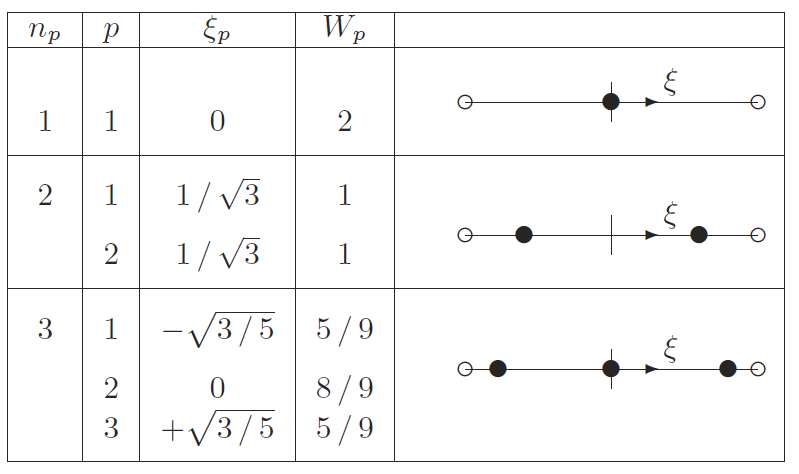
\includegraphics[width=0.625\linewidth]{files/Wriggers_GQ_01-1fe6a7f6344b6ab2a225d181d5bca432.png}
\caption[]{1D-Gau$\beta$-Quadraturformeln für verschiedene Ordnungen $m$ nach \cite{wriggers2008nonlinear}.}
\label{lineQuadrature}
\end{figure}

\begin{figure}[!htbp]
\centering
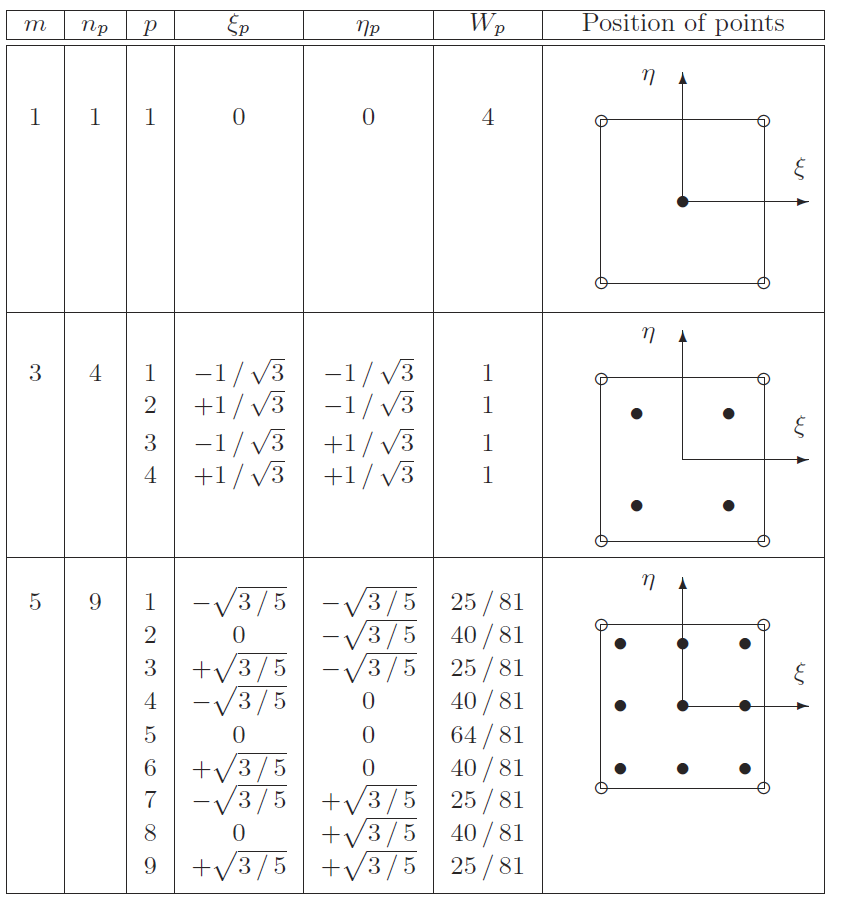
\includegraphics[width=0.625\linewidth]{files/Wriggers_GQ_02-d7a6daa03fb1eafb11f2f6a808c915f2.png}
\caption[]{2D-Gau$\beta$-Quadraturformeln für Rechteckelemente verschiedener Ordnung $m$ nach \cite{wriggers2008nonlinear}.}
\label{squareQuadrature}
\end{figure}

\begin{figure}[!htbp]
\centering
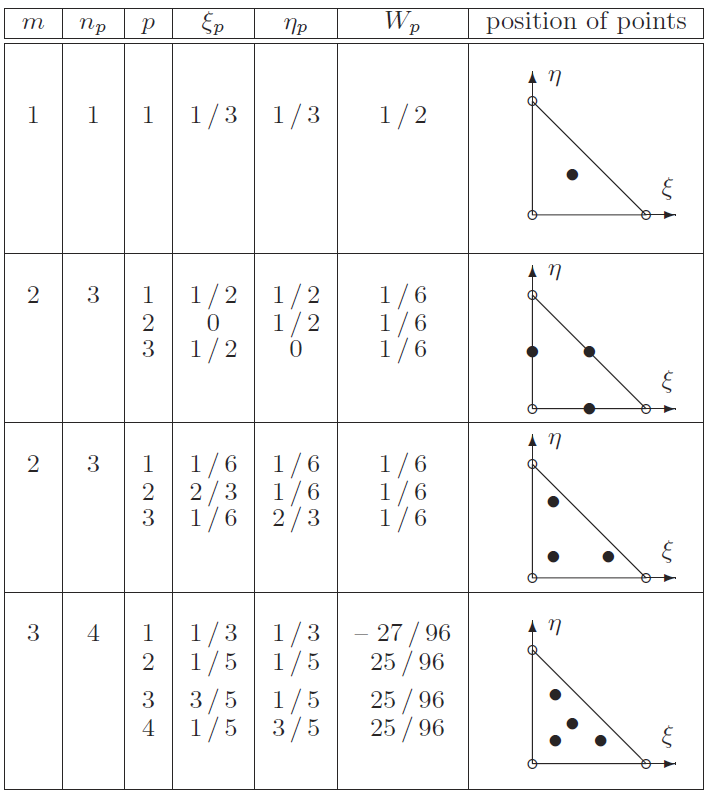
\includegraphics[width=0.625\linewidth]{files/Wriggers_GQ_03-44827e8d787266f893a14150a814a302.png}
\caption[]{2D-Gau$\beta$-Quadraturformeln für Dreieckselemente verschiedener Ordnung $m$ nach \cite{wriggers2008nonlinear}.}
\label{triQuadrature}
\end{figure}

\paragraph{Beispiel: 1D-Integration}

Wir möchten das Polynom $f(x) = \frac{1}{2} x^4 + 6x + 4$ über das Intervall $[ -1,1]$ integrieren. Die exakte Lösung ist:
\begin{equation*}
\int_{-1}^{1} \left(\frac{1}{2} x^4 + 6x + 4\right) \, \mathrm{d}x = \left[\frac{1}{10} x^5+2x^3+4x \right]_{-1}^{1} = 12.2
\end{equation*}

Da wir im Intervall $[ -1,1]$ integrieren, können wir direkt die Gau$\beta$-Quadraturformeln verwenden. Wir müssen nicht die Jacobideterminante berechnen.
Verwenden wir jetzt eine Integrationsordnung mit einem Integrationspunkt, so ergibt sich:
\begin{align*}
\xi_p &= 0  & w_p &= 2 \\
\int_{-1}^{1} f(x) \, \mathrm{d}x &= \sum_{p=1}^{1} w_p f(\xi_p) \\
\int_{-1}^{1} f(x) \, \mathrm{d}x &= 2 \cdot 4  = 8
\end{align*}

Mit dieser Integrationsordnung ergibt sich also ein Fehler von 34 \%.

Als nächstes nehmen wir eine Integrationsordnung mit zwei Integrationspunkten:
\begin{align*}
\xi_p &= \pm \frac{1}{\sqrt{3}} & w_p &= 1 \\
\int_{-1}^{1} f(x) \, \mathrm{d}x &= \sum_{p=1}^{2} w_p f(\xi_p)  \\
\int_{-1}^{1} f(x) \, \mathrm{d}x &= 1 \cdot 6.06  + 1 \cdot 6.06 = 12.111
\end{align*}

Hier ergibt sich nur noch ein Fehler von 1 \%.

Erst eine Integrationsordnung mit drei Integrationspunkten liefert das exakte Ergebnis:
\begin{align*}
\xi_p &= 0, \pm \sqrt{\frac{3}{5}} & w_p &= \frac{8}{9}, \frac{5}{9} \\
\int_{-1}^{1} f(x) \, \mathrm{d}x &= \sum_{p=1}^{3} w_p f(\xi_p) \\
\int_{-1}^{1} f(x) \, \mathrm{d}x &= \frac{5}{9} \cdot 7.78  + \frac{8}{9} \cdot 4 + \frac{5}{9} \cdot 7.78  = 12.2
\end{align*}

\begin{framed}
\textbf{Fragen zum Kapitel}\\
\textbf{Integration}

\begin{itemize}
\item Warum müssen wir die schwache Form der Impulsbilanz numerisch integrieren?
\item Wie lautet die allgemeine Formel für die Quadratur einer Funktion $f(x)$ über ein Referenzgebiet?
\item Wie lässt sich die Genauigkeit der numerischen Integration erhöhen?
\item Welche Aussage ist richtig?\begin{itemize}
\item Eine Erhöhung der Integrationsordnung führt zu einer höheren Genauigkeit.
\item Eine Erhöhung der Integrationsordnung führt zu einer höheren Anzahl an Integrationspunkten.
\item Bei zu wenigen Integrationspunkten verhält sich das Element zu ``weich''.
\item Unzulässige Null-Energiemodi sind ein Indikator für zu wenige Integrationspunkte.
\item Ist die notwendige Anzahl an Integrationspunkten erreicht, führt auch eine Erhöhung der Integrationsordnung nicht zu einer besseren Konvergenz.
\end{itemize}
\end{itemize}
\end{framed}

\subsubsection{Postprocessing}

Das Postprocessing stellt einen unverzichtbaren Schritt in der Finite-Elemente-Analyse (FEA) dar. Es ist definiert als der Prozess der Transformation und Aufbereitung der oft hochdetaillierten und komplexen Rohausgaben von FEM-Berechnungen in ein für den Anwender leicht verständliches Format. Im Wesentlichen handelt es sich um die Modifikation oder Verbesserung von Ergebnisdaten, nachdem eine Lösung aus einem Rechenmodell erhalten wurde, mit dem Ziel, aussagekräftige Visualisierungen, Diagramme und andere Ausgaben zu erstellen.

\begin{figure}[!htbp]
\centering
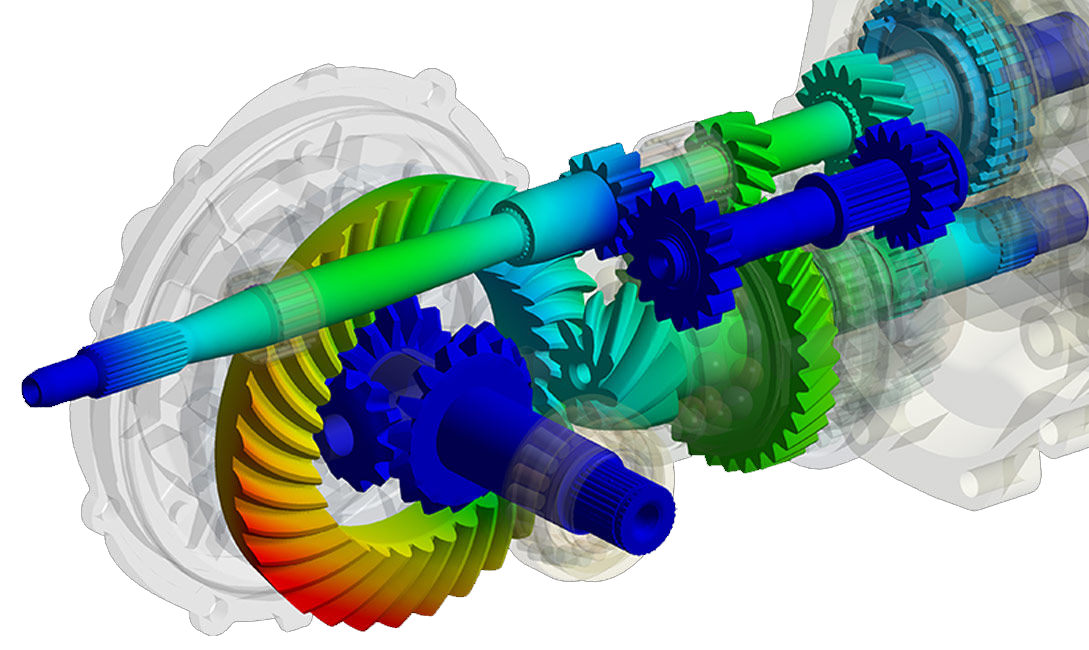
\includegraphics[width=0.625\linewidth]{files/postproc_ansys-7b8042d4d341e019c0ffa102e0eee386.png}
\caption[]{Postprocessing in ANSYS Mechanical nach \href{https://www.padtinc.com/simulation/simulation-product/ansys-mechanical/}{link}.}
\label{postprocansys}
\end{figure}

\paragraph{Postprocessing primärer Grö$\beta$en}

In der Finite-Elemente-Analyse werden die sogenannten primären Grö$\beta$en direkt als Ergebnis der Lösung des globalen Gleichungssystems berechnet. Typische Beispiele hierfür sind Verschiebungen in der Strukturmechanik oder Temperaturen in der Wärmeübertragung. Diese Grö$\beta$en werden explizit an den Knoten des Finite-Elemente-Netzes ermittelt. Die resultierenden Knotenverschiebungen gelten als präzise, da jedem Knoten innerhalb des Netzes ein einziger, eindeutiger Verschiebungswert zugewiesen wird. Dies unterscheidet sich grundlegend von den sekundären Grö$\beta$en, die später erläutert werden.\newline
Die Werte der primären Feldvariablen, die an den diskreten Knoten berechnet werden, dienen dazu, die Werte an allen anderen Punkten innerhalb eines Elements  zu approximieren. Dies geschieht durch Interpolation der Knotenwerte mittels der Formfunktionen des Elementes.
Dies gewährleistet die Inter-Element-Kontinuität der primären Feldvariablen (z.B. Verschiebung oder Temperatur) an den Knotenpunkten. Die Formfunktionen stellen somit die mathematische Brücke dar, die es ermöglicht, die diskrete Lösung an den Knoten in ein kontinuierliches Feld innerhalb jedes Elements zu überführen. Diese Interpolationsfähigkeit ist von grundlegender Bedeutung für die FEM, da sie es erlaubt, mit einer endlichen Anzahl von Freiheitsgraden ein kontinuierliches physikalisches Phänomen anzunähern.

\bigskip\noindent
\begin{tabular}{p{\dimexpr 0.333\linewidth-2\tabcolsep}p{\dimexpr 0.333\linewidth-2\tabcolsep}p{\dimexpr 0.333\linewidth-2\tabcolsep}}
\toprule
Kriterium & Primäre Grö$\beta$en (z.B. Verschiebung, Temperatur) & Sekundäre Grö$\beta$en (z.B. Spannung, Dehnung, Moment) \\
\hline
\textbf{Typ} & Feldvariablen, direkte Lösung & Abgeleitete Grö$\beta$en \\
\textbf{Berechnungspunkt} & Knoten & Gau$\beta$punkte (dann zu Knoten extrapoliert) \\
\textbf{Kontinuität} & C0-kontinuierlich (an Knoten) & Diskontinuierlich an Elementgrenzen \\
\textbf{Genauigkeit (relativ)} & Präzise (eindeutiger Wert pro Knoten) & Weniger präzise (aber genauer an Gau$\beta$punkten) \\
\textbf{Rolle im Postprocessing} & Direkte Ausgabe, Visualisierung & Erfordert Glättung für physikalische Interpretation \\
\bottomrule
\end{tabular}

\bigskip\paragraph{Postprocessing sekundärer Grö$\beta$en}

\begin{figure}[!htbp]
\centering
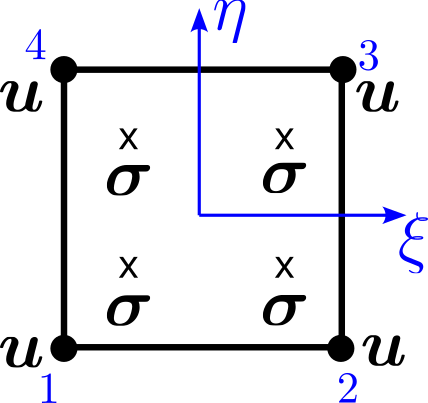
\includegraphics[width=0.375\linewidth]{files/FEM_Postprocessing-c22cc0dbfe91e308fcde8dfd97d168c0.png}
\caption[]{Unterschied zwischen primären und sekundären Grö$\beta$en im Postprocessing.}
\label{postprocFEM}
\end{figure}

Im Gegensatz zu primären Grö$\beta$en werden sekundäre Grö$\beta$en, wie Spannungen, Dehnungen und Momente, nicht direkt an den Knoten berechnet. Stattdessen werden diese abgeleiteten Grö$\beta$en an den sogenannten Gau$\beta$-Integrationspunkten innerhalb jedes Finite-Elements ermittelt.\newline
Der Grund für die Berechnung an Gau$\beta$punkten liegt in der mathematischen Formulierung der FEM, insbesondere im Rahmen der Galerkin-Methode. Die Berechnung von Spannungen und Dehnungen erfolgt aus den Ableitungen der Verschiebungsfelder. Die Gau$\beta$punkte sind die optimalen Punkte für die numerische Integration der Steifigkeitsmatrizen und Lastvektoren und bieten die genauesten Stellen zur Bestimmung dieser abgeleiteten Grö$\beta$en. Der Element-Solver ``kennt'' die Dehnung innerhalb des Elements basierend auf den Knotenverschiebungen und kann daraus die Spannung berechnen. Es ist jedoch wichtig zu verstehen, dass das Element kein ``vollständiges Wissen'' über das Geschehen in seinem Inneren besitzt; es prognostiziert lediglich einige korrekte Antworten an den Gau$\beta$punkten und schätzt bzw. extrapoliert diese wenigen genauen Antworten auf den Rest seiner Fläche.\newline
Um die an den Gau$\beta$punkten berechneten Werte der sekundären Grö$\beta$en an den Knotenpositionen zu erhalten, ist eine Extrapolation dieser Werte von den Gau$\beta$punkten zu den Knoten erforderlich. Diese Extrapolation ist notwendig, da die Knoten oft die primären Punkte für die Ergebnisdarstellung und -interpretation sind.\newline
Es existieren verschiedene Methoden zur Extrapolation von Gau$\beta$punktwerten zu den Knoten, die jeweils unterschiedliche Implikationen für die Ergebnisdarstellung und -genauigkeit haben:

\begin{itemize}
\item \textbf{Zentroidaler Wert (Centroidal Value):} Bei dieser einfachen Methode wird der Durchschnitt der Gau$\beta$punkt-Ergebnisse über alle Gau$\beta$punkte eines Elements berechnet und dieser gemittelte Wert allen Knoten des jeweiligen Elements zugewiesen. Dies führt zu einer sehr starken Glättung der Ergebnisse innerhalb eines Elements.


\item \textbf{Nodalwerte, extrapoliert von Gau$\beta$punkten (Nodal Values Extrapolated from Gauss Points):} Diese Methode verwendet lineare Formfunktionen, um die Gau$\beta$punktwerte zu den Knoten zu extrapolieren. Die Extrapolation entspricht einem Least-Squares-Fit. Sie wird im Allgemeinen für die Mehrheit der linearen Materialmodelle bevorzugt. Eine wichtige Einschränkung ist jedoch, dass diese Option für nichtlineare Materialien unter Umständen nicht gültig ist, da die Extrapolation von Gau$\beta$punktspannungen zu den Knoten zu nodalen Spannungen führen könnte, die die Materialgrenzen überschreiten, was physikalisch inkorrekt wäre.


\item \textbf{Gau$\beta$punktwerte direkt an Knoten platziert (Gauss Point Values Placed at Nodes):} Hierbei wird jedes Gau$\beta$punkt-Ergebnis direkt seinem nächstgelegenen Knoten zugewiesen, ohne weitere Extrapolation. Diese Option ist in der Regel am zuverlässigsten für nichtlineare Materialien, da die direkt zugewiesenen Knotenwerte niemals die Materialgrenzen überschreiten werden.
\end{itemize}

Die grundlegende Natur sekundärer Grö$\beta$en als ``abgeleitete'' Grö$\beta$en hat weitreichende Auswirkungen auf ihre Genauigkeit. Während primäre Grö$\beta$en direkt aus der Lösung der Gleichgewichtsgleichungen resultieren, werden sekundäre Grö$\beta$en durch Rücksubstitution aus den primären Grö$\beta$en berechnet. Da die FEM eine Näherungstechnik ist, propagieren Fehler in den primären Grö$\beta$en und können sich in den abgeleiteten sekundären Grö$\beta$en sogar verstärken, was zu einer höheren Fehleranfälligkeit führt (siehe Konvergenzanalyse der Querkraft bei der Balken-FEM). Die Wahl der Extrapolationsmethode ist somit nicht willkürlich, sondern hängt ma$\beta$geblich vom Materialmodell ab. Eine lineare Extrapolation kann für nichtlineare Materialien physikalisch unmögliche Ergebnisse liefern, was eine konservativere, direkte Zuweisung erforderlich macht. Dies verdeutlicht die Notwendigkeit, das zugrunde liegende Materialverhalten und dessen Wechselwirkung mit den numerischen Methoden genau zu verstehen, da dies die Gültigkeit und den physikalischen Realismus der postprozessierten Ergebnisse direkt beeinflusst.

\bigskip\noindent
\begin{tabular}{p{\dimexpr 0.250\linewidth-2\tabcolsep}p{\dimexpr 0.250\linewidth-2\tabcolsep}p{\dimexpr 0.250\linewidth-2\tabcolsep}p{\dimexpr 0.250\linewidth-2\tabcolsep}}
\toprule
Methode & Prinzip & Anwendungsbereich / Vorteile & Nachteile / Überlegungen \\
\hline
\textbf{Zentroidaler Wert} & Durchschnitt aller Gau$\beta$punktwerte eines Elements wird allen Knoten zugewiesen. & Einfache, schnelle Glättung. & Stark geglättet, verliert lokale Details. \\
\textbf{Nodalwerte, extrapoliert von Gau$\beta$punkten} & Lineare Formfunktionen extrapolieren Gau$\beta$punktwerte zu Knoten. & Bevorzugt für lineare Materialmodelle. & Kann bei nichtlinearen Materialien Materialgrenzen überschreiten. \\
\textbf{Gau$\beta$punktwerte direkt an Knoten platziert} & Jedes Gau$\beta$punkt-Ergebnis wird direkt dem nächstgelegenen Knoten zugewiesen. & Am zuverlässigsten für nichtlineare Materialien, da Materialgrenzen nicht überschritten werden. & Führt zu Diskontinuitäten an Elementgrenzen, da keine Glättung erfolgt. \\
\bottomrule
\end{tabular}

\bigskip\begin{framed}
\textbf{Fragen zum Kapitel}\\
\textbf{Postprocessing}

\begin{itemize}
\item Was sind primäre Grö$\beta$en der FEM in der Strukturmechanik und in der Wärmeleitung?
\item Wo liegen die primären Grö$\beta$en vor?
\item Wo liegen die sekundären Grö$\beta$en bei der FEM vor?
\item Warum werden sekundäre Grö$\beta$en an Gau$\beta$-Integrationspunkten berechnet und nicht direkt an den Knoten?
\item Welche Methoden existieren, um sekundäre Grö$\beta$en von Gau$\beta$punkten zu den Knoten zu extrapolieren?
\item Was ist ein Indikator für eine konvergierte Lösung einer sekundären Grö$\beta$e?
\end{itemize}
\end{framed}

\section{Praktisches zur Anwendung der FEM}

\subsection{Praktische Hinweise zur Anwendung der FEM}

In den nachfolgenden Abschnitten sind Themen der Praktika zusammengefasst. Dieser Abschnitt ist noch im Aufbau und unvollständig.

\input{FEMI_Skript-symmetrie}

\input{FEMI_Skript-fehlerquellen}

\input{FEMI_Skript-vernetzung}

\chapter{Modul: Spezielle Gebiete der FEM}

\input{FEMI_Skript-modalanalyse}

\chapter{Quellenverzeichnis}


\input{FEMI_Skript-quellen}




\bibliography{main.bib}

\end{document}
